% =====================================================================
%  Breaking ECDSA on a fault-tolerant quantum computer
%  The ECDSA.fail optimisations, the Pareto frontier, and the cost of
%  error correction --- written for the shor/ project
%  Build:  pdflatex main && bibtex main && pdflatex main && pdflatex main
%  (or:    latexmk -pdf main)
% =====================================================================
\documentclass[11pt,a4paper]{article}
\usepackage[margin=2.3cm]{geometry}
\usepackage[T1]{fontenc}
\usepackage[utf8]{inputenc}
\usepackage{mathpazo}          % Palatino (URW Type 1, scalable) for text and maths
\usepackage[scaled=0.92]{helvet}
\usepackage{courier}
\usepackage[expansion=false]{microtype}
\usepackage{amsmath,amssymb,amsthm,mathtools}
\usepackage{booktabs,multirow,array,longtable}
\usepackage{xcolor}
\usepackage{graphicx}
\usepackage{enumitem}
\usepackage{siunitx}
\usepackage{tikz}
\usetikzlibrary{arrows.meta,calc,positioning,decorations.pathreplacing,fit,shapes.geometric,backgrounds,patterns,matrix,quantikz2}
\usepackage{pgfplots}
\pgfplotsset{compat=1.18}
\pgfplotsset{discard if not/.style 2 args={x filter/.append code={\edef\tempa{\thisrow{#1}}\edef\tempb{#2}\ifx\tempa\tempb\else\def\pgfmathresult{inf}\fi}}}
\usepackage{pgfplotstable}
\usepackage{caption,subcaption}
\usepackage{float}
\usepackage{placeins}
\usepackage{algorithm}
\usepackage[noend]{algpseudocode}
\usepackage{listings}
\usepackage[most]{tcolorbox}
\usepackage[numbers,sort&compress]{natbib}
\usepackage{xurl}
\usepackage[colorlinks,linkcolor=blue!55!black,citecolor=blue!55!black,urlcolor=blue!55!black]{hyperref}
\usepackage[capitalise,noabbrev]{cleveref}

% ---------------------------------------------------------------- macros
\renewcommand{\ket}[1]{\lvert #1 \rangle}
\renewcommand{\bra}[1]{\langle #1 \rvert}
\providecommand{\braket}[2]{\langle #1 \vert #2 \rangle}
\newcommand{\F}{\mathbb{F}}
\newcommand{\Z}{\mathbb{Z}}
\newcommand{\C}{\mathbb{C}}
\newcommand{\id}{\mathbb{1}}
\newcommand{\Tof}{\mathrm{Tof}}
\newcommand{\code}[1]{\texttt{#1}}
\emergencystretch=2.5em
\newcommand{\ecdsafail}{ECDSA.fail}
\newcommand{\QT}{Q\times T}
\newcommand{\dd}{\mathrm{d}}
\newcommand{\MAJ}{\mathrm{MAJ}}
\newcommand{\UMA}{\mathrm{UMA}}
\newcommand{\Hmr}{\mathrm{Hmr}}
\newcommand{\bits}[3]{[\![#1,#2,#3]\!]}
\DeclareMathOperator{\wt}{wt}
\DeclareMathOperator{\rank}{rank}
\DeclareMathOperator{\bitlen}{bitlen}
\DeclareMathOperator{\rot}{rot}
\DeclareMathOperator{\gcdop}{gcd}

\theoremstyle{plain}
\newtheorem{theorem}{Theorem}[section]
\newtheorem{lemma}[theorem]{Lemma}
\newtheorem{proposition}[theorem]{Proposition}
\newtheorem{corollary}[theorem]{Corollary}
\theoremstyle{definition}
\newtheorem{definition}[theorem]{Definition}
\newtheorem{example}[theorem]{Example}
\theoremstyle{remark}
\newtheorem*{remark}{Remark}

\definecolor{boxblue}{RGB}{22,63,110}
\definecolor{boxred}{RGB}{140,38,28}
\definecolor{boxgreen}{RGB}{30,95,60}
\definecolor{gateblue}{RGB}{242,246,251}
\definecolor{lookorange}{RGB}{255,245,231}
\definecolor{addviolet}{RGB}{244,242,251}
\definecolor{outgreen}{RGB}{239,248,242}
\definecolor{cX}{RGB}{214,96,77}
\definecolor{cZ}{RGB}{67,147,195}
\definecolor{cY}{RGB}{120,120,120}
\definecolor{cdata}{RGB}{40,40,40}
\newtcolorbox{keybox}[1][]{colback=boxblue!4,colframe=boxblue,coltitle=white,
  fonttitle=\bfseries,boxrule=0.7pt,left=6pt,right=6pt,top=5pt,bottom=5pt,#1}
\newtcolorbox{warnbox}[1][]{colback=boxred!4,colframe=boxred,coltitle=white,
  fonttitle=\bfseries,boxrule=0.7pt,left=6pt,right=6pt,top=5pt,bottom=5pt,#1}
\newtcolorbox{srcbox}[1][]{colback=boxgreen!4,colframe=boxgreen,coltitle=white,
  fonttitle=\bfseries,boxrule=0.7pt,left=6pt,right=6pt,top=5pt,bottom=5pt,#1}

\definecolor{codebg}{RGB}{248,248,251}
\lstdefinestyle{py}{language=Python,basicstyle=\small\ttfamily,keywordstyle=\color{blue!60!black}\bfseries,
  commentstyle=\color{green!40!black}\itshape,stringstyle=\color{red!60!black},showstringspaces=false,
  backgroundcolor=\color{codebg},frame=single,framerule=0.3pt,rulecolor=\color{black!25},
  columns=fullflexible,keepspaces=true,breaklines=true,tabsize=4,aboveskip=6pt,belowskip=4pt}
\lstdefinestyle{plain}{basicstyle=\small\ttfamily,backgroundcolor=\color{codebg},frame=single,
  framerule=0.3pt,rulecolor=\color{black!25},columns=fullflexible,keepspaces=true,breaklines=true,aboveskip=6pt,belowskip=4pt}
\lstset{style=py}

\tikzset{
  wire/.style={black,line width=0.8pt},
  flow/.style={-{Latex[length=2mm,width=1.3mm]},line width=0.7pt},
  blk/.style={draw=black!70,line width=0.7pt,fill=gateblue,rounded corners=1.5pt,inner sep=4pt,align=center,font=\small},
  blkv/.style={blk,fill=addviolet},
  blko/.style={blk,fill=lookorange},
  blkg/.style={blk,fill=outgreen},
  stage/.style={draw=black!70,line width=0.7pt,fill=gateblue,rounded corners=1.5pt,inner sep=4pt,align=center,font=\footnotesize,text width=28mm,minimum height=22mm},
  note/.style={font=\footnotesize,text=black!70,align=center},
  dq/.style={circle,draw=cdata,fill=white,inner sep=0pt,minimum size=5pt},
  xface/.style={fill=cX!35,draw=black!60,line width=0.4pt},
  zface/.style={fill=cZ!35,draw=black!60,line width=0.4pt},
}

\sisetup{group-separator={,},group-minimum-digits=4}

\title{\bfseries Breaking ECDSA on a fault-tolerant quantum computer\\[4pt]
\large The \ecdsafail{} optimisations, the Pareto frontier, and the cost of quantum error correction}
\author{A companion to the \texttt{shor/} project\\[4pt]
\parbox{0.85\textwidth}{\centering\small Sources: arXiv, IACR ePrint, GitHub (the \ecdsafail{} challenge and its supplemental materials), and the published material of Google Quantum AI, IBM Quantum, IonQ, Quantinuum, PsiQuantum, QuEra and Alice\,\&\,Bob.}}
\date{12 October 2026}

\begin{document}
\maketitle
\vspace{-1.5em}

\begin{abstract}
\noindent
Shor's algorithm breaks the elliptic-curve digital signature algorithm by computing a discrete logarithm on secp256k1, and the cost of doing so is dominated by one reversible circuit: the in-place addition of a classically known point to a quantum accumulator. The \ecdsafail{} open-autoresearch challenge (May--October 2026) cut the width\,$\times$\,work product of that circuit from $2{,}715\times 3{,}960{,}753$ to $1{,}151\times 1{,}299{,}453$ by the paper's data cutoff and to $1{,}244\times 797{,}905$ on the 7~October leaderboard, while a separate low-width track reached $792$ logical qubits. Part~I of this document explains every optimisation family that produced that movement---the six inversion architectures (Kaliski, dialog GCD, Jump-2 with the base-5 codec, ping-pong, Skywalk, Leapfrog), the arithmetic levers (temporary-AND adders, chunked adders with measured carry erasure, truncated comparators, pseudo-Mersenne folds, Karatsuba squaring), the qubit levers (peak owners, budgets, venting, wire loans, register-shared Euclid, ghosting), measurement-based uncomputation, the post-passes, and the nonce-hunting economics that make approximate circuits pass a finite validator---with the circuit diagrams of the supplemental notes redrawn, and it gives the Pareto frontier in both the challenge's $(Q,T)$ plane and the leaderboard's time axis, placed next to the external operating points of Google, Schrottenloher, TrailMix, Luo et al.\ and IonQ, and next to the circuits built in \texttt{shor/}. Part~II is about what it costs to run such a circuit on noisy hardware: the threshold theorem and the overhead of error correction, the stabiliser formalism with encoding and decoding algorithms spelled out in full for the small codes, the surface and toric codes (lattice, syndrome extraction, matching, union-find and neural decoders, lattice surgery), colour codes, and quantum LDPC codes (hypergraph products, bivariate bicycle codes such as IBM's gross code, belief propagation with ordered-statistics post-processing, IBM's bicycle architecture and IonQ's walking-cat architecture), the bounds of coding theory with the codes placed on the rate--distance plane, fault-tolerant Clifford gates (transversality, Eastin--Knill, lattice surgery, automorphisms, Pauli frames), fault-tolerant $T$ gates (magic-state injection, distillation, cultivation, code switching), and finally the physical-qubit estimates for a Clifford$+T$ computation, worked out for the \ecdsafail{} circuits and compared with the published superconducting, trapped-ion, neutral-atom and cat-qubit estimates. Every encoding circuit and the surface-code threshold plot were checked by simulation (Stim and PyMatching); the scripts are in the appendix.
\end{abstract}

\begin{keybox}[title={How to read this document}]
\textbf{Part I} (\cref{sec:target}--\cref{sec:shor-impl}) is about the \emph{logical} circuit: what \ecdsafail{} optimised, how each optimisation works, what it costs in the $\QT$ metric, and where the frontier stands. \textbf{Part II} (\cref{sec:qec-why}--\cref{sec:physical}) is about turning a logical circuit into a physical machine: codes, decoders, fault-tolerant gates, and the resulting physical-qubit and runtime estimates.

Notation. $p=2^{256}-2^{32}-977$ is the secp256k1 field prime, $r$ the (prime) group order, $n=256$. $Q$ is the peak number of live logical qubits of a circuit and $T$ its average number of \emph{executed} Toffoli gates (CCX/CCZ/AND) on the challenge's validation distribution; the challenge score is $S=\QT$. A $\bits{n}{k}{d}$ code uses $n$ physical qubits to encode $k$ logical qubits with distance $d$; $p$ also denotes a physical error rate where no confusion is possible, and $p_L$ a logical error rate. Numbers taken from a source are cited at the point of use; numbers computed for this document are marked as such and come from the scripts in \cref{app:scripts}.
\end{keybox}

{\small\setlength{\parskip}{0pt}\tableofcontents}
\clearpage

\part{The logical circuit: \ecdsafail{}}
\section{The target: ECDSA, secp256k1, and one reversible point addition}\label{sec:target}

\subsection{What a quantum computer has to compute}

ECDSA on secp256k1 signs with a secret scalar $k\in[1,r)$ whose public key is $Q=[k]P$, where $P$ is the standard generator of the curve
\[
E:\ y^2=x^3+7 \quad\text{over } \F_p,\qquad p=2^{256}-2^{32}-977,\qquad r=\#E(\F_p)\ \text{prime}.
\]
Verifying a signature needs only $Q$; forging one needs $k$; and recovering $k$ from $(P,Q)$ is the elliptic-curve discrete logarithm problem (ECDLP). Classically the best attacks are generic $\Theta(\sqrt r)\approx2^{128}$ group operations. Shor's algorithm \cite{shor97,proos-zalka03} solves it in polynomial time by phase estimation on the two-dimensional ``probe'' function
\begin{equation}\label{eq:probe}
f(u,v)=[u]P+[v]Q=[u+kv]P,\qquad f(u-k,\,v+1)=f(u,v),
\end{equation}
whose period lattice is generated by $(-k,1)$ and $(r,0)$: prepare two uniform superpositions over $u,v\in[0,2^m)$ with $2^m\gtrsim r$, compute $f$ coherently into a point register, Fourier-transform both scalar registers, and measure a pair $(s,t)$ that satisfies $t\equiv ks\pmod r$ with constant probability, from which $k=ts^{-1}\bmod r$ and the candidate is verified classically by $[k]P\overset{?}{=}Q$ \cite{ekera19}.

\begin{figure}[H]
\centering
\resizebox{\textwidth}{!}{%
\begin{quantikz}[column sep=6pt,row sep=5pt,font=\small]
\lstick{$\ket{u_0}$} & \qwbundle{16} & \gate{H^{\otimes16}} & \gate{\mathrm{lookup}} & \ctrl{6} & \gate{\mathrm{unlookup}} &          &         &          & \gate[3]{\mathcal F^{-1}} & \meter{} \\
\lstick{$\vdots$}     &  &                      &  &  &  & \ \cdots\ &         &          &                           &          \\
\lstick{$\ket{u_{15}}$} & \qwbundle{16} & \gate{H^{\otimes16}} &  &  &  &          & \ctrl{4}&          &                           & \meter{} \\
\lstick{$\ket{v_0}$} & \qwbundle{16} & \gate{H^{\otimes16}} &  &  &  &          &         & \ctrl{3} & \gate[3]{\mathcal F^{-1}} & \meter{} \\
\lstick{$\vdots$}     &  &                      &  &  &  &          &         &          &                           &          \\
\lstick{$\ket{v_{15}}$} & \qwbundle{16} & \gate{H^{\otimes16}} &  &  &  &          &         &          &                           & \meter{} \\
\lstick{$R:\ \ket{S}$} & \qwbundle{2\times256} &                   &  & \gate{+\,T_0[u_0]} & & \ \cdots\ & \gate{+\,T_{15}[u_{15}]} & \gate{+\,T'_{0}[v_0]} & \ \cdots &
\end{quantikz}}
\caption{Shor's ECDLP circuit with the scalars split into $16$-bit windows ($n=256$, $w=16$): each window $z\in\{u_j,v_j\}$ is a coherent address into a classical table $T_j[i]=[i\,2^{16j}]P$ (or $[i\,2^{16j}]Q$); a QROM lookup materialises the selected point, the accumulator $R$ is updated in place by one \emph{mixed} point addition, and the lookup is uncomputed. The scalar registers pass through unchanged and are read out by (semiclassical) inverse Fourier transforms. The accumulator starts at a fixed point $S$, never at $\mathcal O$, so that the affine formulas stay valid \cite{schrottenloher26,haener26}. Redrawn after Supplemental Note~D of \cite{ecdsafail26}.}
\label{fig:shor-ecdlp}
\end{figure}

\paragraph{Windowing and the cost formula.}
With $w$-bit windows there are $\lceil n/w\rceil=16$ windows per scalar, i.e.\ $32$ conceptual point additions; the first window is replaced by a direct table lookup of the $2^{2w}$ possible starting points (or $2^{18}$ entries in IonQ's version \cite{haener26}) and the last three windows are dropped and recovered by a classical search over $2^{48}$ candidates, which leaves $2n/w-4=28$ executed point additions \cite{babbush26,haener26,ecdsafail26}. Each addition also pays three table lookups of $2^{16}$ entries (the coordinates $x_A,y_A$ and the derived value $3x_A$), which both IonQ and \ecdsafail{} price at $3\cdot2^{16}$ Toffolis. This gives the proxy that \ecdsafail{} uses to convert its per-addition numbers into whole-attack numbers (its eq.~``full-attack''):
\begin{equation}\label{eq:full-attack}
\text{Toffolis}\approx 28\,(T+3\cdot2^{16}),\qquad \text{logical qubits}\approx Q+16,
\end{equation}
and, if one point addition fails on a fraction $e$ of inputs, a union bound $1-28e$ on the success probability. The last three windows can be dropped because the classical post-processing verifies each candidate against the curve; Eker{\aa}'s analysis \cite{ekera19} shows a few extra qubits per scalar register restore the success probability that the $r\nmid2^m$ rounding would otherwise lose. The Fourier transforms contribute nothing to the Toffoli count and can be done semiclassically on one recycled qubit per register \cite{griffiths-niu96}; every published estimate therefore reports only the point arithmetic.

\subsection{The affine group law and the in-place mixed addition}

For $R=(x_R,y_R)$ and $A=(x_A,y_A)$ with $x_R\neq x_A$,
\begin{equation}\label{eq:grouplaw}
\lambda=\frac{y_R-y_A}{x_R-x_A},\qquad x_{R'}=\lambda^2-x_R-x_A,\qquad y_{R'}=\lambda(x_A-x_{R'})-y_A .
\end{equation}
Three subtractions, one squaring, one multiplication and one \emph{division}. The division is the whole problem: the divisor $x_R-x_A$ is a quantum value, so the inverse has to be computed by a reversible circuit on a superposition and then uncomputed. \ecdsafail{}'s best circuits implement the group law as the seven register updates of \cref{tab:seven-steps}, which overwrite the $X$ and $Y$ registers in place and never allocate separate output coordinates (Supplemental Note~D, \cite{ecdsafail26}).

\begin{table}[H]
\centering\small
\begin{tabular}{@{}clll@{}}
\toprule
step & update & $X$ register afterwards & $Y$ register afterwards\\
\midrule
1 & $X\gets x_R-x_A;\ \ Y\gets y_R-y_A$ & $d_x=x_R-x_A$ & $d_y=y_R-y_A$\\
2 & $Y\gets Y\cdot X^{-1}$ & $d_x$ & $\lambda$\\
3 & $X\gets X+3x_A$ & $x_R+2x_A$ & $\lambda$\\
4 & $X\gets X-Y^2$ & $x_A-x_{R'}$ & $\lambda$\\
5 & $Y\gets Y\cdot X$ & $x_A-x_{R'}$ & $\lambda(x_A-x_{R'})$\\
6 & $Y\gets Y-y_A$ & $x_A-x_{R'}$ & $y_{R'}$\\
7 & $X\gets x_A-X$ & $x_{R'}$ & $y_{R'}$\\
\bottomrule
\end{tabular}
\caption{In-place mixed addition $R'=R+A$ in seven reversible register updates (Supplemental Note~D of \cite{ecdsafail26}, after \cite{schrottenloher26}). Steps 2 and 5 are the two multiplicative steps; after steps 3--4, $X=(x_R-x_A)+3x_A-\lambda^2=x_A-x_{R'}$. Step 5 is \emph{exactly} the inverse of the division unitary of step 2 applied to a different operand: $U_{\rm div}:\ket{X}\ket{Y}\mapsto\ket{X}\ket{YX^{-1}}$, so $U_{\rm div}^{-1}:\ket{X}\ket{Y}\mapsto\ket{X}\ket{YX}$.}
\label{tab:seven-steps}
\end{table}

\begin{warnbox}[title={The generic-case domain}]
The seven steps are correct only when $x_R\neq x_A$ (step 2 divides by $d_x$) and $x_A\neq x_{R'}$ (step 5 multiplies by $x_A-x_{R'}$; in the register-shared low-$Q$ circuit this quantity is also inverted). The excluded inputs $R\in\{A,-A,-2A\}$ have density $O(1/p)$ and are not detected; Shor's algorithm tolerates them because it only needs the addition to be right on \emph{most} inputs. The windowed variant additionally has to handle the table row $A=\mathcal O$ (\cref{sec:windowed}).
\end{warnbox}

\subsection{The \ecdsafail{} challenge: harness, metric, validity}\label{sec:challenge}

\ecdsafail{} \cite{ecdsafail26} is a public benchmark launched by Eigen Labs on 30~May 2026: a Rust harness (adapted from the code Google released with \cite{babbush26}, Zenodo record \mbox{19597130}) in which contestants edit \code{src/point\_add/} to emit an \emph{op stream} for one mixed point addition, and a trusted evaluator (\code{eval\_circuit.rs}, which never imports contestant code) runs that stream on $9{,}024$ test inputs. The interface is: two $256$-qubit registers \code{target\_x}, \code{target\_y} holding the accumulator, two $256$-\emph{bit} classical registers \code{offset\_x}, \code{offset\_y} holding the addend, and the circuit must overwrite the targets with the affine sum. The gate set is $X,Z,\mathrm{CX},\mathrm{CZ},\mathrm{CCX},\mathrm{CCZ},\mathrm{SWAP}$, reset $R$, and $\Hmr$ (``Hadamard--measure--reset'': a demolition measurement in the $X$ basis whose outcome becomes a classical bit), with gates optionally conditioned on classical bits (\code{PushCondition}/\code{PopCondition}).

\paragraph{The score.} $S=\QT$ with
\begin{align*}
Q &= 1+\max\{\text{qubit index referenced in the op stream}\}\ \ (=\text{the high-water mark of live qubits}),\\
T &= \text{average over the $9{,}024$ shots of the number of CCX/CCZ gates \emph{executed}} .
\end{align*}
Executed, not emitted: a Toffoli under a classical condition counts only on the shots where the condition holds, which is what makes measurement-based uncomputation ``free'' (\cref{sec:mbu}) and why $T$ is not a static gate count, a $T$-depth, or a fault-tolerant hardware cost. Clifford gates, measurements and resets cost nothing.

\paragraph{The three channels.} Every run reports, for all $9{,}024$ inputs, (i) classical mismatches \code{cls} (wrong output point, per shot), (ii) phase-garbage batches \code{pha} (a non-zero accumulated global phase across the $64$-shot batch---a leftover $(-1)^{m\cdot f}$ from a measurement whose fix-up did not match, or a reset of a qubit that was not $\ket0$, which the simulator models by XOR-ing a random bit into the phase), and (iii) ancilla-garbage batches \code{anc} (a scratch qubit left non-zero at the end). A valid run is $0/0/0$; a valid run that beats the incumbent is \emph{promoted} and becomes a commit on \code{main}.

\paragraph{Fiat--Shamir islands, the tail nonce and $\lambda$.} The test inputs are not fixed: a SHAKE256 stream seeded with the domain tag, the op count and every field of every op draws the scalar pairs $(k_1,k_2)$, the points $[k_1]G,[k_2]G$, and also the random outcomes of every $R$ and $\Hmr$. A circuit therefore cannot be tuned to a known test set---but it can be tuned to \emph{some} test set. Every op stream ends with $48$ pairs of self-cancelling $X;X$ gates whose targets encode a $48$-bit \emph{tail nonce}: it costs nothing and changes the hash, hence the ``island'' (inputs plus measurement outcomes) on which the circuit is judged. A deliberately approximate circuit is wrong on a small set of \emph{hard inputs}; if $\lambda$ is the expected number of failing shots on a random island, a random nonce yields a clean island with probability roughly $e^{-\lambda}$, and contestants \emph{hunt} nonces (classical pre-filters on GPUs replay the circuit's own failure predicate at tens of thousands of nonces per second, then a full simulation confirms the survivors). The practitioners price every truncation in ``Toffoli per unit of $\lambda$'' and work against explicit $\lambda$ caps (18 and 19.5 in the September--October packages) \cite{ecdsafail-wiki}. This is the central integrity caveat of the whole leaderboard, stated by the paper itself: \emph{validator-clean is not value-exact}; the paper re-evaluates $42$ accepted submissions on a common $50{,}000$-input corpus and reports a retry-adjusted score $\QT/\hat p$, with $\hat p\approx0.998$ for the best circuit \cite{ecdsafail26}.

\begin{srcbox}[title={Where the material in Part~I comes from}]
The main paper \cite{ecdsafail26} (arXiv:2609.09582, v2 of 19~Sept.\ 2026, data cutoff 26~July 2026 09:21:55~UTC); its Supplemental Notes A--F, published as TeX and PDF in the GitHub repository \code{jieyilong/ecdsafail-supplemental-materials} \cite{ecdsafail-supp} (A: trajectory, B: anatomy of the optimisations, C: census of the $404$ scored commits, D: the best $\QT$ circuit \code{8e9c9a2}, E: the low-$Q$ circuit \code{b6f2b0a}, F: the window-compatible variant); the challenge repository \code{Layr-Labs/ecdsafail-challenge} \cite{ecdsafail-repo} (cloned at commit \code{c672dda}, 11~Oct.\ 2026); and the per-commit wiki \code{benhuang2025/ecdsafail-wiki} \cite{ecdsafail-wiki}, which documents all $584$ accepted commits through 7~Oct.\ 2026 with their diffs, $18$ concept pages, and leaderboard snapshots. Where the wiki's audit disagrees with the paper's census it says so, and so do we.
\end{srcbox}

\section{The optimisations of \ecdsafail{}}\label{sec:opts}

\subsection{Where the cost sits: the six-stage pipeline of \code{8e9c9a2}}\label{sec:pipeline}

The best product-score circuit at the data cutoff, submission \code{8e9c9a2} (source commit \code{60d61859fa69}, $Q=1{,}151$, $T=1{,}299{,}453$, $\QT=1{,}495{,}670{,}403$), executes the seven steps of \cref{tab:seven-steps} as six source-level stages (\cref{fig:pipeline}). The two multiplicative steps, stages~2 and~5, share one engine---a recorded Euclidean walk whose transcript is replayed on the coefficient pair---and between them account for the great majority of the Toffolis and for the qubit peak; everything else is a modular add/sub of a classical constant or a specialised square. Reading the pipeline left to right is the quickest way to see which optimisation family acts where.

\begin{figure}[H]
\centering
\resizebox{\textwidth}{!}{%
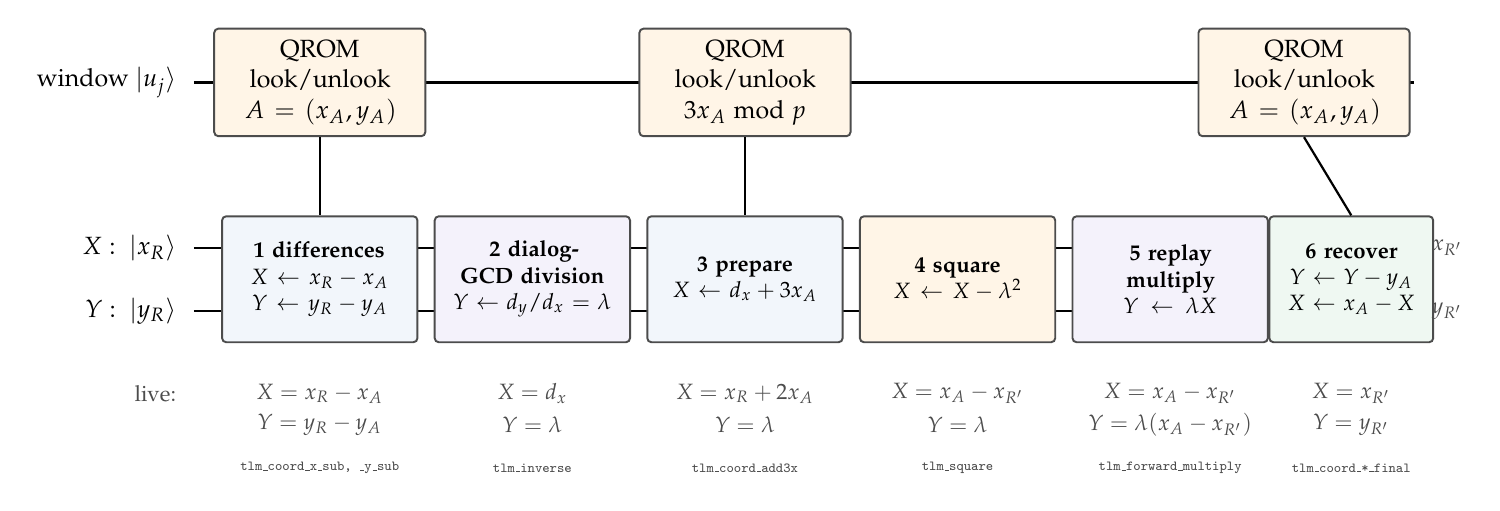
\begin{tikzpicture}[x=1cm,y=1cm,font=\small]
  % buses
  \node[anchor=east] at (0.2,3.4) {window $\ket{u_j}$};
  \draw[wire] (0.3,3.4) -- (15.8,3.4);
  \node[anchor=east] at (0.2,1.3) {$X:\ \ket{x_R}$};
  \node[anchor=east] at (0.2,0.5) {$Y:\ \ket{y_R}$};
  \draw[wire] (0.3,1.3) -- (15.8,1.3); \draw[wire] (0.3,0.5) -- (15.8,0.5);
  \node[blko,text width=24mm] (QA) at (1.9,3.4) {QROM look/unlook\\$A=(x_A,y_A)$};
  \node[blko,text width=24mm] (Q3) at (7.3,3.4) {QROM look/unlook\\$3x_A\bmod p$};
  \node[blko,text width=24mm] (QB) at (14.4,3.4) {QROM look/unlook\\$A=(x_A,y_A)$};
  \node[stage,text width=22mm,minimum height=16mm] (S1) at (1.9,0.9) {\textbf{1 differences}\\$X\gets x_R-x_A$\\$Y\gets y_R-y_A$};
  \node[stage,fill=addviolet,text width=22mm,minimum height=16mm] (S2) at (4.6,0.9) {\textbf{2 dialog-GCD division}\\$Y\gets d_y/d_x=\lambda$};
  \node[stage,text width=22mm,minimum height=16mm] (S3) at (7.3,0.9) {\textbf{3 prepare}\\$X\gets d_x+3x_A$};
  \node[stage,fill=lookorange,text width=22mm,minimum height=16mm] (S4) at (10.0,0.9) {\textbf{4 square}\\$X\gets X-\lambda^2$};
  \node[stage,fill=addviolet,text width=22mm,minimum height=16mm] (S5) at (12.7,0.9) {\textbf{5 replay multiply}\\$Y\gets\lambda X$};
  \node[stage,fill=outgreen,text width=18mm,minimum height=16mm] (S6) at (15.0,0.9) {\textbf{6 recover}\\$Y\gets Y-y_A$\\$X\gets x_A-X$};
  \draw[wire] (QA.south) -- (S1.north); \draw[wire] (Q3.south) -- (S3.north); \draw[wire] (QB.south) -- (S6.north);
  \node[note,anchor=west] at (15.9,1.3) {$x_{R'}$}; \node[note,anchor=west] at (15.9,0.5) {$y_{R'}$};
  % live state
  \foreach \x/\a/\b in {1.9/{x_R-x_A}/{y_R-y_A},4.6/{d_x}/{\lambda},7.3/{x_R+2x_A}/{\lambda},10.0/{x_A-x_{R'}}/{\lambda},12.7/{x_A-x_{R'}}/{\lambda(x_A-x_{R'})},15.0/{x_{R'}}/{y_{R'}}}{
     \node[note] at (\x,-0.55) {$X=\a$}; \node[note] at (\x,-0.95) {$Y=\b$};}
  \node[note,anchor=east] at (0.2,-0.55) {live:};
  % source names
  \foreach \x/\s in {1.9/{tlm\_coord\_x\_sub, \_y\_sub},4.6/{tlm\_inverse},7.3/{tlm\_coord\_add3x},10.0/{tlm\_square},12.7/{tlm\_forward\_multiply},15.0/{tlm\_coord\_*\_final}}{
     \node[note,font=\tiny\ttfamily] at (\x,-1.5) {\s};}
\end{tikzpicture}}
\caption{The six source-level stages of \code{8e9c9a2} and the live contents of the two coordinate registers after each (Supplemental Note~D). In the challenge, $x_A,y_A$ are classical bits; the QROM boxes are what a windowed Shor circuit must add (\cref{sec:windowed}). Stages 2 and 5 are the same Jump-2 dialog-GCD engine run in the ``inverse'' and ``forward'' directions.}
\label{fig:pipeline}
\end{figure}

\paragraph{Nine families.} Supplemental Note~B classifies the $400$ scored source commits of the public competition (to 26~July) into nine optimisation families, six of which have classical-compiler names and three of which are specifically reversible: \emph{windowing}, \emph{algorithmic substitution}, \emph{dead-code and redundancy elimination}, \emph{register and scratch allocation}, \emph{codec/encoding}, \emph{fusion}, \emph{strength reduction}, \emph{constant propagation / classical specialisation}, and \emph{uncompute strategy} \cite{ecdsafail26}. \Cref{tab:census} gives the counts and the share of the realised score reduction each family receives in the paper's bookkeeping. Because the taxonomy is organised by \emph{what a commit did}, while a reader wants to know \emph{how the circuit works}, the rest of this section is organised by circuit component instead---inversion, arithmetic, qubits, uncomputation, post-passes, windowing---and names the family of each lever as it comes up.

\begin{table}[H]
\centering\footnotesize
\begin{tabular}{@{}p{4.1cm}rrrp{6.2cm}@{}}
\toprule
family & commits & \% & $\Delta$ share & typical levers\\
\midrule
dead-code / redundancy elimination & 244 & 61.0 & 39\% & width truncation (149), iteration/threshold tuning (37), fold/carry truncation (37), dead-gate strips (21)\\
register and scratch allocation & 50 & 12.5 & 21\% & ancilla-lifetime / venting (30), scratch reuse (17), in-place mutation (3)\\
uncompute strategy & 22 & 5.5 & 8\% & measurement-based uncompute (all 22)\\
constant propagation / classical specialisation & 19 & 4.8 & $\approx0$ & classical $3x_A$, $(2-q)x_A$, forced-branch prefixes, SAT-proven rows\\
strength reduction & 14 & 3.5 & -- & fast-adder reroute (9), Solinas/NAF folds (5)\\
fusion & 12 & 3.0 & 18\% & gate/op fusion (7), boundary cswap-merge (5)\\
windowing & 8 & 2.0 & 13\% & the Jump-2 inversion base, windowed Solinas shift\\
codec / encoding & 7 & 1.8 & $\approx0$ & base-5 / K5 transcript codecs (low-$Q$ branch)\\
algorithmic substitution & 2 & 0.5 & small & Karatsuba squarer swaps\\
\midrule
verifier search (nonce rerolls) and other & 22 & 5.5 & -- & identity-tail nonce changes, padding\\
\bottomrule
\end{tabular}
\caption{The census of the $400$ scored competition commits to 26~July 2026 (Supplemental Notes~B and C of \cite{ecdsafail26}). ``$\Delta$ share'' is the fraction of the gross frontier reduction attributed to the $69$ largest improvements that a family receives; the four structural families (allocation, fusion, windowing, uncompute) take $\approx60\%$ of it across only $26$ commits, whereas dead-code elimination is frequent but incremental. The wiki's diff-level re-audit of the $180$ later commits (to 7~Oct.) adds a change-type ``inversion/division algorithm swap'' for the three architecture changes of \cref{sec:inversions} \cite{ecdsafail-wiki}.}
\label{tab:census}
\end{table}

\subsection{Six ways to divide: the inversion architectures}\label{sec:inversions}

Every frontier circuit computes $\lambda=d_y/d_x$ and later multiplies by $x_A-x_{R'}$ with a \emph{binary extended-Euclidean walk} of one kind or another; the choice of walk is the single biggest determinant of both $Q$ and $T$, and the competition replaced it five times (\cref{tab:inversions}). The common skeleton is: (i) a forward walk on the pair $(u,v)=(p,\,d)$ that drives it to $(1,0)$ or to a fixed point, recording its branch decisions coherently (they depend on the superposed $d$ and cannot be measured); (ii) a \emph{replay} of the same decisions as linear updates on a coefficient pair seeded with the numerator, which turns $y$ into $y\cdot d^{-1}$ (division) or $y\cdot d$ (multiplication, replay in the opposite direction); (iii) a backward walk that consumes the record and restores $d$. Only the walk rule, what is recorded, and how the record is stored differ.

\begin{table}[H]
\centering\scriptsize
\setlength{\tabcolsep}{3pt}
\begin{tabular}{@{}p{2.1cm}p{2.5cm}p{2.5cm}p{2.7cm}p{2.5cm}p{3.2cm}@{}}
\toprule
& Kaliski & dialog GCD & TrailMix Jump-2 & ping-pong & Skywalk / Leapfrog\\
\midrule
dates (frontier) & 29 May--2 Jun & 2--19 Jun & 19 Jun--21 Aug & 21 Aug--29 Sep & 29 Sep--7 Oct / 7 Oct--\\
rule & qrisp/HJNRS almost-inverse & Stein's binary GCD & Stein, two halvings per step & fixed alternation, no compare & Stein, even rail halves / 3 add-halves + barrel\\
coefficients & $(r,s)$ carried live & replayed from record & replayed, fused into walks & replayed, fused & replayed, fused\\
record per step & $3$ bits ($f,a,b$) & $2$ bits ($b_0,b_0b_1$) & $5$ symbols in $7$ qubits/$3$ steps & $1$ sign bit & trit ($1.6$ q) / $5$ qubits\\
steps per walk & $\approx 397$--$404$ & $399\to259$ (K=2) & $258$--$261$ & $\approx700$ & $\approx393$ / $139$\\
$(Q,T)$ at hand-over & $2006\times2.55$M & $1168\times1.43$M & $1150\times1.285$M & $1250\times0.889$M & $1174\times0.945$M / $1244\times0.798$M\\
\bottomrule
\end{tabular}
\caption{The inversion architectures that held the \ecdsafail{} frontier, in order; dates and operating points from the wiki's concept pages and the 7~Oct.\ leaderboard snapshot \cite{ecdsafail-wiki}.}
\label{tab:inversions}
\end{table}

\subsubsection{Kaliski's almost-inverse (the baseline, 29 May--2 June)}

The organisers' reference circuit ($2{,}715$ qubits, $3{,}942{,}753$ Toffolis unpadded) computed $\lambda$ with two runs of the reversible Kaliski/Montgomery almost-inverse in the form of H\"aner et al.\ \cite{hjnrs20}: state $(u,v_w,r,s)$ initialised to $(p,d_x,0,1)$, a termination flag $f$, one history qubit per iteration, and the straight-line iteration (qrisp step numbers)
\begin{center}\small
\begin{tabular}{@{}ll@{}}
STEP 0 & $\mathit{is\_zero}=[v_w=0]$ (an OR chain); $m_i\mathrel{\oplus}=f\cdot\mathit{is\_zero}$; $f\mathrel{\oplus}=m_i$\\
STEP 1--2 & branch flags $a_f,b_f$ from $u_0,v_{w,0}$ and $\ell=[u>v_w]$\\
STEP 3 & cswap$(a_f)$: $(u,v_w)$ and $(r,s)$\\
STEP 4 & $\mathit{add}_f=f\wedge\neg b_f$; $v_w\mathrel{-}=\mathit{add}_f\cdot u$; $s\mathrel{+}=\mathit{add}_f\cdot r$\\
STEP 6--8 & $v_w\gets v_w/2$ (free relabel); $r\gets 2r\bmod p$\\
STEP 9--10 & cswap$(a_f)$ back; $a_f\mathrel{\oplus}=\neg s_0$
\end{tabular}
\end{center}
run a fixed number of times, then backwards, with $2^{\text{iters}}$ removed by modular halvings. The Kaliski era already contains four of the recurring moves in embryo \cite{ecdsafail-wiki}: \textbf{boundary cswap merges} (STEP 9 of iteration $k$ and STEP 3 of $k+1$ swap the same registers and $\mathrm{cswap}(a)\,\mathrm{cswap}(b)=\mathrm{cswap}(a\oplus b)$, so one width-$n$ Fredkin row is deleted per iteration at the cost of a one-qubit ``frame'' carrying $a_k$ across the boundary: $-274{,}327$ and $-260{,}517$ Toffolis for the two channels), \textbf{in-place $v$ with borrowed carries} (use the live $x$ register as $v_w$, and take the adders' carry ancillas from history slots that are provably still $\ket0$: $2{,}708\to2{,}310$ qubits), \textbf{width truncation} (an envelope fitted to $80{,}000$ sample inputs clips every operation to the bits that can be non-zero at iteration $i$, worth $\approx4{,}300$ Toffolis per margin bit), and \textbf{carry-tail truncation} (above the top set bit of $c=2^{32}+977$ a carry can only propagate, so the chain is cut at $33+W$). By 2~June the frontier stood at $2{,}006\times2{,}552{,}687$, and then the whole inverter was replaced.

\begin{figure}[H]
\centering
\begin{quantikz}[column sep=5pt,row sep=4pt,font=\small]
\lstick{$a_k$}      & \ctrl{1}            & \ctrl{2} & \ctrl{1} &                 &  \\
\lstick{$u$}        & \swap{1}            &          & \swap{1} & \gate[2]{\text{iteration }k{+}1} & \\
\lstick{$v_w$}      & \targX{}            &          & \targX{} &                 & \\
\end{quantikz}
\hspace{4mm}$\Longrightarrow$\hspace{4mm}
\begin{quantikz}[column sep=5pt,row sep=4pt,font=\small]
\lstick{$a_k$}         & \ctrl{3}  &          &  & & \\
\lstick{$a_{k+1}$}     &           & \ctrl{2} & \ctrl{2}   &  & \\
\lstick{$u$}           &           &          & \swap{1} & \gate[2]{\text{iteration }k{+}1} & \\
\lstick{$v_w$}         & \targ{}   & \targ{}  & \targX{} & & \\
\end{quantikz}
\caption{Boundary cswap-merge (fusion family). Left: the step-9 un-swap of iteration $k$ and the step-3 swap of iteration $k+1$ act on the same pair. Right: the identity $\mathrm{cswap}(a_k)\mathrm{cswap}(a_{k+1})=\mathrm{cswap}(a_k\oplus a_{k+1})$ replaces two width-$n$ Fredkin rows ($2n$ Toffolis) by one row driven by a parity formed with a free CNOT into a one-qubit frame (shown schematically; the frame qubit is cleared at the boundary that set it, so it is never live at the step-4 peak). Commits \code{d35d6e7}/\code{9bcc27d} and \code{36a2989}/\code{112d5a4} \cite{ecdsafail26,ecdsafail-wiki}.}
\label{fig:cswap-merge}
\end{figure}

\subsubsection{The dialog GCD: record the walk, replay it (2--19 June)}\label{sec:dialog}

Schrottenloher's construction \cite{schrottenloher26} (following the ``record and replay'' idea of \cite{khattar25}) drops the B\'ezout coefficients from the walk altogether. Run Stein's binary GCD on $(u,v)=(p,a)$ alone,
\begin{equation}\label{eq:dialog-step}
b_0\gets v_0;\qquad b_{01}\gets b_0\wedge[u>v];\qquad \text{if } b_{01}:\ \mathrm{swap}(u,v);\qquad \text{if } b_0:\ v\gets v-u;\qquad v\gets v/2 ,
\end{equation}
and keep only the two decision bits per step---the \emph{dialog}. Each step is a linear map $M_i$ on $(u,v)$; the product $M=M_L\cdots M_1$ sends $(p,a)\mapsto(1,0)$. Over $\F_p$ the constant $p$ is $0$, so replaying the same decisions on the pair $(0,y)$ gives $(y/a,\,0)$: \emph{the record of the walk on $a$ is a program for dividing by $a$}, and the identical program read in the other direction (doublings instead of halvings) multiplies by $a$. The replay of one step is
\[
\mathrm{cswap}(b_{01},x,y);\qquad y\gets y-b_0\,x \bmod p;\qquad y\gets y/2\bmod p ,
\]
so the only quantum data it touches are the two coefficient registers and the two recorded bits; it never looks at $a$ again. Since $(b_0,b_{01})=(0,1)$ cannot occur, three steps carry $3^3=27<32$ states and fit in five qubits instead of six, giving an asymptotic $2.355n$ qubits for the record in place of $2n$ for $(r,s)$---and, unlike the Kaliski design, the record is only consumed at the very end, so its lifetime is the whole circuit, which is what the later codecs and the register-sharing of \cref{sec:regshare} address. The first dialog submission, \code{cddd5df} (2~June, $1{,}698\times2{,}447{,}846$), replaced both inversions at once; by 18~June (\code{ba3efc1}) the route stood at $1{,}168\times1{,}431{,}621$, almost entirely by tuning its truncations: step count ($399\to393$, then $259$ under K=2), the width envelope $\mathrm{active\_width}(s)=\lceil 256-s\cdot\mathrm{slope}+\mathrm{margin}\rceil_{\mathrm{even}}$ with slope $0.7075\to1.017$ and margin $37\to10$, per-step compare widths from a baked table of observed maxima of $w-\mathrm{msb}(u\oplus v)$, body trims, apply-pass chunking, and fold windows \cite{ecdsafail-wiki}.

\begin{figure}[H]
\centering
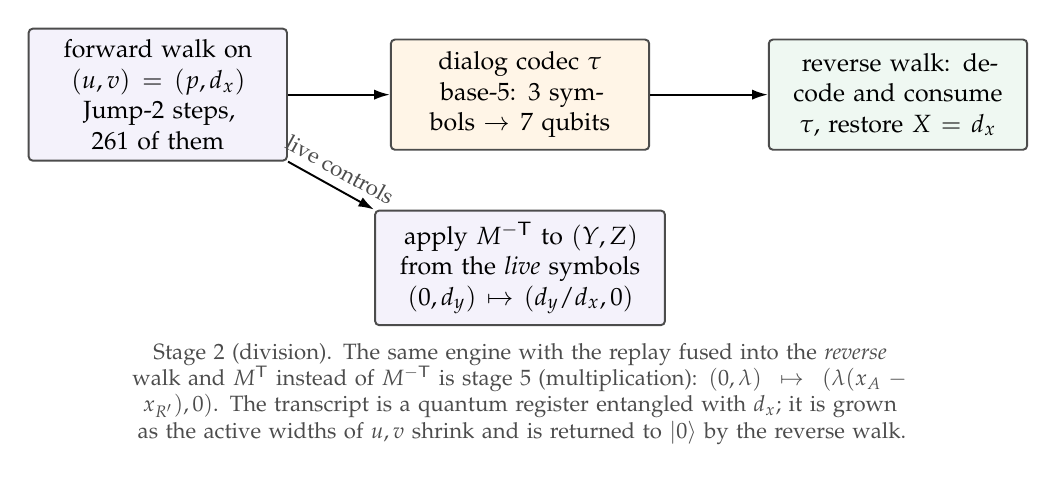
\begin{tikzpicture}[x=1cm,y=1cm,font=\small]
  \node[blkv,text width=30mm,minimum height=14mm] (W) at (0,2.2) {forward walk on $(u,v)=(p,d_x)$\\ Jump-2 steps, $261$ of them};
  \node[blko,text width=30mm,minimum height=14mm] (C) at (4.6,2.2) {dialog codec $\tau$\\ base-5: $3$ symbols $\to7$ qubits};
  \node[blkv,text width=34mm,minimum height=14mm] (A) at (4.6,0) {apply $M^{-\mathsf T}$ to $(Y,Z)$ from the \emph{live} symbols\\ $(0,d_y)\mapsto(d_y/d_x,0)$};
  \node[blkg,text width=30mm,minimum height=14mm] (R) at (9.4,2.2) {reverse walk: decode and consume $\tau$, restore $X=d_x$};
  \draw[flow] (W) -- (C); \draw[flow] (C) -- (R); \draw[flow] (W.south east) -- node[note,above,sloped]{live controls} (A.north west);
  \node[note,text width=12cm] at (4.6,-1.6) {Stage 2 (division). The same engine with the replay fused into the \emph{reverse} walk and $M^{\mathsf T}$ instead of $M^{-\mathsf T}$ is stage 5 (multiplication): $(0,\lambda)\mapsto(\lambda(x_A-x_{R'}),0)$. The transcript is a quantum register entangled with $d_x$; it is grown as the active widths of $u,v$ shrink and is returned to $\ket0$ by the reverse walk.};
\end{tikzpicture}
\caption{Dialog-GCD division as implemented in \code{8e9c9a2} (Supplemental Note~D, pp.\,7 and 14 redrawn). Every halving, swap and subtraction of the walk is a linear update $M$ of $(u,v)$; the same controls apply the coefficient update $M^{-\mathsf T}$ to the pair $(Y,Z)$, so while the walk reduces $(p,d_x)\to(1,0)$ the numerator $d_y$ becomes $d_yd_x^{-1}=\lambda$.}
\label{fig:dialog}
\end{figure}

\subsubsection{Jump-2 and the base-5 codec (TrailMix, 19 June--21 August)}\label{sec:jump2}

Trail of Bits' ``TrailMix'' port \cite{ecdsafail26} (submission \code{bdb1d22}) reorders the step so that the halving comes first and allows a \emph{second} halving when the first leaves $v$ even:
\begin{equation}\label{eq:jump2}
\begin{aligned}
&v\gets v/2;\qquad s_2=[v\text{ even}];\qquad \text{if } s_2:\ v\gets v/2;\qquad b=v_0;\\
&s=b\wedge[v<u]_{\text{top }k\text{ bits}};\qquad \text{if } s:\ \mathrm{swap}(u,v);\qquad \text{if } b:\ v\gets v-u .
\end{aligned}
\end{equation}
Every macro-step ends with $v$ even (the subtraction of odd $u$ from odd $v$ is even; if $b=0$, $v$ was even already), so the next unconditional halving is always valid: Jump-2 is an \emph{exact retiming} of the binary GCD that makes about $0.95$ bits of progress per recorded symbol instead of $0.71$, which is why the fixed budget fell from $393$ to $258$--$261$ macro-steps (non-convergence $2.839\times10^{-4}$ at $258$, $2.86\times10^{-5}$ at $261$ over $10^7$ inputs). The symbol $\sigma=(b,s,s_2)$ has three bits but only five reachable values---$s_2=0\Rightarrow b=1$ and $b=0\Rightarrow s=0$---so it is a base-5 digit $d=\phi(\sigma)\in\{0,\dots,4\}$, and three digits pack as $z=d_0+5d_1+25d_2\le124<2^7$: seven qubits for nine raw bits, by a reversible permutation of basis states (no decision is measured or discarded). For $261$ symbols the tape is $2+86\cdot7+5=609$ qubits instead of $783$ (\cref{fig:codec}). The windowing family's largest entry is exactly this re-blocking of the Euclidean loop (its landing is the competition's second-largest single frontier move), and the codec family is its storage \cite{ecdsafail26}.

\begin{figure}[H]
\centering
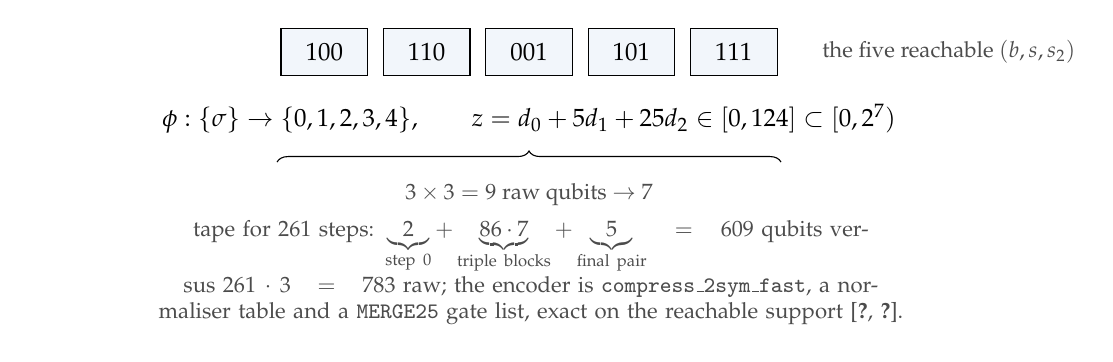
\begin{tikzpicture}[x=1cm,y=1cm,font=\small]
  \foreach \x/\s in {0/{100},1.3/{110},2.6/{001},3.9/{101},5.2/{111}} {\node[draw,fill=gateblue,minimum width=11mm,minimum height=6mm] at (\x,2.6) {$\s$};}
  \node[note,anchor=west] at (6.2,2.6) {the five reachable $(b,s,s_2)$};
  \node at (2.6,1.75) {$\phi:\{\sigma\}\to\{0,1,2,3,4\},\qquad z=d_0+5d_1+25d_2\in[0,124]\subset[0,2^7)$};
  \draw[decorate,decoration={brace,amplitude=4pt}] (-0.6,1.2) -- (5.8,1.2) node[midway,below=4pt,note]{$3\times3=9$ raw qubits $\to$ $7$};
  \node[note,text width=12.5cm] at (2.6,-0.2) {tape for $261$ steps: $\underbrace{2}_{\text{step 0}}+\underbrace{86\cdot 7}_{\text{triple blocks}}+\underbrace{5}_{\text{final pair}}=609$ qubits versus $261\cdot3=783$ raw; the encoder is \code{compress\_2sym\_fast}, a normaliser table and a \code{MERGE25} gate list, exact on the reachable support \cite{ecdsafail-supp,ecdsafail-wiki}.};
\end{tikzpicture}
\caption{The base-5 transcript codec of the Jump-2 route (codec/encoding family; Supplemental Note~D, p.\,9). In the earlier June route the same idea appeared as the K2-pair ($6\to5$), K5 ($15\to12$), head-11 and tail-3 block codecs \cite{ecdsafail-wiki}.}
\label{fig:codec}
\end{figure}

\paragraph{Width scheduling.} The walk operates on shrinking registers: at step $i$ only the active $w_i=\code{SCHED\_J2}[i]$ low bits of $u,v$ are touched, the comparator looks only at $\code{GAP\_J2}[i]$ top bits, and the freed high lanes host the growing tape. Note~D's live-width model for stage 2,
\begin{equation}\label{eq:livewidth}
Q_i\approx\underbrace{512}_{\text{B\'ezout pair}}+\underbrace{|\tau_i|}_{\text{compressed dialog}}+\underbrace{2w_i}_{u_i,v_i}+\underbrace{q_{\mathrm{work},i}}_{\text{compare, carry, control}},
\end{equation}
states the scheduling objective: make the decrease of $2w_i$ absorb the growth of $|\tau_i|$, while hosting and measurement-based cleanup keep $q_{\mathrm{work},i}$ below the same peak. The known bits $u_0=1$ and $v_0=0$ are ``parked'' while dormant and their lanes lent out; chunked adders borrow already-live registers as dirty vent space; every borrowed value is restored before its owner is active again.

\subsubsection{Ping-pong: fixed-depth signed binary division (21 August--29 September)}\label{sec:pingpong}

Submission \code{897dda2} (teddyjfpender) replaced the GCD by a divider that needs no comparison at all. Two \emph{odd signed} registers in a $259$-bit two's-complement envelope take turns being halved in a fixed order:
\begin{equation}\label{eq:pingpong}
\mathrm{sign}=\mathrm{target}_1\oplus\mathrm{source}_1,\qquad \mathrm{target}\gets\frac{\mathrm{target}+(-1)^{\mathrm{sign}}\,\mathrm{source}}{2},
\end{equation}
where the sign is chosen so that the sum is $\equiv2\pmod4$ and the result is odd again; roles alternate with the round parity, which is known at build time, so no data-dependent swap is needed. The pair $(u,v)=(p,d)$ converges to a fixed point $(\pm1,\pm1)$; one tape qubit per round records the sign; the replay runs the same signed halvings modulo $p$ on $(\mathrm{coefficient},\mathrm{numerator})=(0,c)$ and ends at $(\pm c/a,\pm c/a)$, after which the terminal signs make the two registers equal and a row of CNOTs clears one of them. Each replay round is one fused cell: a chunked add with measured boundary carries, a fold by one of $\{-f,0,+f,+2f\}$ with $f=2^{32}+977$ restricted to a window, and a measured overflow flag repaired by a truncated compare. The walk is cheaper per round ($257$ Toffolis in Julian's reconstruction, \cref{sec:shor-impl}) but takes $\approx700$ rounds, and its $700$-bit tape sets the peak: the memory note's plateau is
\[
700\ (\text{tape})+256+256\ (\text{coefficient pair})+2\ (\text{terminal signs})+86\ (\text{chunk carry ladder})=1{,}300 ,
\]
which the follow-ups brought down to $1{,}250$ by lending the $16$ known terminal wires (the sign copies in bits $1..7$ of each $9$-wire register and the constant bit $0$), interleaving the replay with the walk so that early replay rounds share the machine with only part of the tape, and sizing every carry ladder against a peak cap (\code{PP\_WALK\_MAX\_QUBITS}) \cite{ecdsafail-wiki}. Against the TrailMix frontier the swap cost $171$ qubits and saved $332$k Toffolis ($1{,}321\times952{,}707$ against $1{,}150\times1{,}284{,}776$), the largest single score delta of the extension census.

\subsubsection{Skywalk: Stein's GCD with a trit history (29 September--7 October)}\label{sec:skywalk}

\code{8ee337c} (mochimodev) returned to Stein's rule but removed its comparison by a change of representation: keep the pair as the unordered magnitudes $\{u+v,u\}$, exactly one of which is even; call it $E$ and the other $O$; the next state is $\{E/2,|O-E/2|\}$. One \emph{rail tick} is
\begin{enumerate}[nosep]
\item $c=R_1[0]$; Fredkin-swap $R_1[i]\leftrightarrow R_2[i]$ on $c$ for $i\ge1$ and $R_2[0]\mathrel{\oplus}=c$, so that the even rail is in $R_1$;
\item $E/2=R_1[1..]$ is a relabelling (no gates);
\item $R_2\gets R_2\mp E/2$, subtracting when the signs agree (signs are kept, not absolute values);
\item the wire $c$ leaves the rail as the tape's orientation bit $\mathrm{typ}_t=\mathrm{typ}_{t-1}\oplus c_t$, and the add's sign-flip wire becomes $s_t$.
\end{enumerate}
The pair $(\mathrm{typ},s)$ takes three legal values, a \emph{trit}, and five trits pack into eight qubits ($3^5=243\le256$), i.e.\ $1.6$ qubits per tick; about $393$ ticks suffice where ping-pong needed $\approx700$, so the history is shorter and $Q$ fell $1{,}250\to1{,}174$, while $T$ rose $6.4\%$ because every tick pays a full-width Fredkin row on the rails and every payload cell a conditional $256$-bit route swap \cite{ecdsafail-wiki}. The payload is carried as a sum/difference (``butterfly'') pair $(\Sigma,\Delta)$ with the division cell $\Sigma\gets(\Sigma-(-1)^{g}\Delta)/2\bmod p$, $g=\mathrm{typ}_t$, followed by a swap if $s$; seeded with $(2N,0)$ it parks at $\Sigma=\Delta=N/d$, so the endpoint $\Delta\mathrel{\oplus}=\Sigma$ costs no Toffoli.

\subsubsection{Leapfrog: a route-free multi-step 2-adic walk (from 7 October)}\label{sec:leapfrog}

\code{86221ad} (BitWonka) makes much bigger steps. Two odd rails $R_0,R_1$ in two's complement; at tick $t$ the target $T=R_{t\bmod2}$ is updated from the source $B=R_{1-t\bmod2}$ by
\begin{enumerate}[nosep]
\item two \emph{forced} add-halves, letters $s_0,s_1$: $T\gets(T+(-1)^sB)/2$ with $s=T_1\oplus B_1$ (so the sum is $\equiv2\bmod4$ and $T$ stays odd; the sign costs two CNOTs);
\item one \emph{choice} add-halve, letter $s_3$: of $T\pm B$, exactly one is $\equiv0\bmod4$ (the \emph{deep} candidate $D$); take it when $D\bmod32\neq0$ (so its extra zeros $e=v_2(D)-1\le3$) and the step is not the rail-growing ``$e=1$ with equal signs'' case (rule \emph{sign2}); with \code{LF\_W1} the excluded case is reopened when $|T|>4|B|$ on a $K$-bit window of the top bits;
\item a \emph{barrel}, letters $k_1=e\,\&\,1$, $k_2=e\gg1$: an arithmetic right shift of the rail by $e$ (the $e$ known-zero low wires rotate to the top and are sign-filled, $1.5w-2$ Toffolis) and, on the payload, a controlled multiplication by $2^{-e}\bmod p$: with $m=P\bmod 2^e$ and $f-1\equiv0\bmod16$, $P\cdot2^{-e}\equiv\mathrm{rotr}_e\big(P-m(f-1)\big)$---one fold ladder whose addend bits are AND-monomials of the three bits of $m$, then a rotation \code{rot4} built from three controlled reflections ($1.5n-2$ Fredkins).
\end{enumerate}
Each tick removes $3+e$ low bits of the target, so $139$ ticks suffice (Skywalk $\approx393$, ping-pong $\approx700$); the letter is five raw qubits with no codec ($695$ tape qubits), the payload work per tick is three replay cells and one barrel ($\approx556$ cell-equivalents per pass against Skywalk's $393$ cells $+393$ route swaps), and because the target is fixed by the tick's parity there is no routing at all. The width envelope (\code{env\_w1\_peel139.txt}) is a greedy \emph{peeling} fit over $1.92$\,M walks that drops the walks that never park and then repeatedly lowers whichever position saves the most priced Toffoli per walk sacrificed; the author reports $\lambda=14.4\pm0.4$ under the inherited $19.5$ cap. The landing went $1{,}172\times945{,}335\to1{,}243\times804{,}160$ ($999{,}570{,}880$, the first score below $10^9$), and three same-day follow-ups reached $1{,}244\times797{,}905$ \cite{ecdsafail-wiki}. The repository head on 11~October (\code{c672dda}) still runs Leapfrog, with walk caps of $1{,}235$--$1{,}237$ in its ``spookyfrog'' recipe variants \cite{ecdsafail-repo}.

\begin{figure}[H]
\centering
\resizebox{\textwidth}{!}{%
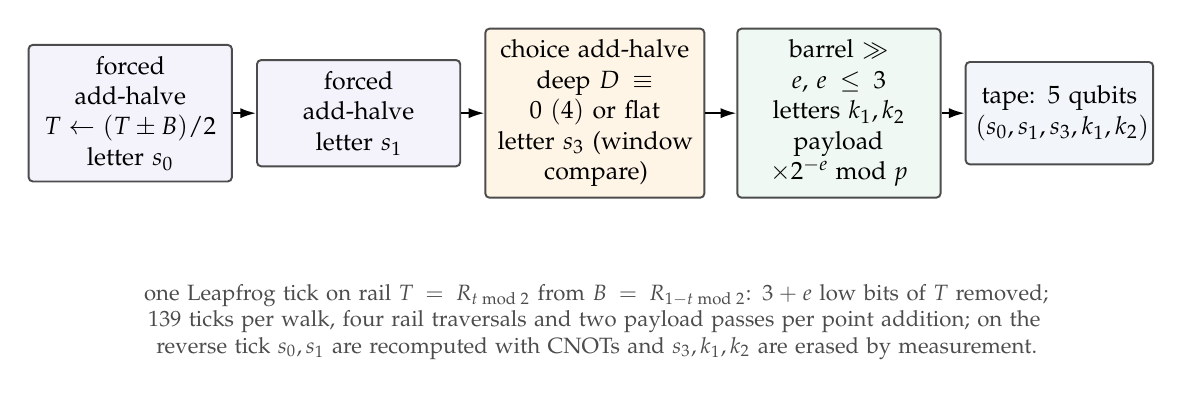
\begin{tikzpicture}[x=1cm,y=1cm,font=\footnotesize]
  \node[blkv,text width=23mm,minimum height=13mm] (a) at (0,0) {forced add-halve\\$T\gets(T\pm B)/2$\\letter $s_0$};
  \node[blkv,text width=23mm,minimum height=13mm] (b) at (2.9,0) {forced add-halve\\letter $s_1$};
  \node[blko,text width=25mm,minimum height=13mm] (c) at (5.9,0) {choice add-halve\\deep $D\equiv0\ (4)$ or flat\\letter $s_3$ (window compare)};
  \node[blkg,text width=23mm,minimum height=13mm] (d) at (9.0,0) {barrel $\gg e$, $e\le3$\\letters $k_1,k_2$\\payload $\times2^{-e}\bmod p$};
  \node[blk,text width=21mm,minimum height=13mm] (e) at (11.8,0) {tape: $5$ qubits\\$(s_0,s_1,s_3,k_1,k_2)$};
  \draw[flow] (a)--(b); \draw[flow] (b)--(c); \draw[flow] (c)--(d); \draw[flow] (d)--(e);
  \node[note,text width=12.5cm,anchor=north] at (5.9,-2.05) {one Leapfrog tick on rail $T=R_{t\bmod2}$ from $B=R_{1-t\bmod 2}$: $3+e$ low bits of $T$ removed; $139$ ticks per walk, four rail traversals and two payload passes per point addition; on the reverse tick $s_0,s_1$ are recomputed with CNOTs and $s_3,k_1,k_2$ are erased by measurement.};
\end{tikzpicture}}
\caption{The Leapfrog tick (\cite{ecdsafail-wiki}, concept page \emph{leapfrog}).}
\label{fig:leapfrog}
\end{figure}

\begin{keybox}[title={Why the walks matter for fault tolerance}]
A point addition is four rail traversals and two payload passes of a sequential walk; the walk's steps are \emph{inherently serial} (each depends on the previous one) and are built from ripple adders. In the challenge metric only the Toffoli count is priced, but on a fault-tolerant machine the \emph{depth} is what the reaction time multiplies (\cref{sec:physical}): Julian's measurements in \cref{sec:shor-impl} put the Toffoli depth of a point addition at $0.8$--$0.95\times$ its Toffoli count for every ripple-based construction. Fewer, fatter steps (Leapfrog) therefore also shorten the critical path.
\end{keybox}

\subsection{The arithmetic layer: where the Toffolis are}\label{sec:arith}

Almost every Toffoli in any of these circuits sits inside a ripple-carry adder, and the levers of the \emph{strength reduction}, \emph{fusion}, \emph{dead-code} and \emph{uncompute} families mostly act there. The building blocks, in the order they were introduced into the frontier:

\subsubsection{Temporary-AND adders, Cuccaro bridges, and the carry trade}\label{sec:adders}

The frontier's register-plus-register adder is Gidney's temporary-logical-AND ripple adder \cite{gidney18add}: at position $i$ the carry is $c_{i}=\MAJ(a_i,b_i,c_{i-1})$, computed by folding the previous carry into both operands with two CNOTs, writing the AND into a \emph{fresh} wire with one Toffoli and XOR-ing the previous carry in. When the sum is done, each carry wire is erased with $\Hmr$ and a classically-conditioned CZ on the two operands---zero Toffolis (\cref{sec:mbu}). The textbook Cuccaro adder \cite{cuccaro04} keeps the carry inside the operand (MAJ then UMA) at $\approx2n$ Toffolis and one ancilla. The two sit at opposite ends of one trade:
\begin{center}\small
\begin{tabular}{@{}lcc@{}}
\toprule
$n$-bit adder & Toffolis & owned carry wires\\
\midrule
temporary-AND ripple, with carry-out (``vented'') & $n$ & $n-1$\\
temporary-AND ripple, wrapped mod $2^n$ & $n-1$ & $n-2$\\
Cuccaro MAJ/UMA & $\approx2n$ & $\approx1$\\
one Cuccaro ``bridge'' stage inside a measured ripple & $+1$ per stage & $-1$ per stage\\
\bottomrule
\end{tabular}
\end{center}
``Bridges'' (\code{bridge.rs}) are single Cuccaro stages spliced into a measured ripple where the live count would otherwise exceed the cap: each trades one extra CCX for one fewer carry wire, and the number of bridges per replay cell is a per-round profile (\code{I35\_PROFILE}) tuned against the peak. For a \emph{classical} addend $c$ the carry out of position $i$ is identically zero below the first position that can generate one, so \code{add\_const} emits $n-2-\mathrm{ctz}(c)$ Toffolis (dead-low carry elision, exact); two call sites can prove the first carry zero and save more \cite{ecdsafail-wiki}.

\begin{figure}[H]
\centering
\begin{quantikz}[column sep=6pt,row sep=5pt,font=\small]
\lstick{$c_{i-1}$} & \ctrl{1} & \ctrl{2} &          & \ctrl{3} & \ \ldots\ &          &          & \ctrl{1}  & \ctrl{2} & \\
\lstick{$a_i$}     & \targ{}  &          & \ctrl{2} &          & \ \ldots\ &          & \ctrl{2} & \targ{}   &          & \\
\lstick{$b_i$}     &          & \targ{}  & \ctrl{1} &          & \ \ldots\ & \gate{\text{sum}} & \control{} &  & \targ{}  & \\
\lstick{$\ket0$}   &          &          & \targ{}  & \targ{}  & \ \ldots\ & \gate{H} & \meter{}\wire[u][1]{c} & \setwiretype{n} & & \\
\end{quantikz}
\caption{One slice of a temporary-AND ripple adder \cite{gidney18add}. Left: $c_i=\MAJ(a_i,b_i,c_{i-1})$ is written into a clean wire with one Toffoli (the AND of the CNOT-modified operands) and one CNOT. Right: once the sum bit has been used, the carry wire is measured in the $X$ basis ($H$ then measure---the challenge's $\Hmr$); outcome $m=1$ leaves the phase $(-1)^{a_i'b_i'}$ on the two controls, which a CZ conditioned on $m$ (the classical wire going up) removes; the CNOTs are then undone. Net: one Toffoli per carry instead of two.}
\label{fig:and-adder}
\end{figure}

\subsubsection{Chunked adders and measured carry erasure}\label{sec:chunked}

A full ladder keeps $\approx n$ carry wires live. When they do not fit under the cap the add is cut into chunks; each chunk unwinds its own carries before the next starts, so only one chunk's ladder is live at a time, and the carry left on the boundary wire between chunks is \emph{erased by measurement and repaired by a comparison}: the carry out of $\mathrm{sum}=\mathrm{acc}+\mathrm{addend}$ is exactly $[\mathrm{sum}<\mathrm{addend}]$, so after $\Hmr$ on the boundary carry, on outcome $1$ a \emph{phase oracle} $(-1)^{[\mathrm{sum}<\mathrm{addend}]}$ computed on the top $k$ bits of the two operands cancels the kickback (\code{compare::erase\_with\_compare}, \code{cmp\_lt\_phase\_conditioned}). If the whole chunk is compared and its carry-in is known the erase is exact; if only the top $k$ bits are compared it is wrong exactly when both operands agree on all $k$ bits, probability $\approx2^{-k}$ per call---and since the oracle runs only on the $m=1$ shots, a comparator bit costs about $0.5$ \emph{executed} Toffolis. Chunking saves qubits and costs Toffolis; moving from two chunks to three is ``a step worth hundreds of Toffoli'' \cite{ecdsafail-wiki}. The same phase-oracle erase clears the modular adder's overflow flag (\code{ERASE\_COMPARE}) and the replay cell's flag (\code{flag\_compare}).

\begin{figure}[H]
\centering
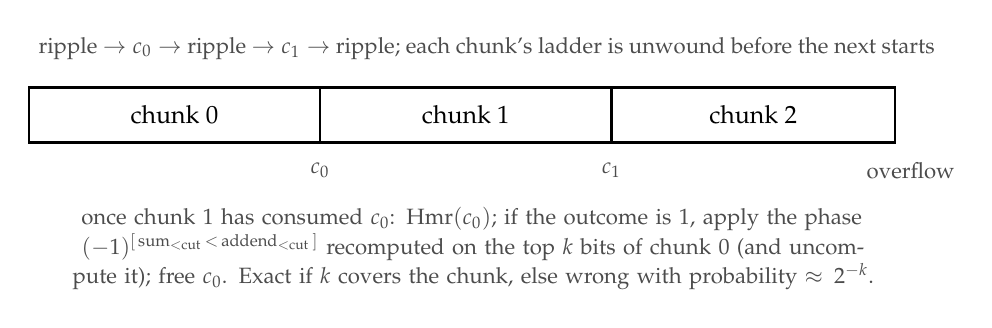
\begin{tikzpicture}[x=1cm,y=1cm,font=\small]
  \draw[wire] (0,0) rectangle (11,0.7);
  \foreach \x in {3.7,7.4} {\draw[wire] (\x,0) -- (\x,0.7);}
  \node at (1.85,0.35) {chunk 0}; \node at (5.55,0.35) {chunk 1}; \node at (9.2,0.35) {chunk 2};
  \node[note] at (3.7,-0.35) {$c_0$}; \node[note] at (7.4,-0.35) {$c_1$}; \node[note] at (11.2,-0.35) {overflow};
  \node[note,anchor=west] at (0,1.2) {ripple $\to c_0\to$ ripple $\to c_1\to$ ripple; each chunk's ladder is unwound before the next starts};
  \node[note,text width=11cm,anchor=north west] at (0,-0.7) {once chunk 1 has consumed $c_0$: $\Hmr(c_0)$; if the outcome is $1$, apply the phase $(-1)^{[\,\mathrm{sum}_{<\mathrm{cut}}\,<\,\mathrm{addend}_{<\mathrm{cut}}\,]}$ recomputed on the top $k$ bits of chunk 0 (and uncompute it); free $c_0$. Exact if $k$ covers the chunk, else wrong with probability $\approx2^{-k}$.};
\end{tikzpicture}
\caption{Chunked addition with measured boundary carries (concept pages \emph{adders-and-carries}, \emph{comparator-and-width-truncation} of \cite{ecdsafail-wiki}).}
\label{fig:chunked}
\end{figure}

\subsubsection{Truncated comparators and width schedules}\label{sec:truncation}

This is the most frequent change-type of the whole competition ($184$ of $584$ accepted commits by the wiki's count). Two cases recur. (a) A comparator that exists only to clean up a carry or flag (above) is narrowed to the top $k$ bits; the error is a top-$k$ tie. (b) A register that provably shrinks during the walk is narrowed round by round: ping-pong's \code{PP\_WIDTH\_SCHEDULE} (``259,258x19,257x5,\dots,8x9,8x2''), TrailMix's \code{SCHED\_J2}/\code{GAP\_J2}, Skywalk's and Leapfrog's envelope files. A trimmed top wire is a CNOT from the wire below it followed by a free---valid only if it was a sign copy. The schedules are \emph{fitted}, not proved: \code{b5796ce} gave each round the smallest width whose violation count stayed within a $\lambda$ budget of about $1.5$ per draw. Per-round \emph{shapes} then equalise the per-site error, since minimising total bits at fixed total error means equal error per site (\code{PP\_CHUNK\_SHAPE} ``64:0,38:1,25:-3,0:-4'', \code{PP\_FLAG\_SHAPE}). Two things distinguish an \emph{exact} truncation (narrowing to a proven-non-zero prefix, e.g.\ the Kaliski invariant $\bitlen u+\bitlen v_w\le2n-i$) from a \emph{probabilistic} one: the former adds no hard inputs; the latter is a ``sell'' of Toffolis for $\lambda$ that must be ``bought'' back somewhere else to stay under the cap \cite{ecdsafail-wiki}.

\subsubsection{Pseudo-Mersenne folds}\label{sec:fold}

Because $p=2^{256}-f$ with $f=2^{32}+977$, $2^{256}\equiv f\pmod p$: anything that spills past bit $256$ is reduced by adding the spill times $f$ into the low bits. A modular add/sub (\code{mod\_addsub}) is: integer add with the top carry vented onto an $\mathit{overflow}$ wire; a constant add of $f$ into the low $fs=33+\code{FOLD\_GUARD}$ bits controlled by that wire; erase the wire with a measured compare. The dropped carry off the top of the window is the whole approximation, with error $\approx2^{-(\code{FOLD\_GUARD}+1)}$ per call (a carry escapes only through $\code{FOLD\_GUARD}+1$ consecutive ones). Narrowing a window is one of the commonest Toffoli levers and the commonest \emph{qubit} lever inside the replay (``the cell's fold is the widest thing alive in the trailing batch''). The replay cell folds by one of $\{-f,0,+f,+2f\}$ selected by the sign, the parity of the sum and the overflow, without building an operand register (\code{fold\_selected}); the square's high limb is folded with $f$ written in non-adjacent form $f=1+2^4-2^6+2^{10}+2^{32}$ (five signed terms, the \emph{signed-digit constant decomposition} of the strength-reduction family) \cite{ecdsafail26,ecdsafail-wiki}.

\subsubsection{Karatsuba squaring with pseudo-Mersenne modulo (stage 4)}\label{sec:square}

Stage 4 computes $X\gets X-\lambda^2$. Writing $\lambda=L+\beta H$ with $\beta=2^{128}$ and $U=L^2$, $V=H^2$, $W=(L+H)^2$,
\begin{equation}\label{eq:karatsuba}
\lambda^2=U+\beta(W-U-V)+\beta^2V\equiv U+\beta(W-U-V)+fV\pmod p ,
\end{equation}
so three half-size squares replace one full square, the $2^{256}V$ limb folds to $fV$, and the five signed terms of $f$ turn $fV$ into shifted additions. Squaring is cheaper than multiplying because the cross products $y_iy_j$ are symmetric (each is needed once) and the diagonal terms $y_i^2=y_i$ cost nothing: the three squares have $24{,}512$ unordered cross products, $24.9\%$ fewer than a direct $256$-bit symmetric square ($32{,}640$). The circuit-level specialisations are what make it cheap (\cref{fig:square}): each of $W,U,V$ is built in a $2|x|$-bit register, its signed contribution is applied straight into $X$, and it is unbuilt before the next is built, so no $512$-bit square is ever live; leaf squares are triangles of add-or-subtract rows selected by $x_i$ (a complement frame, no controlled gates; \code{square\_addsub\_vented}, $-43{,}467$ T at \code{422f21d}); the split recurses while a half is at least $64$--$65$ bits (break-even near $60$ bits by the cost model $B(m)=m(m-1)/2+4m-3$ vs.\ $K(m)=B(a)+B(b)+B(b+1)+a+7b+1$), limited by the qubit peak rather than the Toffoli count \cite{ecdsafail26,ecdsafail-wiki}. The identity is exact; every approximation lives in the fold windows.

\begin{figure}[H]
\centering
\resizebox{\textwidth}{!}{%
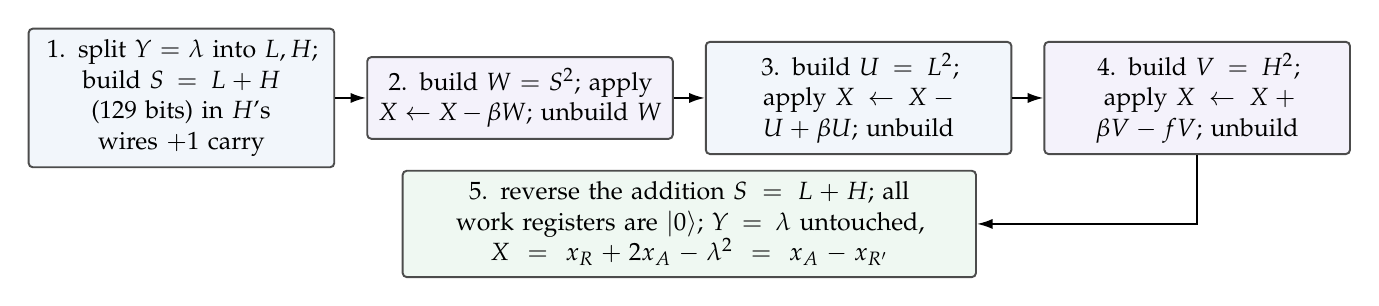
\begin{tikzpicture}[x=1cm,y=1cm,font=\footnotesize]
  \node[blk,text width=36mm] (s1) at (0,0) {1. split $Y=\lambda$ into $L,H$;\\build $S=L+H$ ($129$ bits) in $H$'s wires $+1$ carry};
  \node[blkv,text width=36mm] (s2) at (4.3,0) {2. build $W=S^2$; apply $X\gets X-\beta W$; unbuild $W$};
  \node[blk,text width=36mm] (s3) at (8.6,0) {3. build $U=L^2$; apply $X\gets X-U+\beta U$; unbuild};
  \node[blkv,text width=36mm] (s4) at (12.9,0) {4. build $V=H^2$; apply $X\gets X+\beta V-fV$; unbuild};
  \draw[flow] (s1)--(s2); \draw[flow] (s2)--(s3); \draw[flow] (s3)--(s4);
  \node[blkg,text width=70mm] (s5) at (6.45,-1.6) {5. reverse the addition $S=L+H$; all work registers are $\ket0$; $Y=\lambda$ untouched, $X=x_R+2x_A-\lambda^2=x_A-x_{R'}$};
  \draw[flow] (s4.south) |- (s5.east);
\end{tikzpicture}}
\caption{The build--apply--unbuild schedule of the symmetry-aware streamed Karatsuba square (Supplemental Note~D, p.\,13).}
\label{fig:square}
\end{figure}

\subsubsection{Constants, strength reduction, and fusion}\label{sec:fusion}

\emph{Classical specialisation} (constant propagation family): since $x_A$ is classical, $3x_A\bmod p$ is computed on the host and loaded, so stage 3 is one modular addition instead of two additions, a doubling and a halving (\code{662e267}); the final $x_A-X$ is $\overline X+(x_A+1)$ with the pseudo-Mersenne correction (\cref{fig:pipeline}, stage 6); H\"aner et al.'s $x\mathrel{-}=(2-q)x_2$ is the same idea with a control. A \emph{guaranteed-prefix} specialisation runs the first $304$ Kaliski iterations with a branch-free body because the sum invariant proves they cannot terminate ($-158{,}254$ T, $3.6\%$). \emph{Strength reduction}: inlining the add-$c$/branch/parity pattern of the Solinas reduction into Kaliski's step 8 ($-2{,}090{,}712$ T); $acc-X\equiv acc+(p-X)$ so the cheaper conditional \emph{adder} drives the inner loop ($-256{,}016$ T); Litinski's add-subtract schoolbook rows ($n-1$ instead of $2n-1$ Toffolis per row); rerouting five call sites to the carry-ancilla adder where there is local headroom ($-17{,}400$ T for $+21$ qubits). \emph{Fusion} merges exactly two adjacent operations to delete one load/unload boundary: a self-inverse comparator called twice (compute a flag, body, uncompute the flag) collapses to one MAJ sweep, read, body, read, inverse sweep ($2n$ instead of $4n$ Toffolis; $-2{,}096{,}640$ and $-2{,}087{,}232$ T for the two comparators of Kaliski's step 2); two conditional Cuccaro calls sharing an operand share one \code{tmp} ($-524{,}288$); the Solinas reduction's unconditional add of $c$ followed by a conditional un-subtract collapses to one conditional add once the post-shift overflow bit is recognised as the control ($-655{,}864$); and the boundary cswap merge of \cref{fig:cswap-merge} \cite{ecdsafail26}. The windowed Solinas shift (windowing family) replaces $22$ consecutive no-op modular doublings between bit $9$ and bit $32$ of $c$ by one classical shift-by-$22$ into a spill register, one sparse correction and one conditional subtract, with the reverse shift replaying the same flags against the same qubits---an earlier attempt that recomputed an independent inverse failed the phase check.

\subsection{The qubit layer: owning the peak}\label{sec:qubits}

\subsubsection{Peak owners, co-binders, and budgets}\label{sec:peak}

$Q$ is a single moment: the instant when the most wires are live. Making a phase cheaper does not lower $Q$ unless that phase is where the maximum is, and the maximum is usually shared by several \emph{co-binders}---in the ping-pong era the replay ladder and the square ladder both reached $1{,}278$, so a one-qubit win meant lowering both budgets in the same commit. Modern builders size their scratch against a \emph{cap} (\code{TLM\_TARGET\_Q}, \code{SUB4\_PP\_PEAK}, \code{PP\_WALK\_MAX\_QUBITS}): each adder, comparator and fold looks at $\mathrm{cap}-\mathrm{active}$ and picks the widest (cheapest) layout that fits, so the cap is a dial that trades qubits for Toffolis, and a trade pays exactly when
\begin{equation}\label{eq:exchange}
(Q+\Delta Q)(T+\Delta T)<QT\iff \Delta T<-\Delta Q\cdot\frac{T}{Q+\Delta Q},
\end{equation}
i.e.\ one qubit is worth $T/Q$ Toffolis: $\approx1{,}130$ T in late July ($1{,}151\times1.30$M) and $\approx800$ T at the October frontier. Many commits are nothing but such retunes (\code{f5ff95b}: cap $1{,}150\to1{,}158$ for $-9{,}147$ T, net $-1.48$M score; \code{087cafa}: owners $1{,}278\to1{,}275$ for $+1{,}491$ T, net $-0.85$M) \cite{ecdsafail-wiki}.

\subsubsection{Venting, wire loans, parking, recompute-later}\label{sec:venting}

\emph{Freeing early} lowers the high-water mark because the builder's allocator hands freed indices out again (LIFO). \emph{Loans} lend a wire whose value is known to the peak-binding code: a duplicated bit (after the fixed ping-pong walk $u,v\in\{\pm1\}$, so bits $1..7$ of each $9$-wire register are sign copies: $16$ wires, $1{,}317\to1{,}301$ at \code{152fbe0}), a constant (the odd operands' bit $0$, cleared with an $X$), a provable zero (the square's top cross bits), or a reconstructible value (erase a retained AND with $\Hmr+$CZ, lend, rebuild with a Toffoli). A loan costs two CNOTs: \code{cx(sign,q); release\_clean(q); body; reacquire(q); cx(sign,q)}. \emph{Parking} hosts a temporary inside a live wire whose value can be restored (the adder's final carry written straight into the top output bit; the Karatsuba sum kept in the input's high half: $-6$ qubits for $+2{,}372$ T at \code{51c6c31}). \emph{Recompute-later} erases a bit in the $X$ basis before the peak and rebuilds it afterwards from live state, cancelling the measurement phase with $Z^m$ (\code{5526766}: $-2$ Q for $+112$ T; \code{265a9e9}: a tape sign rebuilt with CNOTs alone from a linear walk invariant, $-1$ Q at $0$ T). \emph{Rescheduling} shortens lifetimes with no new identity (erase each boundary carry as soon as the next chunk has used it; interleave walk and replay). In the census all of these are \emph{register and scratch allocation}; their condition for exactness is the same every time: the claimed value holds on every input when the loan starts, its source is not touched inside the body, the wire comes back at $\ket0$, and the repayment uses the relation that cleared it \cite{ecdsafail26,ecdsafail-wiki}.

\subsubsection{Register-shared Euclid and the 825-qubit circuit}\label{sec:regshare}

The lowest-width admitted circuit at the cutoff, \code{b6f2b0a} ($Q=825$, $T=489{,}161{,}900$), is a different architecture: TrailMix's \emph{shrunken Proos--Zalka} route, a register-shared extended Euclidean algorithm of the kind described by Luo et al.\ \cite{luo26}, with no dialog transcript at all (Supplemental Note~E). The remainders shrink while the B\'ezout coefficients grow, so the two pairs are packed into two $259$-lane banks with movable boundaries,
\[
\begin{aligned}
W_1&=t\,\Vert\,q\,\Vert\,r, & \bitlen t+1+\bitlen q+\bitlen r&\le259,\\
W_2&=\rot_{\ell_s}(t'\,\Vert\,r'), & \bitlen t'+\bitlen r'&\le259,
\end{aligned}
\]
length metadata $\ell_t,\ell_q,\ell_{t'},\ell_{r'},\ell_s$ addresses the active fields, and a fixed schedule of $1{,}479$ reversible microsteps performs the restoring divisions $r\gets r\mp2^{\ell_s}r'$, $t'\gets t'\mp2^{\ell_s}t$ with the quotient bits built and consumed inside one round (\cref{fig:lowq}). The circuit carries the complete packed Euclidean state and \emph{reverses the scheduled gate sequence} to clean it; the price is high $T$ ($92.15\%$ of the circuit's Toffolis are in the two EEA stages), the benefit is the peak equation
\begin{equation}\label{eq:peak825}
\underbrace{259+259+257+37}_{812\text{ persistent}}+\underbrace{13}_{\text{largest scheduled scratch}}=825 ,
\end{equation}
where $257$ is the passenger coordinate $d_y$ and $37=9_{\ell_t}+1_{\ell_{t'}}+7_{\ell_q}+8_{\ell_s}+8_{\ell_{r'}}+4_{\rm control}$ is the metadata. The Q826$\to$Q825 step removed one persistent $\ell_q$ lane by reconstructing its high bit only where it is consumed: for a $259$-bit source with bit length $L$, $h_7=[128\le L\le255]=Z_{256}\oplus Z_{128}$ where $Z_k$ is the zero-prefix predicate on positions $\ge k-1$, computed as a reversible predicate, used as a control and uncomputed---a recomputation-for-storage trade licensed on the benchmark support ($\max\ell_q=22$ observed over $18{,}048$ inversion factors), not an all-input proof. Three disjoint Q826 host windows (an inactive $t'$ lane hosting remainder-update scratch, an inactive $\ell_s$ lane hosting a coefficient carry, another $t'$ lane hosting the rotated-swap scratch) and \emph{dynamic cursors} (the length register itself is decremented during a scan and restored by the reverse scan, so no copied cursor is live) are the other named mechanisms. \ecdsafail{}'s low-$Q$ track continued after the cutoff: $813$ (\code{b4a51d2}) and, on the 7~October leaderboard, $792$ qubits at $656.6$\,M Toffolis (\code{10177cd}) \cite{ecdsafail-wiki}.

\begin{figure}[H]
\centering
\resizebox{\textwidth}{!}{%
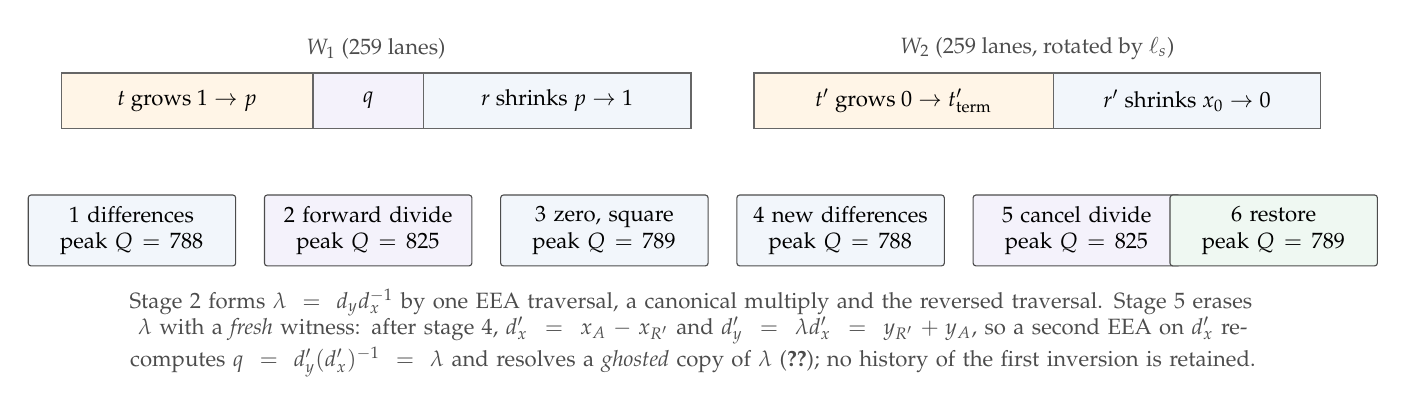
\begin{tikzpicture}[x=1cm,y=1cm,font=\footnotesize]
  % banks
  \draw[fill=lookorange,draw=black!60] (0,2.2) rectangle (3.2,2.9); \draw[fill=addviolet,draw=black!60] (3.2,2.2) rectangle (4.6,2.9); \draw[fill=gateblue,draw=black!60] (4.6,2.2) rectangle (8.0,2.9);
  \node at (1.6,2.55) {$t$ grows $1\to p$}; \node at (3.9,2.55) {$q$}; \node at (6.3,2.55) {$r$ shrinks $p\to1$};
  \node[note,anchor=south] at (4,2.95) {$W_1$ ($259$ lanes)};
  \draw[fill=lookorange,draw=black!60] (8.8,2.2) rectangle (12.6,2.9); \draw[fill=gateblue,draw=black!60] (12.6,2.2) rectangle (16.0,2.9);
  \node at (10.7,2.55) {$t'$ grows $0\to t'_{\rm term}$}; \node at (14.3,2.55) {$r'$ shrinks $x_0\to0$};
  \node[note,anchor=south] at (12.4,2.95) {$W_2$ ($259$ lanes, rotated by $\ell_s$)};
  % pipeline
  \foreach \x/\lab/\q/\col in {0.9/{1 differences}/788/gateblue,3.9/{2 forward divide}/825/addviolet,6.9/{3 zero, square}/789/gateblue,9.9/{4 new differences}/788/gateblue,12.9/{5 cancel divide}/825/addviolet,15.4/{6 restore}/789/outgreen}{
    \node[draw=black!70,fill=\col,rounded corners=1pt,text width=24mm,minimum height=9mm,align=center] at (\x,0.9) {\lab\\ peak $Q=\q$};}
  \node[note,text width=16cm] at (8,-0.4) {Stage 2 forms $\lambda=d_yd_x^{-1}$ by one EEA traversal, a canonical multiply and the reversed traversal. Stage 5 erases $\lambda$ with a \emph{fresh} witness: after stage 4, $d'_x=x_A-x_{R'}$ and $d'_y=\lambda d'_x=y_{R'}+y_A$, so a second EEA on $d'_x$ recomputes $q=d'_y(d'_x)^{-1}=\lambda$ and resolves a \emph{ghosted} copy of $\lambda$ (\cref{sec:ghost}); no history of the first inversion is retained.};
\end{tikzpicture}}
\caption{The low-$Q$ circuit \code{b6f2b0a}: the two packed banks of the register-shared EEA and the six stages with their peak widths (Supplemental Note~E, pp.\,4, 8 and 14).}
\label{fig:lowq}
\end{figure}

\subsubsection{Ghosting: measurement-based release and later recomputation}\label{sec:ghost}

The low-$Q$ route frees a whole $257$-lane field register during the reverse EEA without losing coherence. If a reversible computation has produced $\sum_x\alpha_x\ket x\ket{f(x)}_D$, measuring each lane of $D$ in the $X$ basis yields a classical string $m$ and leaves $\sum_x\alpha_x(-1)^{m\cdot f(x)}\ket x$; the lanes of $D$ are released (\cref{fig:ghost}). Later the same Boolean function is recomputed lane by lane into a fresh register ($d_y=\lambda d_x$ after $d_x$ has been restored) and $Z^{m_j}$ on each rebuilt lane contributes $(-1)^{m\cdot f(x)}$ a second time, so $(-1)^{2m\cdot f(x)}=1$ and the explicit $\ket{d_y}$ is recovered exactly. Luo et al.\ use exactly this to run their point addition on three field registers \cite{luo26}; it is valid whenever the later register holds the same function as the measured one---it is not erasure, and it does not assume $d_y$ is classical.

\begin{figure}[H]
\centering
\resizebox{0.95\textwidth}{!}{%
\begin{quantikz}[column sep=6pt,row sep=5pt,font=\small]
\lstick{$\ket x$}     & \gate[2]{\text{compute }f} & & \gate{\text{reverse EEA}} & \gate[2]{\text{recompute }f} &              & \gate[2]{\text{use}} & \\
\lstick{$\ket{0}_D$}  &                             & \gate{H}\meter{} & \setwiretype{n} & \setwiretype{q} & \gate{Z^{m}} &  & \\
\end{quantikz}}
\caption{Ghosting (Supplemental Note~E, p.\,12; \cite{luo26}). The register holding $f(x)$ is $X$-measured ($\Hmr$, outcome string $m$) and freed; the phase $(-1)^{m\cdot f(x)}$ it leaves is cancelled by $Z^{m}$ on a later, independently recomputed copy of $f(x)$.}
\label{fig:ghost}
\end{figure}

\subsection{Measurement-based uncomputation, in general}\label{sec:mbu}

Every scratch value must return to $\ket0$ with no residual phase (the reversibility and phase checks of \cref{sec:challenge}), so the question is never \emph{whether} to uncompute but \emph{how}. The textbook way---run the computation backwards---costs as many Toffolis as the computation. The alternative is the pattern already used three times above: measure the wire in the $X$ basis, which resets it but leaves a known phase $(-1)^{m\cdot f}$ depending on the random outcome $m$; then cancel that phase with gates conditioned on $m$. The whole family (census: \emph{uncompute strategy}, $22$ commits, all ``measurement uncompute'') differs only in how cheap the fix-up is \cite{ecdsafail26,ecdsafail-wiki}:
\begin{itemize}[nosep]
\item $f$ is an AND of two live wires, or any \emph{quadratic} function of live wires: the fix-up is CZ/Z gates only, $0$ Toffolis. Examples: the AND-uncompute of \cref{fig:and-adder} (\code{clear\_and}, \code{measured\_and\_clear}); the \emph{from-zero} adders (\code{5b834ba}: if an operand bit is provably $\ket0$ on entry the MAJ step leaves exactly $\mathrm{AND}(x,y)$ in it, so the UMA Toffoli becomes $\Hmr+$\code{cz\_if}); the \emph{known-output receivers} (\code{add\_known}, \code{known\_stream}: when the adder's result is already known as an affine function of live wires---a reverse pass restoring a value---each carry is rebuilt with CNOTs as $c_i=a_i\oplus b_i\oplus s_i$ and then $X$-measured; written in terms of the sum bit and the incoming carry each carry is quadratic, so the repair is Z/CZ: an adder with \emph{zero} Toffolis, valid on the subspace where the output really is known); the \emph{phase-only comparator tops} (a borrow $\MAJ(q,a,x)=qa\oplus qx\oplus ax$ needs only its phase, three CZs instead of a Toffoli).
\item $f$ is a comparison (a chunk carry-out, an overflow flag): the fix-up is a phase oracle (compute, $Z$, uncompute) under \code{push\_condition(m)}, executed on half the shots---so its \emph{executed} Toffoli cost is half its static cost, and truncating it to $k$ bits makes it approximate (\cref{sec:chunked}).
\item the opposite choice, \emph{deferred coherent uncompute} (\code{b788efc}): keep the square's chunk carries live until the inverse pass recomputes them into the held wires (exact, no conditioned compare), paying with loans of provably-zero wires.
\end{itemize}
Two things break the idiom: a control that changes after the AND was built (the CZ then applies the wrong phase), and an approximate fix-up. A systematic error shows up as \code{PHASE GARBAGE} with near certainty; a rare one adds hard inputs to the phase channel. The simulator models $\Hmr$ as: draw $m$ from the Fiat--Shamir stream, store it, $\mathrm{phase}\mathrel{\oplus}=q\wedge m$, $q\gets0$; a plain reset $R$ does the same but discards $m$, which is why freeing a dirty wire is never safe. $\Hmr$ cannot be replayed by \code{emit\_inverse}, so any backward pass containing it is written by hand.

\begin{figure}[H]
\centering
\begin{quantikz}[column sep=7pt,row sep=5pt,font=\small]
\lstick{$x$}        & \ctrl{2} & \gate[2]{\text{use }w} & \ctrl{1}   & \\
\lstick{$y$}        & \ctrl{1} &                        & \control{} & \\
\lstick{$\ket0$}    & \targ{}  &                        & \gate{H}\meter{}\wire[u][1]{c} & \setwiretype{n} \rstick{$m$}\\
\end{quantikz}
\hspace{8mm}
\begin{minipage}{0.48\textwidth}\small
compute: $w\gets x\wedge y$ (one Toffoli; four $T$ gates fault-tolerantly)\\
uncompute: $\Hmr(w\to m)$ leaves $(-1)^{m\,xy}$; apply $\mathrm{CZ}(x,y)$ iff $m=1$\\
cost of the uncompute: $0$ Toffolis, one measurement, one feed-forward bit\\
condition: $w$ must still equal $x\wedge y$ of the \emph{current} controls
\end{minipage}
\caption{Gidney's temporary logical AND with measurement-based uncomputation \cite{gidney18add}, the primitive behind the ``uncompute strategy'' family. The challenge counts the compute Toffoli and not the uncompute, which is why its $T$ is ``executed Toffolis''.}
\label{fig:and-gadget}
\end{figure}

\subsection{Post-passes, census strips, and the nonce economy}\label{sec:postpasses}

After the circuit is emitted and before the nonce tail is appended, \code{build()} runs passes over the op stream. \emph{Exact} ones: self-inverse pair cancellation (a CCX followed by the same CCX with nothing touching its operands in between), constant propagation of $\{0,1,?\}$ and affine relations (drop a CCX with a known-$0$ control, turn one with a known-$1$ control into a CX), the target-fanout identity $\mathrm{CCX}(a,b\to t);\mathrm{CX}(t\to u);\mathrm{CCX}(a,b\to t)=\mathrm{CX}(t\to u);\mathrm{CCX}(a,b\to u)$ looped to closure, the four simplifiers \code{product}, \code{affine}, \code{quadratic}, \code{truth} that re-derive Boolean support facts from the stream, and \emph{SAT-proven CCX$\to$CX rows}: an offline solver proves that a specific Toffoli's product equals a fixed XOR of other wires at that point of the stream, and the gate is replaced by a CNOT chain (the October frontier ships $105$ such rows, $102$ of them in the square). \emph{Empirical} ones: a \emph{fire census} simulates the stream on $10^8$--$10^9$ random inputs, records which Toffolis ever fired and which had an implied second control, and deletes or downgrades the rest, admitted in ascending risk until a $\lambda$ budget is spent (\code{DEAD\_KEYS}/\code{DOWNGRADE\_KEYS}, identity-keyed so that an upstream edit cannot mis-address them, after a positional strip once caused $7{,}535/9{,}024$ mismatches). As of 1~October the frontier's build ran no census strip, only the exact chain and the SAT rows \cite{ecdsafail-wiki}. Finally, \emph{verifier search}: a nonce-only change moves the score by a few Toffolis because the average is over a different sample ($-5$, $-9$, $-24$ T in three admitted commits), and every real change forces a re-hunt whose expected cost grows like $e^{\lambda}$: around $\lambda\approx8$ a hunt is minutes to hours on GPUs, at $15$--$20$ it needs a pre-filter and many GPU-hours, beyond that it is infeasible even when the Toffoli count looks better. The measured $\lambda\approx15.7$ of one tree (9.5 classical, 6.2 phase) gave one clean draw in $\approx29{,}000$ rather than the naive $e^{-15.7}\approx1/6.8$\,M, because classical and phase failures are correlated \cite{ecdsafail-wiki}.

\subsection{Making the circuit window-compatible}\label{sec:windowed}

In the challenge $A$ arrives as classical bits; in Shor's algorithm it is \emph{selected coherently} by a $w$-qubit address $J$. Supplemental Note~F adapts \code{8e9c9a2} to the interface $U_{\rm win}:\ket J\ket R\ket0_W\mapsto\ket J\ket{R+A_J}\ket0_W$: the circuit exposes $X,Y,J$ and $3\cdot2^{w}$ classical table columns ($x_j$, $y_j$, $3x_j\bmod p$, with row $0$ encoding $\mathcal O$ as zeros), conditions every payload CNOT on the runtime table bits, and \emph{replays} each lookup after use (\cref{fig:windowed}). The lookup is an XOR, $L_c:\ket j\ket z\mapsto\ket j\ket{z\oplus c_j}$, implemented by a reversible address traversal (unary iteration over the $w$ address bits with AND ancillas) that applies a classically conditioned CNOT to each payload bit whose table bit is one; applying it twice clears the payload exactly, $\ket j\ket{c_j}\mapsto\ket j\ket0$, and the traversal's routing ANDs are removed by measurement with phase correction. Stage 3 uses a $K=2$ QROAM \cite{lks18}: with $j=2h+\ell$ the high-address traversal loads two adjacent rows into banks $B_0,B_1$ and $\ell$-controlled swaps select the requested one. The identity row is handled by a coherent predicate $b=[J\ne0]$ that controls the square-subtract of stage 4 and the negation of stage 6, so $R+\mathcal O=R$ without measuring $J$. Cost: $Q=1{,}162$ ($+11$, because the payload banks are cleared before the dialog-GCD peak), $T=1{,}683{,}828$ ($+29.6\%$; the three traversal pairs cost $328{,}180$ executed Toffolis), serialised operations $25.21\times$ more (table-payload CNOTs), error rate $0.1950\%$ against the baseline's $0.1920\%$ on a shared $100{,}000$-input corpus---statistically indistinguishable \cite{ecdsafail-supp}.

\begin{figure}[H]
\centering
\resizebox{\textwidth}{!}{%
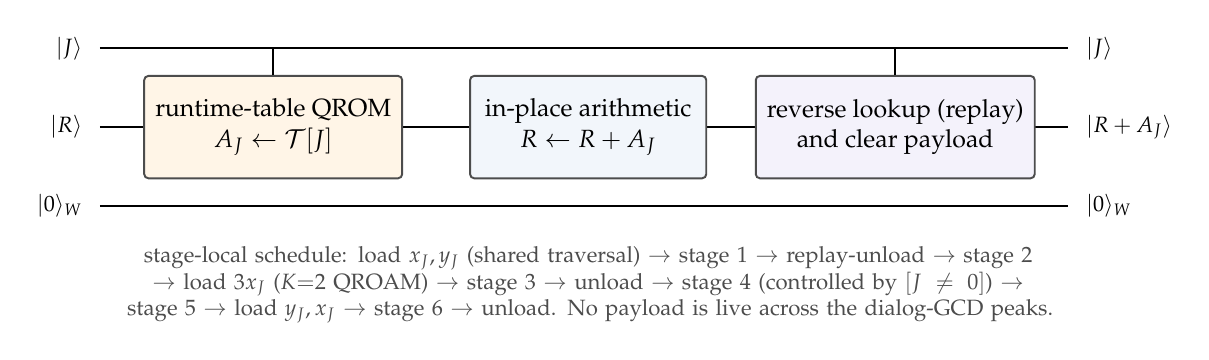
\begin{tikzpicture}[x=1cm,y=1cm,font=\footnotesize]
  \node[anchor=east] at (0,2.2) {$\ket J$}; \node[anchor=east] at (0,1.2) {$\ket R$}; \node[anchor=east] at (0,0.2) {$\ket0_W$};
  \draw[wire] (0.1,2.2)--(12.4,2.2); \draw[wire] (0.1,1.2)--(12.4,1.2); \draw[wire] (0.1,0.2)--(12.4,0.2);
  \node[blko,minimum width=26mm,minimum height=13mm] (l) at (2.3,1.2) {runtime-table QROM\\$A_J\gets\mathcal T[J]$};
  \node[blk,minimum width=30mm,minimum height=13mm] (a) at (6.3,1.2) {in-place arithmetic\\$R\gets R+A_J$};
  \node[blkv,minimum width=28mm,minimum height=13mm] (u) at (10.2,1.2) {reverse lookup (replay)\\and clear payload};
  \draw[wire] (2.3,2.2)--(l.north); \draw[wire] (10.2,2.2)--(u.north);
  \node[anchor=west] at (12.5,2.2) {$\ket J$}; \node[anchor=west] at (12.5,1.2) {$\ket{R+A_J}$}; \node[anchor=west] at (12.5,0.2) {$\ket0_W$};
  \node[note,text width=12.4cm] at (6.3,-0.8) {stage-local schedule: load $x_J,y_J$ (shared traversal) $\to$ stage 1 $\to$ replay-unload $\to$ stage 2 $\to$ load $3x_J$ ($K{=}2$ QROAM) $\to$ stage 3 $\to$ unload $\to$ stage 4 (controlled by $[J\neq0]$) $\to$ stage 5 $\to$ load $y_J,x_J$ $\to$ stage 6 $\to$ unload. No payload is live across the dialog-GCD peaks.};
\end{tikzpicture}}
\caption{The runtime-table window interface of the window-compatible \code{8e9c9a2} (Supplemental Note~F, Figs.\,1--2).}
\label{fig:windowed}
\end{figure}

\section{The Pareto frontier}\label{sec:pareto}

\subsection{Three constructions, and which one is a frontier}

Supplemental Note~A is careful to keep three objects apart \cite{ecdsafail-supp}. The \emph{product-score incumbent sequence} is the chronological list of promoted submissions, each of which lowered $\QT$ when it landed; it is what the leaderboard shows and what \cref{fig:trajectory} plots. The \emph{low-width track} is a mechanism-oriented selection of validator-clean circuits below the product-efficient regime (q980, q988, q952, q1019, q948, q828, q826, q825 in ledger order). The \emph{admitted $(Q,T)$ Pareto set} is the only one of the three that is a frontier in the multi-objective sense,
\begin{equation}\label{eq:pareto}
\mathcal P(\mathcal A)=\{c\in\mathcal A:\ \nexists\,d\in\mathcal A\ \text{with } Q(d)\le Q(c),\ T(d)\le T(c),\ \text{one inequality strict}\},
\end{equation}
over the set $\mathcal A$ of \emph{admitted} rows: promoted ones, plus rejected ones (``rejected'' is the CLI's word for a valid run that did not beat the incumbent) that carry public evidence of a complete $9{,}024$-instance clean run. At the 26~July cutoff $\mathcal P$ had eight points, six of them rejected low-$Q$ rows that a winner-only leaderboard would have discarded (\cref{tab:pareto}).

\begin{table}[H]
\centering\small
\begin{tabular}{@{}lrrlp{5.6cm}@{}}
\toprule
submission & $Q$ & $T$ & status & interpretation\\
\midrule
\multicolumn{5}{@{}l}{\emph{Admitted Pareto set at the data cutoff, 26 July 2026 (Table~2 of the paper)}}\\
\code{b6f2b0a} & 825 & 489,161,900 & admitted & lowest admitted width (register-shared EEA)\\
\code{f1d8707} & 826 & 479,337,428 & admitted & one qubit coincides with $9{,}824{,}472$ fewer Toffolis\\
\code{39a9b5f} & 828 & 448,102,916 & admitted & two more qubits, $31{,}234{,}512$ fewer ($\approx15.6$\,M per qubit)\\
\code{a3b0148} & 948 & 54,781,961 & admitted & exit from the hard-$Q$ metadata cliff\\
\code{4352cfb} & 980 & 28,847,321 & admitted & lowest admitted $T$ below $1{,}000$ qubits\\
\code{1c0e0e9} & 1,133 & 1,460,511 & admitted & bridge toward the product-efficient regime\\
\code{8e9c9a2} & 1,151 & 1,299,453 & promoted & $\QT$ incumbent, $1{,}495{,}670{,}403$\\
\code{a536a48} & 1,158 & 1,292,651 & promoted & lowest-$T$ promoted point\\
\midrule
\multicolumn{5}{@{}l}{\emph{Non-dominated rows of the 7 October 2026 snapshot, promoted or rejected with API metrics \cite{ecdsafail-wiki}}}\\
\code{10177cd} & 792 & 656,602,578 & rejected & lowest width on the snapshot\\
\code{87cffbd} & 794 & 415,821,960 & rejected & \\
\code{8d26593} & 795 & 300,862,444 & rejected & \\
\code{c60617f} & 807 & 276,427,457 & rejected & \\
\code{5c4ec19} & 822 & 250,088,365 & rejected & \\
\code{3170f7b} & 823 & 154,247,477 & rejected & \\
\code{05f08d8} & 833 & 61,654,186 & rejected & \\
\code{48d934d} & 838 & 22,019,787 & rejected & \\
\code{a9d89c2} & 973 & 11,844,334 & rejected & \\
\code{9d4282b} & 998 & 10,438,839 & rejected & \\
\code{4188053} & 1,011 & 9,329,693 & rejected & \\
\code{57aa8ae} & 1,072 & 2,791,974 & rejected & \\
\code{c1c0da9} & 1,112 & 1,739,356 & rejected & \\
\code{dd3621d} & 1,145 & 1,132,785 & rejected & \\
\code{17250b2} & 1,164 & 970,983 & rejected & \\
\code{b72ce1a} & 1,170 & 946,553 & promoted & Skywalk, 6 Oct\\
\code{ee41004} & 1,174 & 943,826 & promoted & Skywalk, 3 Oct\\
\code{c039e59} & 1,243 & 802,520 & promoted & Leapfrog, 7 Oct\\
\code{a02c716} & 1,244 & 797,905 & promoted & Leapfrog, 7 Oct: $\QT=992{,}593{,}820$\\
\bottomrule
\end{tabular}
\caption{The admitted Pareto set of the paper and the non-dominated set of the latest public snapshot. The post-cutoff ``rejected'' rows passed the evaluator ($0/0/0$ on their own island) but did not improve the scalar score; the paper's stricter curation (a public note with a full clean run) was not re-applied here, so the lower block is the API-reported frontier, not a re-audited one. Several intermediate promoted rows ($1{,}171$--$1{,}173$ qubits) are omitted for brevity.}
\label{tab:pareto}
\end{table}

\begin{figure}[H]
\centering
\begin{tikzpicture}
\begin{loglogaxis}[width=0.93\textwidth,height=0.6\textwidth,
  xlabel={peak logical qubits $Q$}, ylabel={average executed Toffolis $T$ per point addition},
  xmin=700,xmax=3200,ymin=5e5,ymax=2e9, grid=both, grid style={black!10},
  legend style={font=\scriptsize,at={(0.98,0.98)},anchor=north east,cells={anchor=west}}, legend columns=1,
  tick label style={font=\footnotesize}, label style={font=\small},
  log ticks with fixed point, xtick={800,1000,1500,2000,3000}, xticklabels={800,1000,1500,2000,3000}]
\addplot[only marks,mark=*,mark size=0.9pt,color=black!28] table[x=q,y=t] {data/rejected_qt.dat};
\addlegendentry{rejected, valid run (7 Oct snapshot)}
\addplot[only marks,mark=*,mark size=1.0pt,color=boxblue!70] table[x=q,y=t] {data/promoted_qt.dat};
\addlegendentry{promoted (580, 30 May--7 Oct)}
\addplot[const plot mark right,thick,color=boxred] table[x=q,y=t] {data/frontier_oct7_all.dat};
\addlegendentry{non-dominated set, 7 Oct (all valid rows)}
\addplot[only marks,mark=square*,mark size=2.2pt,color=boxgreen] coordinates {(825,489161900) (826,479337428) (828,448102916) (948,54781961) (980,28847321) (1133,1460511) (1151,1299453) (1158,1292651)};
\addlegendentry{admitted Pareto set, 26 Jul (paper)}
\addplot[only marks,mark=diamond*,mark size=3pt,color=orange!80!black] coordinates {(1175,2700000) (1425,2100000)};
\addlegendentry{Google/Babbush et al.\ (upper bounds, incl.\ lookups)}
\addplot[only marks,mark=triangle*,mark size=3pt,color=violet] coordinates {(1192,2391000) (1446,1863000)};
\addlegendentry{Schrottenloher space / gate ($2^{21.19}$, $2^{20.83}$)}
\addplot[only marks,mark=pentagon*,mark size=3pt,color=teal] coordinates {(1169,2090000) (1050,32300000)};
\addlegendentry{TrailMix jump-lowqubit / shrunken-PZ}
\addplot[only marks,mark=o,mark size=3pt,thick,color=magenta!70!black] coordinates {(835,70290000)};
\addlegendentry{Luo et al.\ (three field registers)}
\addplot[only marks,mark=otimes*,mark size=3pt,color=cyan!60!black] coordinates {(1457,1392608)};
\addlegendentry{IonQ, incl.\ $3\cdot2^{16}$ lookups}
\addplot[only marks,mark=x,mark size=3.5pt,very thick,color=boxred!80!black] coordinates {(1162,1683828)};
\addlegendentry{ECDSA.fail windowed variant (lookups included)}
\addplot[only marks,mark=star,mark size=3.5pt,very thick,color=black] coordinates {(1457,1310693) (1246,2821091) (851,85204396) (1107,86033905) (2233,1426965) (1845,1432285) (1798,8346972)};
\addlegendentry{built in \texttt{shor/} (windowed, incl.\ lookups; see \cref{sec:shor-impl})}
\end{loglogaxis}
\end{tikzpicture}
\caption{The $(Q,T)$ plane. Grey and blue dots are every valid run on the 7~October snapshot ($459$ rejected, $580$ promoted); the red staircase is their non-dominated set; green squares are the paper's admitted Pareto set at the cutoff. The external points are plotted where the sources put them, but they are \emph{not} measured under one accounting rule: Google's two points are upper bounds attested by a zero-knowledge proof for a circuit that includes coherent lookups; Schrottenloher's, TrailMix's, IonQ's and the \code{shor/} points are windowed additions that include their table lookups (\cref{sec:windowed}); the \ecdsafail{} points are for a classical addend and executed Toffolis on the challenge distribution. The paper's own external table carries the same caveat \cite{ecdsafail26}.}
\label{fig:pareto}
\end{figure}

\begin{figure}[H]
\centering
\begin{tikzpicture}
\begin{semilogyaxis}[width=0.93\textwidth,height=0.5\textwidth,
  xlabel={days since 29 May 2026}, ylabel={promoted score $\QT$},
  xmin=0,xmax=135,ymin=8e8,ymax=1.3e10, grid=both, grid style={black!10},
  tick label style={font=\footnotesize}, label style={font=\small}]
\addplot[const plot,thick,color=boxblue] table[x=days,y=score] {data/incumbents.dat};
\foreach \d/\lab in {4/{dialog GCD},21/{TrailMix Jump-2},84/{ping-pong},123/{Skywalk},131/{Leapfrog}} {
  \addplot[dashed,color=black!50] coordinates {(\d,8e8) (\d,1.3e10)};
}
\node[font=\scriptsize,rotate=90,anchor=south] at (axis cs:4,2.5e9) {dialog GCD};
\node[font=\scriptsize,rotate=90,anchor=south] at (axis cs:21,2.5e9) {TrailMix Jump-2};
\node[font=\scriptsize,rotate=90,anchor=south] at (axis cs:84,3e9) {ping-pong};
\node[font=\scriptsize,rotate=90,anchor=south] at (axis cs:123,3e9) {Skywalk};
\node[font=\scriptsize,rotate=90,anchor=south] at (axis cs:131,3e9) {Leapfrog};
\node[font=\scriptsize,anchor=west] at (axis cs:2,1.05e10) {Kaliski baseline $2{,}715\times3{,}960{,}753$};
\addplot[only marks,mark=*,mark size=1.8pt,color=boxred] coordinates {(58.39,1495670403)};
\node[font=\scriptsize,anchor=north west] at (axis cs:59,1.55e9) {\code{8e9c9a2} (26 Jul)};
\addplot[only marks,mark=*,mark size=1.8pt,color=boxred] coordinates {(131.4,992593820)};
\node[font=\scriptsize,anchor=north east] at (axis cs:130,1.0e9) {\code{a02c716} (7 Oct)};
\end{semilogyaxis}
\end{tikzpicture}
\caption{The product-score incumbent sequence: all $580$ promoted submissions on the 7~October snapshot, with the five changes of inversion architecture marked. From $10.75\times10^9$ to $0.99\times10^9$ in $131$ days; the paper's three eras (I: joint peak owners, to $5.69$\,B at \code{375fdff}; II: hosted and decoded history, to $1.83$\,B at \code{4b7d727}; III: last-consumer proofs, to $1.57$\,B at \code{71f5115}) all lie inside the first two architectures \cite{ecdsafail-supp}.}
\label{fig:trajectory}
\end{figure}

\subsection{Reading the frontier}

\paragraph{The secants are not marginal costs.} Moving from $826$ to $828$ qubits coincides with $31.2$\,M fewer Toffolis, about $15.6$\,M per qubit; from $980$ to $1{,}133$ with more than $27$\,M fewer; from $1{,}133$ to $1{,}151$ with only $161{,}058$ fewer, and from $1{,}151$ to $1{,}158$ with $6{,}802$. These are descriptive secants between \emph{different circuit families}, not derivatives of one design; what they evidence is a steep ``hard-$Q$'' transition among the observed routes, a cliff below $\approx950$ qubits where resident arithmetic state has been replaced by metadata and recomputation and the Toffoli count rises by orders of magnitude \cite{ecdsafail-supp}. The fixed-budget slices are discontinuous for the same reason: no admitted circuit between $981$ and $1{,}050$ qubits improved on the $980$-qubit row's count.

\paragraph{What the frontier is relative to.} The baseline of the challenge was $2{,}715\times3{,}960{,}753=10.75$\,B (with the $9{,}000$-pair \code{DUMMY\_TOFFOLIS} padding; $3{,}942{,}753$ unpadded). The cutoff incumbent \code{8e9c9a2} is $86.1\%$ lower ($7.19\times$); its $Q$ fell $57.6\%$ and its $T$ $67.2\%$; the product tip ($1{,}151$) and the Toffoli tip ($1{,}158$, \code{a536a48}) are different rows. The 7~October incumbent \code{a02c716} is $90.8\%$ below the baseline; it spent $93$ qubits to buy $502$k Toffolis relative to \code{8e9c9a2}. Google's attested points are $3.17$\,B and $2.99$\,B retry-adjusted (their reported circuits were treated as zero-error); the paper's claim is that the challenge reached ``more than 50\% below'' them \emph{under its own accounting}, which excludes the coherent lookups that Google's circuits include (\cref{sec:windowed}: adding them costs $+11$ qubits and $+29.6\%$ Toffolis) \cite{ecdsafail26}.

\paragraph{Retry-adjusted scores.} Because frontier circuits are approximate, the paper also plots $\QT/\hat p$ with $\hat p$ the success rate on a common $50{,}000$-input corpus and, for a full attack with $28$ additions, $28\,Q'T'/(1-28e)$ with $Q'=Q+16$, $T'=T+3\cdot2^{16}$, $e=1-\hat p$; $\hat p$ stays near $1$ on the point-addition axis (the $0.192\%$ failure of \code{8e9c9a2} would cost $\approx5.3\%$ additional expected work under an independently re-runnable success model), but some nominal improvements shrink or reverse once the $28\times$ amplification is applied, and the union bound is only a plug-in proxy: $\hat p$ measures classical-output agreement, not coherent circuit success, and silent errors inside Shor's algorithm accumulate coherently across additions \cite{ecdsafail26,ecdsafail-supp}.

\begin{table}[H]
\centering\small
\begin{tabular}{@{}p{5.4cm}rrp{5.8cm}@{}}
\toprule
artifact & $Q$ & Toffolis & accounting\\
\midrule
Google/Babbush low-$Q$ \cite{babbush26} & 1,175 & $2.7$\,M & disclosed upper bound (ZK proof); lookups included\\
Google/Babbush low-gate \cite{babbush26} & 1,425 & $2.1$\,M & same package\\
Schrottenloher space-optimised \cite{schrottenloher26} & 1,192 & $2^{21.19}$ & reproducible architecture, windowed, plus $16$ window qubits\\
Schrottenloher gate-optimised \cite{schrottenloher26} & 1,446 & $2^{20.83}$ & \\
TrailMix \code{jump-lowqubit} \cite{ecdsafail26} & 1,169 & $2.09$\,M & open implementation prior\\
TrailMix \code{shrunken-PZ} \cite{ecdsafail26} & 1,050 & $32.3$\,M & architectural prior for the low-$Q$ track\\
Luo et al.\ \cite{luo26} & 835 & $70.29$\,M & $3n+6\lfloor\log_2n\rfloor+19$ qubits\\
IonQ/H\"aner et al.\ \cite{haener26} & 1,457 & $1.196$\,M $+3\cdot2^{16}$ & windowed, signed-window ready; $28$ additions $\Rightarrow39.0$\,M\\
\ecdsafail{} \code{8e9c9a2} & 1,151 & $1{,}299{,}453$ & classical addend, executed Toffolis\\
\ecdsafail{} windowed \code{8e9c9a2} (Note F) & 1,162 & $1{,}683{,}828$ & coherent lookups included\\
\ecdsafail{} \code{a02c716} (7 Oct) & 1,244 & $797{,}905$ & classical addend\\
\ecdsafail{} \code{b6f2b0a} / \code{10177cd} & 825 / 792 & $489$\,M / $657$\,M & extreme-width evidence\\
\code{shor/}: IonQ cells, signed windows, SELECT-SWAP & 1,457 & $1{,}310{,}693$ & windowed, executed; $37.1$\,M for $28$ additions\\
\code{shor/}: dialog on the space cells & 1,246 & $2{,}821{,}091$ & windowed\\
\code{shor/}: three field registers (Luo) & 851 & $85{,}204{,}396$ & windowed; $2.39$\,G for the attack\\
\bottomrule
\end{tabular}
\caption{Neighbouring public operating points for one secp256k1 point addition, under heterogeneous accounting rules (after Table~3 of \cite{ecdsafail26}, extended). ``Reported count'' is not a uniform metric across rows.}
\label{tab:external}
\end{table}

\section{The \code{shor/} implementation against the \ecdsafail{} catalogue}\label{sec:shor-impl}

The Qiskit package in \code{shor/shor\_qiskit/} ($44$ modules, $\approx16{,}700$ lines, plus $\approx4{,}400$ lines of benchmarks in \code{bench/}) builds the same object the challenge scores---one windowed secp256k1 point addition---from exhaustively tested toy-size primitives, and counts its $256$-bit instantiation hierarchically (\code{hier.tracing()}: build each sub-circuit once per \emph{shape}, append it as an opaque gate carrying its counts; at toy size the hierarchical count equals the flat one on every field and the tree exports to Qualtran bloqs whose \code{QECGatesCost} agrees). This section records which of the \ecdsafail{} levers it already contains, what it measures for them, and what it does not have. The numbers are the package's own, from \code{bench/*.json} and \code{shor-complete.tex} Part~VII.

\subsection{Coverage}

\begin{table}[H]
\centering\footnotesize
\begin{tabular}{@{}p{4.0cm}p{5.2cm}p{6.3cm}@{}}
\toprule
\ecdsafail{} lever (section) & in \code{shor/} & measured (\code{secp256k1}, $w=16$)\\
\midrule
Kaliski almost-inverse, HJNRS form (\cref{sec:inversions}) & \code{ec\_kaliski}, \code{ec\_kaliski\_opt} (unconditional rounds, postponed reduction, Montgomery form) & $29\%$ fewer Toffolis and $41\%$ less depth than HJNRS at $n=12$\\
dialog GCD, record/replay (\cref{sec:dialog}) & \code{ec\_eea} (as printed), \code{ec\_gcd.Dialog} (fused 77-bit compare, width schedule, PM cells) & in-place multiply $1{,}955{,}276\to865{,}588$ Toffolis\\
IonQ's conditionally-inverted walk, Fig.\,1 record packing ($3$ pairs in $5$ qubits) & \code{ec\_gcd.CondInv}, \code{fig1\_compress} & $720{,}565$ per in-place multiply; record $669$ qubits\\
Jump-2 (\cref{sec:jump2}) & \code{ec\_gcd.Jump2}, \code{Jump2Packed} ($261$ steps) & $1{,}161{,}099$ per multiply from this package's generic cells (no fused cells, no base-5 codec)\\
ping-pong (\cref{sec:pingpong}) & \code{ec\_gcd.PingPong} ($704$ rounds) & $917{,}565$ per multiply; walk $257$/round, replay $785$/step; $2{,}117{,}534$ per addition on $2{,}155$ qubits\\
register-shared EEA, three field registers (\cref{sec:regshare}) & \code{ec\_luo}, \code{ec\_luo3} (ghosting via \code{ec\_mbu.vent}/\code{zfix}) & division $835$ qubits / $42{,}103{,}470$ T; windowed addition $851$ / $85{,}204{,}396$; attack $2.386\times10^9$\\
Gidney classical--quantum constant adder & \code{ec\_cqadd} & $2.98n$ (dirty) / $3.96n$ (3 clean) Toffolis; mod add $11.0n$, doubling $6.0n$ (Luo's $11n$, $6n$)\\
temporary-AND adder, measured uncompute (\cref{sec:adders,sec:mbu}) & \code{ec\_gates.and\_/and\_dg}, \code{ec\_adders} & $2.50\times$ fewer $T$ over an inversion; CDKM vs Gidney $2n$ vs $n-1$\\
pseudo-Mersenne folds, truncated compares (\cref{sec:fold,sec:truncation}) & \code{ec\_approx} (Alg.\,5--11 of \cite{schrottenloher26}), \code{PMPhase} (IonQ's phase-approximate adder, $\kappa=65$, $\delta=32$, 37 careful steps) & cell $712\to352$ Toffolis ($336$ executed); failure rates measured at toy primes\\
dedicated squarer with fold (stage 4) & \code{ec\_square} (IonQ's signed-row squarer) & $1{,}050{,}623\to79{,}160$ Toffolis per square-subtract\\
QROM lookups, MBU unlookup, merged phase repair, SELECT-SWAP & \code{ec\_window}, \code{ec\_mbu}, \code{select\_swap\_lookup} & $1{,}310{,}700\to197{,}364$ per addition; SELECT-SWAP on the $3x$ load $-16{,}128$ at no qubit cost\\
signed windows & \code{ec\_signedwin} & $2^{15}$-entry tables, $-2.7$\,M over $28$ additions\\
exact peepholes, fire census (\cref{sec:postpasses}) & \code{ec\_opt.peephole}, \code{ec\_opt.census}/\code{strip\_unfired} & census at $q=61$: exact when it covers all inputs ($1{,}680\to991$); $2.8\%$ of fresh inputs wrong at $300$ samples\\
lean (space) cells, register sharing beside the walk & \code{ec\_space} (\code{PMSpace}), \code{CondInv(share=True)} & $1{,}246$ qubits at $2{,}821{,}091$ T; $1{,}457$ at $1{,}310{,}693$ executed\\
carry-lookahead adders & \code{ec\_cla} & $7\times$ Toffolis for $\log n$ depth; addition depth $1{,}503{,}533\to394{,}281$\\
physical model (\cref{sec:physical}) & \code{physical.py} (Gidney-2025 surface-code model) & reproduces $897{,}864$ qubits / $4.96$ days for RSA-2048\\
\bottomrule
\end{tabular}
\caption{What the package already implements of the \ecdsafail{} catalogue, with its own measurements (\code{bench/ec\_project\_256.json}, \code{ec\_toffoli\_256.json}, \code{ec\_space\_256.json}, \code{ec\_luo3\_256.json}, \code{ec\_catalogue.json}, \code{estimates.json}).}
\label{tab:coverage}
\end{table}

Three of its results sit directly on the plane of \cref{fig:pareto}: the IonQ-style addition with signed windows and SELECT-SWAP on the $3x$ lookup, $1{,}457$ qubits and $1{,}310{,}693$ executed Toffolis ($5.9\%$ below IonQ's $1{,}392{,}608$ at IonQ's own width), the space variant at $1{,}246$ qubits, and the three-register Luo circuit at $851$ qubits---the top of \ecdsafail{}'s published low-$Q$ range. The package also makes a point that the challenge metric hides: every ripple-based construction has a Toffoli \emph{depth} of $0.8$--$0.95\times$ its Toffoli count, so the fast machine of \cref{sec:physical} is throughput-bound, not reaction-bound, until carry-lookahead adders (\code{ec\_cla}, $\approx7\times$ the Toffolis for $\log n$ depth) are used, after which the unary-iteration lookups set a floor of $3\cdot2^{16}=196{,}608$ steps per addition.

\subsection{What the package does not have, and what it would take}

\begin{enumerate}[leftmargin=*]
\item \textbf{The post-August walks.} \code{ec\_gcd} has Kaliski, the dialog, CondInv, Jump-2 and ping-pong as backends on one \code{backend.mul(m,x,y,q)} interface, which is exactly the right place for \emph{Skywalk} (\cref{sec:skywalk}) and \emph{Leapfrog} (\cref{sec:leapfrog}). Leapfrog is the natural next backend: its rails are two odd two's-complement registers, its tick is three add-halves and a barrel, its letter is five raw qubits (no codec), and its payload cell is ping-pong's \code{replay\_add\_halve} run at the proxy round of the rail width---all of which the package has or can compose from \code{PMPhase}. The parts that need new code are the choice rule (\emph{sign2} plus the $K$-bit window compare), the barrel ($\mathrm{rot4}$ from three controlled reflections, and the payload's $\times2^{-e}\bmod p$ via $P-m(f-1)$), and the width-envelope fit. The package's own round-budget caveat applies: it found ping-pong's $704$ rounds not to be a worst case ($n=16$ needs $3.9n$ exhaustively), so a Leapfrog port should re-measure the parking depth rather than inherit $139$.
\item \textbf{The base-5 codec and the live-width schedule of stage 2.} \code{Jump2Packed} packs symbols but not as base-5 digits; the $609$-versus-$783$ tape, and the Note-D objective of making the shrinking $2w_i$ absorb the growing $|\tau_i|$ (\cref{eq:livewidth}), are what take a Jump-2 circuit from this package's $2{,}217$ qubits to the challenge's $1{,}151$. The package's \code{CondInv(share=True)} already does the equivalent for IonQ's walk (the record grows into the lanes the width schedule frees); the same mechanism applied to \code{Jump2Packed} with the codec is a contained change.
\item \textbf{Fused replay cells.} The challenge's replay step costs $\approx785$ Toffolis in the package's generic cells but far less in the fused \code{signed\_mod\_add\_pm\_halve\_fused}/\code{replay\_add\_halve} cell (chunked add with measured boundary carries, selected fold by $\{-f,0,+f,+2f\}$, measured flag). The package's \code{PMPhase.signadd} is the same idea for IonQ's adder; the remaining gap is the fused halving-with-fold and the per-round chunk/flag/fold \emph{shapes}.
\item \textbf{$\lambda$-priced truncation and nonce hunting.} The package measures failure rates of each approximate cell at toy primes and composes them; it does not do what every frontier submission does, which is to fit width schedules against a $\lambda$ budget on the actual $256$-bit distribution and to hunt an island. That machinery is not needed for an honest resource estimate (the package's circuits are either exact or carry a measured rate), but it is needed to \emph{reproduce} a frontier score, because the frontier scores are island-conditioned. A classical pre-filter replaying the walk's failure predicate (as \code{dialog\_gcd\_classical\_filter.rs} and the CUDA kernels do) would be the first step.
\item \textbf{Zero-Toffoli known-output receivers and the exact simplifier chain.} \code{add\_known} and \code{known\_stream} (\cref{sec:mbu}) and the \code{product}, \code{affine}, \code{quadratic}, \code{truth} passes are generic and would apply to the package's reverse passes; the SAT-proven CCX$\to$CX rows are stream-specific and not worth porting.
\item \textbf{Window compatibility is already there.} Because the package builds the windowed addition with coherent lookups (unlike the challenge interface), its numbers are the ``full-attack'' numbers directly; the conversion of \cref{eq:full-attack} is not needed for them. The identity row and the $R\in\{\pm A\}$ exceptions are handled as in Note~F, with signed windows removing $\mathcal O$ from the tables altogether.
\item \textbf{Physical model.} \code{physical.py} is a surface-code model; \cref{sec:physical} adds the trapped-ion (IonQ Q102), gross-code (IBM) and neutral-atom data points and explains why they are not modelled the same way.
\end{enumerate}

\begin{keybox}[title={The one-line comparison}]
On the challenge's own axis the package's best windowed addition is $1{,}457\times1{,}310{,}693=1.91$\,B---above \ecdsafail{}'s $1.50$\,B (classical addend) and $1.96$\,B (windowed) and above IonQ's $2.03$\,B---while being exact wherever it is not explicitly approximate, and verified end to end at toy sizes. The frontier's remaining advantage is almost entirely in the walk (Leapfrog's $139$ fat ticks against $401$ CondInv rounds) and in the fused replay cell; the frontier's disadvantage is that its best numbers are island-conditioned.
\end{keybox}


\clearpage
\part{Fault tolerance: from logical to physical qubits}
\section{Why error correction, and what it costs}\label{sec:qec-why}

\subsection{Noise, and the discretisation of errors}

A circuit of $N$ logical qubits and $G$ gates run directly on physical hardware fails with probability $\approx Gp$, where $p$ is the error per operation. The circuits of Part~I have $G\approx4\times10^7$ Toffolis---each itself several two-qubit gates---on $\approx1{,}200$ qubits, while the best physical two-qubit gates in 2026 sit at $p\sim10^{-3}$ (superconducting) to $10^{-4}$ (trapped ions) \cite{willow25,walkingcat26}. The gap of five to ten orders of magnitude is closed by quantum error correction, whose two founding facts are:

\begin{enumerate}[leftmargin=*]
\item \textbf{Errors can be discretised.} Any single-qubit noise process is a linear combination of $I,X,Y,Z$ (its Kraus operators expand in the Pauli basis), so a code that corrects $X$, $Y$ and $Z$ on any one qubit corrects \emph{every} single-qubit error, and the measurement of the syndrome projects a continuous error onto one of the discrete Pauli cases. Formally, a set of errors $\{E_a\}$ is correctable by a code with projector $\Pi$ iff the \emph{Knill--Laflamme conditions} hold \cite{knill-laflamme97}:
\begin{equation}\label{eq:KL}
\Pi\,E_a^\dagger E_b\,\Pi=c_{ab}\,\Pi\qquad\text{for all }a,b ,
\end{equation}
i.e.\ no error maps a codeword onto another codeword, and different errors are either distinguishable or act identically on the code (\emph{degeneracy}).
\item \textbf{Fault tolerance is possible below a threshold.} If every component fails with probability below some $p_{\rm th}$, then arbitrarily long quantum computations can be carried out with arbitrarily small logical error at a cost that is polylogarithmic in the circuit size (the threshold theorem \cite{aharonov-benor08,knill05}). The proof concatenates a distance-$3$ code with itself $\ell$ times: one level turns $p$ into $cp^2$ (two faults are needed to fail), so $\ell$ levels give $p_\ell=(cp)^{2^\ell}/c$, which is $\le\varepsilon$ once $\ell=O(\log\log(1/\varepsilon))$, at a size overhead of $n^\ell=\mathrm{polylog}(1/\varepsilon)$.
\end{enumerate}

In practice the overhead is dominated not by the asymptotics but by the constants of the code family, so the right question is: \emph{for a given physical error rate $p$ and a target logical error $\varepsilon$ per gate, how many physical qubits does a logical qubit cost, and how many does a logical gate cost?} The answer for the surface code is set by its threshold $p_{\rm th}\approx1\%$ and the empirical law
\begin{equation}\label{eq:plaw}
p_L(d)\approx A\Big(\frac{p}{p_{\rm th}}\Big)^{(d+1)/2},\qquad A\approx0.1,
\end{equation}
per code-distance-$d$ patch per round of syndrome measurement \cite{fowler12,fowler-gidney18}, so that each step $d\to d+2$ suppresses the logical error by $\Lambda=p_{\rm th}/p$ (Google measured $\Lambda=2.14\pm0.02$ on Willow at its physical noise \cite{willow25}; \cref{fig:threshold} shows $\Lambda\approx10$ at $p=10^{-3}$ for the circuit-level depolarising model simulated here). A distance-$d$ patch costs $2d^2-1$ physical qubits ($d^2$ data, $d^2-1$ measurement), so a target of $\varepsilon=10^{-15}$ per patch per round at $p=10^{-3}$ needs $d\approx25$ and $\approx1{,}250$ physical qubits per logical qubit before any routing space---the origin of the ``$\sim10^3$ physical qubits per logical qubit'' rule of thumb and of the million-qubit estimates of \cref{sec:physical}.

\subsection{The stabiliser formalism}\label{sec:stabiliser}

Let $\mathcal P_n$ be the Pauli group on $n$ qubits (tensor products of $I,X,Y,Z$ with phases $\pm1,\pm i$). A \emph{stabiliser code} is defined by an abelian subgroup $\mathcal S=\langle S_1,\dots,S_{n-k}\rangle\subset\mathcal P_n$ with $-I\notin\mathcal S$; its code space is the joint $+1$ eigenspace $\mathcal C=\{\ket\psi:\ S\ket\psi=\ket\psi\ \forall S\in\mathcal S\}$, of dimension $2^k$ when the $n-k$ generators are independent \cite{gottesman97,crss98}. Three facts carry the whole subject:
\begin{itemize}[leftmargin=*]
\item \textbf{Detection.} For a Pauli error $E$, either $E$ commutes with every generator or it anticommutes with some of them; measuring the generators returns the \emph{syndrome} $s\in\{0,1\}^{n-k}$, $s_i=1$ iff $E$ anticommutes with $S_i$, without disturbing the encoded state, because the measurement of $S_i$ projects onto its $\pm1$ eigenspaces and the code state is already an eigenstate.
\item \textbf{Logical operators.} The \emph{normaliser} $N(\mathcal S)$ (Paulis commuting with all of $\mathcal S$) acts on $\mathcal C$; $N(\mathcal S)/\mathcal S$ is the $2k$-generated group of logical Paulis $\bar X_j,\bar Z_j$. An undetectable error is an element of $N(\mathcal S)$; it is harmless iff it lies in $\mathcal S$. The \emph{distance} is $d=\min\{\wt(E):E\in N(\mathcal S)\setminus\mathcal S\}$, and the code corrects all errors of weight $\le t=\lfloor(d-1)/2\rfloor$ (\cref{eq:KL}: for $\wt(E_a^\dagger E_b)<d$ the product is either in $\mathcal S$ or detectable).
\item \textbf{Binary representation.} Writing a Pauli as a $2n$-bit vector $(x|z)$ (ignoring phase), products become sums mod $2$ and commutation becomes the symplectic form $x\cdot z'+z\cdot x'\bmod2$; the generators form an $(n-k)\times2n$ \emph{check matrix} $H=[H_X|H_Z]$ with $H_XH_Z^{\mathsf T}+H_ZH_X^{\mathsf T}=0$, and the syndrome of $E=(x|z)$ is $s=H_Xz+H_Zx$. Decoding, encoding and the bounds of \cref{sec:bounds} are all linear algebra over $\F_2$ on $H$.
\end{itemize}
A \emph{CSS code} \cite{calderbank-shor96,steane96} has generators that are purely $X$-type or purely $Z$-type, $H=\big[\begin{smallmatrix}H_X&0\\0&H_Z\end{smallmatrix}\big]$ with $H_XH_Z^{\mathsf T}=0$ (now $H_X$ and $H_Z$ denote the $X$- and $Z$-check matrices, $r_X\times n$ and $r_Z\times n$). The $Z$-type checks detect $X$ errors through the classical code $\ker H_Z$ and the $X$-type checks detect $Z$ errors through $\ker H_X$, independently, so a CSS code is two classical codes $C_X=\ker H_Z\supseteq\mathrm{row}(H_X)$ and $C_Z=\ker H_X\supseteq\mathrm{row}(H_Z)$ glued by the orthogonality condition; $k=n-\rank H_X-\rank H_Z$; and the transversal CNOT is automatically a logical CNOT (\cref{sec:transversal}). Every code in this document except $\bits{5}{1}{3}$ is CSS.

\begin{figure}[H]
\centering
\begin{quantikz}[column sep=6pt,row sep=4pt,font=\small]
\lstick{$\ket0$}  & \targ{} & \targ{} & \targ{} & \targ{} & \meter{} \\
\lstick{$q_1$}    & \ctrl{-1} &       &         &         & \\
\lstick{$q_2$}    &         & \ctrl{-2} &       &         & \\
\lstick{$q_3$}    &         &         & \ctrl{-3} &       & \\
\lstick{$q_4$}    &         &         &         & \ctrl{-4} & \\
\end{quantikz}
\hspace{1cm}
\begin{quantikz}[column sep=6pt,row sep=4pt,font=\small]
\lstick{$\ket+$}  & \ctrl{1} & \ctrl{2} & \ctrl{3} & \ctrl{4} & \gate{H} & \meter{} \\
\lstick{$q_1$}    & \targ{} &          &          &          & & \\
\lstick{$q_2$}    &         & \targ{}  &          &          & & \\
\lstick{$q_3$}    &         &          & \targ{}  &          & & \\
\lstick{$q_4$}    &         &          &          & \targ{}  & & \\
\end{quantikz}
\caption{Measuring a weight-four $Z$-type check $Z_1Z_2Z_3Z_4$ (left) and $X$-type check $X_1X_2X_3X_4$ (right) with one ancilla. The ancilla accumulates the parity; the data qubits are untouched if nothing fails. A single ancilla fault in the middle of the left circuit can propagate to two data qubits (a \emph{hook} error), which is why the CNOT order matters for the surface code (\cref{sec:surface}) and why cat-state or flag constructions are needed for high-weight checks (\cref{sec:ftsyndrome}).}
\label{fig:checks}
\end{figure}

\subsection{Encoding}\label{sec:encoding}

There are two ways to prepare a logical state, and real machines use the second.

\paragraph{Unitary encoders (Gottesman's standard form).} Bring the check matrix, by row operations over $\F_2$ and qubit permutations, to the standard form
\begin{equation}\label{eq:stdform}
H=\left[\begin{array}{ccc|ccc} I_r & A_1 & A_2 & B & 0 & C\\ 0&0&0& D & I_{n-k-r} & E\end{array}\right],\qquad
\bar X=\left[\,0\ \ E^{\mathsf T}\ \ I_k\ \big|\ C^{\mathsf T}\ \ 0\ \ 0\,\right],
\end{equation}
where $r=\rank H_X$ \cite{gottesman97}. Then (\cref{alg:encoder}) place the $k$ data qubits last and the $n-k$ ancillas in $\ket0$; for each logical $\bar X_j$ apply its $X$-part to the ancillas controlled on data qubit $j$ (the $Z$-part acts trivially on $\ket0$); then for $i=1,\dots,r$ apply $H$ to ancilla $i$ followed by generator $i$'s Pauli on the other qubits controlled on ancilla $i$, with an $S$ on ancilla $i$ when the generator has $Y$ there. Each such block applies $(I+S_i)/\sqrt2$ to a state in which qubit $i$ is $\ket0$, and since the projectors commute the result is $\prod_i\frac{I+S_i}{\sqrt2}\,\bar X^{c}\ket{0\cdots0}$, the encoded $\ket{c_L}$. The three small encoders of \cref{sec:smallcodes} were generated or checked this way with Stim (\cref{app:scripts}). The cost is $O(n(n-k))$ controlled-Paulis---fine for $n=7$, irrelevant for $n=10^3$.

\begin{algorithm}[H]
\caption{Standard-form encoder for an $\bits{n}{k}{d}$ stabiliser code (verified in \code{scripts/standard\_form\_encoder.py})}\label{alg:encoder}
\begin{algorithmic}[1]
\Require check matrix $H$ in the standard form \eqref{eq:stdform} after a qubit permutation $\pi$; data qubits $n-k,\dots,n-1$
\For{$j=0,\dots,k-1$}\Comment{conditional logical $X$}
  \For{each ancilla $q$ with $(E^{\mathsf T})_{q,j}=1$} apply $\mathrm{CX}(n-k+j\to q)$ \EndFor
\EndFor
\For{$i=0,\dots,r-1$}\Comment{project onto $S_i=+1$}
  \State apply $H$ on qubit $i$
  \For{each qubit $q\neq i$} apply $\mathrm{CX}$, $\mathrm{CZ}$ or $\mathrm{CY}$ from $i$ to $q$ according to the $(x,z)$ entries of $S_i$ at $q$ \EndFor
  \If{$S_i$ has $Y$ on qubit $i$} apply $S$ on qubit $i$ \EndIf
\EndFor
\State \Return the permutation $\pi$ that maps circuit qubits back to code qubits
\end{algorithmic}
\end{algorithm}

\paragraph{Measurement-based encoding.} Prepare every data qubit in $\ket0$ (which is already a $+1$ eigenstate of all $Z$-type checks and of $\bar Z$), measure all $X$-type checks, and record the outcomes: the state is now a stabiliser state of the code with some $X$-checks at $-1$, which is just a known Pauli frame, or is corrected by a Pauli. This prepares $\ket{0_L}$ in one round of syndrome measurement; $\ket{+_L}$ is the same with $\ket+$ and the $Z$-checks. A non-stabiliser state ($\ket{T_L}$) cannot be prepared this way and needs injection (\cref{sec:magic}). This is how surface-code, colour-code and bicycle-code logical qubits are initialised in every architecture below; the ``encoder'' is the error-correction cycle itself.

\subsection{Decoding, in general}\label{sec:decoding-general}

Given the syndrome $s$ the decoder must choose a correction $\hat E$ with $\mathrm{syn}(\hat E)=s$; the correction succeeds iff $\hat E E\in\mathcal S$. The best possible decoder is \emph{maximum-likelihood} (MLD): choose the coset $\hat E\mathcal S$ of maximal total probability---degenerate decoding, since all errors in a coset are equivalent. MLD is \#P-hard in general, so practical decoders approximate it:
\begin{itemize}[leftmargin=*]
\item \textbf{Lookup tables} for small codes: a table from each of the $2^{n-k}$ syndromes to a minimum-weight error (\cref{sec:smallcodes}).
\item \textbf{Minimum-weight decoding}: find the lowest-weight $\hat E$ with syndrome $s$ (ignoring degeneracy). For codes whose errors create \emph{pairs} of syndrome defects (surface and toric codes, repetition codes) this is a minimum-weight perfect matching problem on a graph, solvable in polynomial time (\cref{sec:mwpm}); union-find decoders give an almost-linear-time approximation (\cref{sec:unionfind}).
\item \textbf{Belief propagation} on the Tanner graph of $H$, which is approximate for quantum codes because of degeneracy and short cycles, repaired by ordered-statistics post-processing (BP+OSD) or by the memory/relay heuristics of Relay-BP (\cref{sec:bposd}).
\item \textbf{Learned decoders} (AlphaQubit) trained on real syndrome data \cite{alphaqubit24}.
\end{itemize}
Real decoding is \emph{circuit-level}: measurements are themselves noisy, so the syndrome is measured repeatedly ($\approx d$ rounds), the decoder works on the differences between consecutive rounds (\emph{detectors}), and a fault anywhere in the extraction circuit---a data error, a measurement error, an ancilla error that hooks onto two data qubits---is one of the ``error mechanisms'' of a \emph{detector error model} that lists, for each possible fault, which detectors it flips and which logical observables it toggles. Stim builds this model from the circuit automatically, and that is what the matching decoder of \cref{fig:threshold} decodes \cite{gidney21stim,higgott23pymatching}. The decoder must also be \emph{fast}: a $1\,\mu$s surface-code cycle produces $\approx d^2$ bits per patch per microsecond, and the reaction time (decoding latency plus control) multiplies the critical path of every non-Clifford gate (\cref{sec:physical}); Google's real-time decoder ran at $63\,\mu$s average latency for a distance-$5$ memory over a million cycles \cite{willow25}, and IBM's Relay-BP is designed to be implemented on FPGAs/ASICs \cite{mueller25relaybp}.

\subsection{The bounds, and a map of the codes}\label{sec:bounds}

For stabiliser (and, mostly, all) codes with rate $R=k/n$ and relative distance $\delta=d/n$, the classical bounds have quantum analogues \cite{gottesman97,crss98,ekert-macchiavello96,rains99shadow,ashikhmin-litsyn99}:
\begin{align}
\text{Singleton (Knill--Laflamme):}\quad& n-k\ \ge\ 2(d-1) &&\Rightarrow\ R\le1-2\delta;\label{eq:singleton}\\
\text{Hamming (non-degenerate):}\quad& \sum_{j=0}^{t}3^j\binom nj\,2^k\ \le\ 2^n &&\Rightarrow\ R\le1-\tfrac{\delta}{2}\log_23-h\!\big(\tfrac\delta2\big);\label{eq:hamming}\\
\text{Gilbert--Varshamov (existence):}\quad& \sum_{j=1}^{d-1}3^j\binom nj\ <\ 2^{n-k}\ \text{suffices} &&\Rightarrow\ R\ge1-\delta\log_23-h(\delta),\label{eq:gv}
\end{align}
with $h$ the binary entropy. The Hamming bound counts the $3^j\binom nj$ Pauli errors of weight $j$ that a non-degenerate code must map to distinct syndromes---degenerate codes can beat it slightly, and the surface code is highly degenerate---while the Gilbert--Varshamov bound shows that random stabiliser codes achieve rate $1-\delta\log_23-h(\delta)>0$ for $\delta<0.189$: \emph{good} codes exist, but random ones have dense checks. Rains' shadow enumerators and the Ashikhmin--Litsyn linear-programming bounds tighten the upper bound below Hamming for stabiliser codes \cite{rains99shadow,ashikhmin-litsyn99}. For codes with \emph{geometrically local} checks in two dimensions there is the far stronger Bravyi--Poulin--Terhal bound
\begin{equation}\label{eq:bpt}
k\,d^2\ \le\ c\,n\qquad(\text{2D local stabiliser codes}),
\end{equation}
so the surface code's $k=1$, $d=\Theta(\sqrt n)$ is optimal for a planar layout, and any code with $k=\Theta(n)$ or $d\gg\sqrt n$ must have non-local checks \cite{bpt10,bravyi-terhal09}---which is exactly what the hypergraph-product and bivariate-bicycle codes of \cref{sec:qldpc} buy with long-range couplers, and what the asymptotically good LDPC codes of Panteleev--Kalachev ($k,d=\Theta(n)$ with constant-weight checks) show is possible in principle \cite{panteleev-kalachev21good,leverrier-zemor22}. \Cref{fig:bounds} places the codes of this document on the $(\delta,R)$ plane; \cref{tab:codefamilies} summarises what each family offers.

\begin{figure}[H]
\centering
\begin{tikzpicture}
\begin{semilogyaxis}[width=0.94\textwidth,height=0.68\textwidth,
  xlabel={relative distance $\delta=d/n$}, ylabel={rate $R=k/n$},
  xmin=0,xmax=0.68,ymin=0.001,ymax=1.3, grid=both, grid style={black!10},
  legend style={font=\scriptsize,at={(0.98,0.03)},anchor=south east,cells={anchor=west}},
  tick label style={font=\footnotesize}, label style={font=\small}, xtick={0,0.1,...,0.7},
  x tick label style={/pgf/number format/fixed}, unbounded coords=discard, clip=false,
  every node near coord/.append style={font=\tiny}]
\addplot[thick,color=boxred] table[x=delta,y=singleton] {data/bounds.dat}; \addlegendentry{quantum Singleton $R\le1-2\delta$}
\addplot[thick,color=orange!90!black] table[x=delta,y=hamming] {data/bounds.dat}; \addlegendentry{quantum Hamming (non-degenerate)}
\addplot[thick,color=boxgreen] table[x=delta,y=gv] {data/bounds.dat}; \addlegendentry{quantum Gilbert--Varshamov (achievable)}
\addplot[only marks,mark=*,mark size=2pt,color=black] table[x=delta,y=rate] {data/codes_small.dat}; \addlegendentry{small codes}
\addplot[only marks,mark=square*,mark size=2pt,color=cZ!80!black] table[x=delta,y=rate] {data/codes_surface.dat}; \addlegendentry{surface / toric}
\addplot[only marks,mark=triangle*,mark size=2.6pt,color=cX!80!black] table[x=delta,y=rate] {data/codes_colour.dat}; \addlegendentry{colour codes 4.8.8}
\addplot[only marks,mark=diamond*,mark size=2.6pt,color=violet] table[x=delta,y=rate] {data/codes_ldpc.dat}; \addlegendentry{quantum LDPC (IBM bivariate bicycle, IonQ)}
\addplot[only marks,mark=o,mark size=2.4pt,color=black!60] table[x=delta,y=rate] {data/codes_det.dat}; \addlegendentry{detection codes ($d=2$)}
% ---- labels
\tikzset{lab/.style={font=\tiny,inner sep=1pt}}
\node[lab,anchor=south] at (axis cs:0.6,0.2) {$\bits{5}{1}{3}$ (perfect)};
\node[lab,anchor=west] at (axis cs:0.4286,0.1429) {Steane $\bits{7}{1}{3}$};
\node[lab,anchor=south west] at (axis cs:0.3333,0.1111) {Shor / surface $d{=}3$};
\node[lab,anchor=west] at (axis cs:0.2,0.0667) {RM $\bits{15}{1}{3}$};
\node[lab,anchor=west] at (axis cs:0.3043,0.0435) {Golay $\bits{23}{1}{7}$};
\node[lab,anchor=west] at (axis cs:0.2941,0.0588) {4.8.8 $d{=}5$};
\node[lab,anchor=west] at (axis cs:0.2258,0.0323) {4.8.8 $d{=}7$};
\node[lab,anchor=west] at (axis cs:0.1837,0.0204) {4.8.8 $d{=}9$};
\node[lab,anchor=south west] at (axis cs:0.2,0.04) {surface $d{=}5$};
\node[lab,anchor=north east] at (axis cs:0.1429,0.0204) {surface $d{=}7$};
\node[lab,anchor=north east] at (axis cs:0.1111,0.01235) {$d{=}9$};
\node[lab,anchor=west] at (axis cs:0.0588,0.00346) {surface $d{=}17$};
\node[lab,anchor=west] at (axis cs:0.04,0.0016) {surface $d{=}25$ (Model S)};
\node[lab,anchor=west] at (axis cs:0.1667,0.1111) {toric $L{=}3$};
\node[lab,anchor=north west] at (axis cs:0.1,0.04) {toric $L{=}5$};
\node[lab,anchor=west] at (axis cs:0.0882,0.2157) {IonQ Q102 $\bits{102}{22}{9}$};
\node[lab,anchor=west] at (axis cs:0.0833,0.1667) {$\bits{72}{12}{6}$};
\node[lab,anchor=south west] at (axis cs:0.1111,0.0889) {$\bits{90}{8}{10}$};
\node[lab,anchor=west] at (axis cs:0.1286,0.0857) {IonQ $\bits{70}{6}{9}$};
\node[lab,anchor=east] at (axis cs:0.0833,0.0833) {gross $\bits{144}{12}{12}$};
\node[lab,anchor=north west] at (axis cs:0.0926,0.0741) {$\bits{108}{8}{10}$};
\node[lab,anchor=south west] at (axis cs:0.0625,0.0417) {two-gross $\bits{288}{12}{18}$};
\node[lab,anchor=west] at (axis cs:0.5,0.5) {$\bits{4}{2}{2}$};
\node[lab,anchor=west] at (axis cs:0.3333,0.6667) {$\bits{6}{4}{2}$};
\node[lab,anchor=west] at (axis cs:0.25,0.75) {$\bits{8}{6}{2}$};
\end{semilogyaxis}
\end{tikzpicture}
\caption{Rate against relative distance (logarithmic rate axis) for the codes discussed in Part~II, with the three bounds \eqref{eq:singleton}--\eqref{eq:gv} computed for this document (the Hamming and Gilbert--Varshamov curves stop where they reach zero). Finite codes sit far below the asymptotic curves; what the plot shows is the trade each family makes. The surface code slides toward $R\to0$ as $d$ grows ($d=25$, the distance used in \cref{sec:physical}, is at $\delta=0.04$, $R=0.0016$); colour codes are somewhat denser at equal distance; the bivariate bicycle codes sit an order of magnitude higher in rate at comparable $\delta$ (the gross code at $\delta=R=1/12$), and IonQ's $\bits{102}{22}{9}$ higher still; the $\bits{5}{1}{3}$ code is perfect---it meets the Hamming bound with equality, $1+3\cdot5=2^4$.}
\label{fig:bounds}
\end{figure}

\begin{table}[H]
\centering\footnotesize
\setlength{\tabcolsep}{4pt}
\begin{tabular}{@{}p{2.3cm}p{2.1cm}p{1.9cm}p{3.0cm}p{2.8cm}p{2.5cm}@{}}
\toprule
family & $\bits{n}{k}{d}$ & locality & threshold (circuit-level) & native logical gates & decoder\\
\midrule
Shor, Steane, $\bits{5}{1}{3}$, RM & $9,7,5,15$ / $1$ / $3$ & none needed & (concatenated) $\sim10^{-4}$--$10^{-3}$ & Steane: transversal Clifford; RM$_{15}$: transversal $T$ & lookup table\\
surface / toric & $d^2$ / $1$ / $d$; $2d^2$ / $2$ / $d$ & 2D, weight 4 & $\approx0.5$--$1\%$ \cite{fowler12,raussendorf07} & lattice surgery CNOT, Pauli product measurements; $T$ by injection & MWPM, union-find, neural\\
2D colour code (4.8.8, 6.6.6) & $\frac{d^2+2d-1}2$ / $1$ / $d$ & 2D, weight 4--8 & $\approx0.2$--$0.5\%$ & transversal $H,S,$CNOT & matching on restricted lattices, BP\\
3D colour code & e.g.\ $\bits{15}{1}{3}$ & 3D & lower & transversal $T$ (gauge fixing) & \\
bivariate bicycle (IBM) & $\bits{144}{12}{12}$, $\bits{288}{12}{18}$ & degree 6, two planar layers & $0.8\%$ (pseudo-threshold $0.65$--$0.7\%$) \cite{bravyi24gross} & automorphisms; generalised surgery via LPU; $T$ injected & BP+OSD, Relay-BP\\
three-ring QLDPC (IonQ) & $\bits{70}{6}{9}$, $\bits{102}{22}{9}$ & non-local (ion transport) & -- & cat-state measurements, Clifford frame & \cite{walkingcat26}\\
hypergraph product & $\Theta(n)$ / $\Theta(\sqrt n)$ & non-local & $\sim$ & surgery & BP+OSD\\
good QLDPC (PK, LZ) & $\Theta(n)$ / $\Theta(n)$ & expander-like & -- & (theory) & linear-time decoders exist\\
repetition cat (Alice\,\&\,Bob) & $\bits{d}{1}{d}$ on cat qubits & 1D & bias-tailored & lattice surgery, injection & matching\\
yoked surface codes & concatenated & 2D & -- & storage only & \\
\bottomrule
\end{tabular}
\caption{The code families used in the architectures of \cref{sec:physical}. Thresholds depend strongly on the noise model and decoder; the quoted ranges are indicative.}
\label{tab:codefamilies}
\end{table}

\section{The codes: small codes, surface and toric codes}\label{sec:codes}

This section and the next go through the code families of \cref{tab:codefamilies} one by one: what the stabilisers are, how a logical state is encoded, how the syndrome is decoded, and (in \cref{sec:ft-clifford,sec:ft-t}) which logical gates the structure supports. The small codes come first because everything about them can be written down completely; the surface code because it is the baseline of every physical estimate in \cref{sec:physical}; colour and quantum LDPC codes because they are what IBM, IonQ and the neutral-atom proposals actually plan to build.

\subsection{Small codes}\label{sec:smallcodes}

\subsubsection{Shor's $\bits{9}{1}{3}$ code}
Shor's code \cite{shor95} is the concatenation of the three-qubit phase-flip code $\ket\pm\mapsto\ket{\pm\pm\pm}$ with the three-qubit bit-flip code $\ket0\mapsto\ket{000}$, $\ket1\mapsto\ket{111}$:
\[
\ket{0_L}=\tfrac1{2\sqrt2}(\ket{000}+\ket{111})^{\otimes3},\qquad
\ket{1_L}=\tfrac1{2\sqrt2}(\ket{000}-\ket{111})^{\otimes3}.
\]
Its eight generators are the six weight-two $Z$-checks $Z_1Z_2,Z_2Z_3,Z_4Z_5,Z_5Z_6,Z_7Z_8,Z_8Z_9$ (bit flips inside each block) and the two weight-six $X$-checks $X_1\cdots X_6$, $X_4\cdots X_9$ (relative phases between blocks). The logical operators are $\bar Z=X_1X_2X_3\ (\equiv X^{\otimes9})$ and $\bar X=Z_1Z_4Z_7\ (\equiv Z^{\otimes9})$---note the swap of letters, a consequence of the outer code being a phase-flip code. The encoder (\cref{fig:small-encoders}, left) is the two concatenation steps written out: two CNOTs spread the data qubit over the three block leaders, Hadamards turn the phase-flip code into the bit-flip basis, and six CNOTs fill each block. Decoding is a lookup (\cref{tab:syn-shor}): the two $Z$-checks of a block locate an $X$ error on one of its three qubits, and the two $X$-checks locate the block carrying a $Z$ error---but not which qubit, because $Z_1$, $Z_2$ and $Z_3$ differ by stabilisers ($Z_1Z_2\in\mathcal S$) and act identically on the code. This is \emph{degeneracy}: three different errors, one syndrome, one correction that works for all three. A $Y$ error is corrected as an $X$ and a $Z$ error simultaneously.

\begin{table}[H]\centering\scriptsize
\begin{tabular}{@{}lccccccccc@{}}\toprule
qubit $j$ & 1 & 2 & 3 & 4 & 5 & 6 & 7 & 8 & 9\\
\midrule
$X_j$ ($Z$-checks, by block) & 10\,00\,00 & 11\,00\,00 & 01\,00\,00 & 00\,10\,00 & 00\,11\,00 & 00\,01\,00 & 00\,00\,10 & 00\,00\,11 & 00\,00\,01\\
$Z_j$ ($X_{1..6},X_{4..9}$) & 10 & 10 & 10 & 11 & 11 & 11 & 01 & 01 & 01\\
\bottomrule\end{tabular}

\caption{Shor-code lookup table (computed, \code{scripts/syndrome\_tables.py}). Each $X$ error has its own syndrome; the three $Z$ errors of a block share one.}
\label{tab:syn-shor}
\end{table}

\subsubsection{Steane's $\bits{7}{1}{3}$ code}
The Steane code \cite{steane96} is the CSS code built from the classical $[7,4,3]$ Hamming code $C$ and its dual: $H_X=H_Z=H_{\rm Ham}$, the $3\times7$ matrix whose $j$-th column is the binary representation of $j$,
\[
H_{\rm Ham}=\begin{pmatrix}0&0&0&1&1&1&1\\0&1&1&0&0&1&1\\1&0&1&0&1&0&1\end{pmatrix},\qquad
\ket{0_L}=\tfrac1{\sqrt8}\sum_{c\in C^\perp}\ket c,\qquad \ket{1_L}=\bar X\ket{0_L},
\]
so $k=7-3-3=1$ and $d=3$ because the Hamming code has distance $3$ (and so does its dual, the simplex code, with distance $4$). Three $X$-type and three $Z$-type weight-four checks; $\bar X=X^{\otimes7}\equiv X_1X_2X_3$ and $\bar Z=Z^{\otimes7}\equiv Z_1Z_4Z_5$. The encoder in \cref{fig:small-encoders} (centre) is the measurement-free version of the standard-form construction: the data qubit's $X$ is first spread to $X_1X_2X_3$ by two CNOTs, then three ancillas in $\ket+$ apply the three $X$-generators by controlled-$X$ fans. Decoding is the Hamming decoder twice (\cref{tab:syn-steane}): the three $Z$-check outcomes read as a binary number are the index of the flipped qubit, and the three $X$-check outcomes the index of the phase-flipped qubit. The Steane code is the smallest 2D colour code (\cref{sec:colour}); its transversal Clifford group is why it appears in every trapped-ion and neutral-atom logical demonstration \cite{ryan-anderson21,bluvstein24}.

\begin{table}[H]\centering\scriptsize
\begin{tabular}{@{}cccccccc@{}}\toprule
qubit $j$ & 1 & 2 & 3 & 4 & 5 & 6 & 7\\
$(s_4,s_2,s_1)$ of $X_j$ (from $Z$-checks) = of $Z_j$ (from $X$-checks) & 001 & 010 & 011 & 100 & 101 & 110 & 111\\
\bottomrule\end{tabular}

\caption{Steane-code lookup table (computed): the syndrome is the binary index of the faulty qubit, for $X$ and $Z$ errors alike.}
\label{tab:syn-steane}
\end{table}

\subsubsection{The perfect $\bits{5}{1}{3}$ code}
The five-qubit code \cite{laflamme96,bennett96} is the smallest code correcting an arbitrary single-qubit error: its $16$ syndromes exactly cover the identity and the $15$ single-qubit Paulis (\cref{tab:syn-513}), which is the quantum Hamming bound with equality. Its stabiliser group is generated by $XZZXI$ and its cyclic shifts $IXZZX$, $XIXZZ$, $ZXIXZ$ (the fifth shift is their product), and $\bar X=X^{\otimes5}$, $\bar Z=Z^{\otimes5}$. It is not CSS, so it has no transversal CNOT and its encoder needs controlled-$Y$ and $S$ gates; \cref{fig:small-encoders} (right) is the standard-form circuit of \cref{alg:encoder}, verified with Stim to map $X_{\rm data}\mapsto+XXXXX$ and $Z_{\rm data}\mapsto+ZZZZZ$ (the leading $Z$ on the data qubit fixes the sign of $\bar X$; two controlled-$Z$ gates from the data qubit to ancillas in $\ket0$ that the generic algorithm emits are omitted because they act trivially).

\begin{table}[H]\centering\scriptsize
\begin{tabular}{@{}lccccccccccccccc@{}}\toprule
$s_1s_2s_3s_4$ & 0001 & 0010 & 0011 & 0100 & 0101 & 0110 & 0111 & 1000 & 1001 & 1010 & 1011 & 1100 & 1101 & 1110 & 1111\\
error & $X_{1}$ & $Z_{3}$ & $X_{5}$ & $Z_{5}$ & $Z_{2}$ & $X_{4}$ & $Y_{5}$ & $X_{2}$ & $Z_{4}$ & $Z_{1}$ & $Y_{1}$ & $X_{3}$ & $Y_{2}$ & $Y_{3}$ & $Y_{4}$\\
\bottomrule\end{tabular}

\caption{$\bits{5}{1}{3}$ lookup table (computed) for generators $S_1=XZZXI$, $S_2=IXZZX$, $S_3=XIXZZ$, $S_4=ZXIXZ$: every one of the $15$ single-qubit errors has a distinct non-zero syndrome.}
\label{tab:syn-513}
\end{table}

\begin{figure}[H]
\centering
\resizebox{\textwidth}{!}{%
\begin{quantikz}[column sep=5pt,row sep=3pt,font=\footnotesize]
\lstick{$\ket\psi$} & \ctrl{3} & \ctrl{6} & \gate{H} & \ctrl{1} & \ctrl{2} & \qw \\
\lstick{$\ket0$}    & \qw & \qw & \qw & \targ{} & \qw & \qw \\
\lstick{$\ket0$}    & \qw & \qw & \qw & \qw & \targ{} & \qw \\
\lstick{$\ket0$}    & \targ{} & \qw & \gate{H} & \ctrl{1} & \ctrl{2} & \qw \\
\lstick{$\ket0$}    & \qw & \qw & \qw & \targ{} & \qw & \qw \\
\lstick{$\ket0$}    & \qw & \qw & \qw & \qw & \targ{} & \qw \\
\lstick{$\ket0$}    & \qw & \targ{} & \gate{H} & \ctrl{1} & \ctrl{2} & \qw \\
\lstick{$\ket0$}    & \qw & \qw & \qw & \targ{} & \qw & \qw \\
\lstick{$\ket0$}    & \qw & \qw & \qw & \qw & \targ{} & \qw
\end{quantikz}%
\hspace{8mm}
\begin{quantikz}[column sep=5pt,row sep=3pt,font=\footnotesize]
\lstick{$\ket\psi$} & \ctrl{1} & \ctrl{2} & \qw & \targ{} & \targ{} & \qw & \qw \\
\lstick{$\ket0$}    & \targ{} & \qw & \qw & \targ{} & \qw & \targ{} & \qw \\
\lstick{$\ket0$}    & \qw & \targ{} & \qw & \qw & \targ{} & \targ{} & \qw \\
\lstick{$\ket0$}    & \qw & \qw & \gate{H} & \ctrl{-3} & \qw & \qw & \qw \\
\lstick{$\ket0$}    & \qw & \qw & \gate{H} & \qw & \ctrl{-4} & \qw & \qw \\
\lstick{$\ket0$}    & \qw & \qw & \gate{H} & \qw & \qw & \ctrl{-4} & \qw \\
\lstick{$\ket0$}    & \qw & \qw & \qw & \targ{}\vqw{-3} & \targ{}\vqw{-2} & \targ{}\vqw{-1} & \qw
\end{quantikz}%
\hspace{8mm}
\begin{quantikz}[column sep=4pt,row sep=3pt,font=\footnotesize]
\lstick{$a_1=\ket0$} & \qw & \gate{H} & \ctrl{1} & \ctrl{3} & \ctrl{4} & \gate{S} & \qw & \qw & \qw & \qw & \qw & \control{} & \qw & \qw & \qw & \control{} & \qw & \qw & \qw \\
\lstick{$a_2=\ket0$} & \qw & \qw & \control{} & \qw & \qw & \qw & \gate{H} & \ctrl{1} & \ctrl{2} & \ctrl{3} & \qw & \qw & \control{} & \qw & \qw & \qw & \qw & \qw \\
\lstick{$a_3=\ket0$} & \qw & \qw & \qw & \qw & \qw & \qw & \qw & \control{} & \qw & \qw & \gate{H} & \ctrl{-2} & \ctrl{-1} & \ctrl{2} & \qw & \qw & \control{} & \qw \\
\lstick{$a_4=\ket0$} & \qw & \qw & \qw & \control{} & \qw & \qw & \qw & \qw & \control{} & \qw & \qw & \qw & \qw & \qw & \gate{H} & \ctrl{-3} & \ctrl{-1} & \ctrl{1} & \gate{S} \\
\lstick{$\ket\psi$}  & \gate{Z} & \qw & \qw & \qw & \gate{Y} & \qw & \qw & \qw & \qw & \targ{} & \qw & \qw & \qw & \targ{} & \qw & \qw & \qw & \gate{Y} & \qw
\end{quantikz}}
\caption{Encoders verified with Stim (\code{scripts/verify\_codes.py}, \code{scripts/standard\_form\_encoder.py}). Left: Shor's code, the two concatenation steps. Centre: Steane's code, data qubit on the top wire; the three $\ket+$ ancillas apply the $X$-type generators $X_{1,2,4,7}$, $X_{1,3,5,7}$, $X_{2,3,6,7}$ (in the figure's wire order the supports are $\{1,2,4,7\},\{1,3,5,7\},\{2,3,6,7\}$). Right: the $\bits{5}{1}{3}$ standard-form encoder; the vertical lines ending in dots are controlled-$Z$ gates, the boxed $Y$ is a controlled-$Y$, and each $S$ supplies the phase for a generator with $Y$ on its pivot ($YZIZY$ and $ZIZYY$, which together with $IXZZX$ and $ZZXIX$ generate the same group as the cyclic generators).}
\label{fig:small-encoders}
\end{figure}

\subsubsection{The $\bits{15}{1}{3}$ Reed--Muller code and the $\bits{4}{2}{2}$ detection code}
Index the $15$ qubits by the non-zero $4$-bit strings $v\in\F_2^4\setminus\{0\}$. The $X$-stabilisers are the four weight-$8$ operators $X$ on $\{v:v_b=1\}$, $b=1..4$; the $Z$-stabilisers are those four plus the six weight-$4$ operators $Z$ on $\{v:v_b=v_{b'}=1\}$; $\bar X=X^{\otimes15}$, $\bar Z=Z^{\otimes15}\equiv$ a weight-three $Z$ (so $d=3$, while the $X$-distance is $7$). The CSS structure was checked and a nine-instruction standard-form encoder verified (\cref{app:scripts}). What makes this code important is that every $X$-stabiliser has weight $\equiv0\pmod8$ (the classical code is \emph{triply even}) and $\bar X$ has weight $15\equiv7\pmod 8$: writing $\ket{0_L}\propto\sum_{s\in\mathcal S_X}\ket s$ and $\ket{1_L}\propto\sum_s\ket{s\oplus1^{15}}$, the transversal gate $T^{\otimes15}$ multiplies a basis state $\ket x$ by $e^{i\pi|x|/4}$, which is $1$ on every term of $\ket{0_L}$ and $e^{-i\pi/4}$ on every term of $\ket{1_L}$: $T^{\otimes15}=\bar T^\dagger$. This is the engine of magic-state distillation (\cref{sec:distillation}) and of code switching (\cref{sec:codeswitch}); the code is also the smallest 3D colour code.

The $\bits{4}{2}{2}$ code, $\mathcal S=\langle XXXX,ZZZZ\rangle$, $\bar X_1=X_1X_2$, $\bar Z_1=Z_1Z_3$, $\bar X_2=X_1X_3$, $\bar Z_2=Z_1Z_2$, detects any single error (every weight-one Pauli anticommutes with one of the two checks) but cannot locate it; it is the smallest member of the $\bits{2m}{2m-2}{2}$ ``iceberg'' family used in trapped-ion and neutral-atom demonstrations where post-selection on a trivial syndrome is affordable \cite{bluvstein24}.

\subsection{The toric and surface codes}\label{sec:surface}

\subsubsection{Kitaev's toric code}
Place qubits on the $2L^2$ edges of an $L\times L$ square lattice with periodic boundary conditions \cite{kitaev03,dennis02}. For each vertex $v$ and each face (plaquette) $p$ define
\[
A_v=\prod_{e\ni v}X_e\quad(\text{weight }4),\qquad B_p=\prod_{e\in\partial p}Z_e\quad(\text{weight }4).
\]
A vertex and a plaquette share either $0$ or $2$ edges, so all generators commute. Since $\prod_vA_v=\prod_pB_p=I$, there are $2(L^2-1)$ independent generators and $k=2L^2-2(L^2-1)=2$ logical qubits. A product of $Z$'s along a closed loop of edges commutes with every $A_v$; if the loop is contractible it is a product of $B_p$'s (a stabiliser), if it winds around the torus it is a logical operator. The two non-contractible cycles give $\bar Z_1,\bar Z_2$; $\bar X_1,\bar X_2$ are $X$-strings along non-contractible cycles of the \emph{dual} lattice (crossing edges). The shortest non-contractible loop has $L$ edges, so $d=L$: the toric code is $\bits{2L^2}{2}{L}$. Its decoding problem is the prototype for everything below: a $Z$-error on a set of edges is a chain; $A_v$ is violated exactly at the \emph{endpoints} of the chain (an interior vertex meets the chain twice); so the syndrome is a set of defects, always even in number, and the decoder's job is to pair them by a correction chain such that error$+$correction is a contractible loop---a stabiliser---rather than a non-contractible one.

\subsubsection{The planar (rotated) surface code}
Cut the torus open and the two logical qubits become one, held by a patch with two kinds of boundary \cite{bravyi-kitaev98,fowler12}. In the \emph{rotated} layout of \cref{fig:surface-lattice}, $d^2$ data qubits sit on a $d\times d$ grid, and the $d^2-1$ checks are the faces of the grid, coloured in a checkerboard: $X$-type faces measure $X$ on their (four, or two at the boundary) corners, $Z$-type faces measure $Z$. Two opposite boundaries carry weight-two $X$ checks, the other two carry weight-two $Z$ checks, and a logical operator is a string that runs between the two boundaries of its own type: $\bar Z$ is a row of $Z$'s between the $Z$ boundaries (each bulk $X$ face it crosses is touched at two corners, so it commutes with everything), $\bar X$ a column of $X$'s between the $X$ boundaries. The shortest such string has $d$ qubits; deforming a string by multiplying with a face operator gives an equivalent representative, so each logical operator has many representatives, and this high degeneracy is also why the code decodes so well. One patch is $\bits{d^2}{1}{d}$ on $2d^2-1$ physical qubits once the $d^2-1$ measurement ancillas are counted.

\begin{figure}[H]
\centering
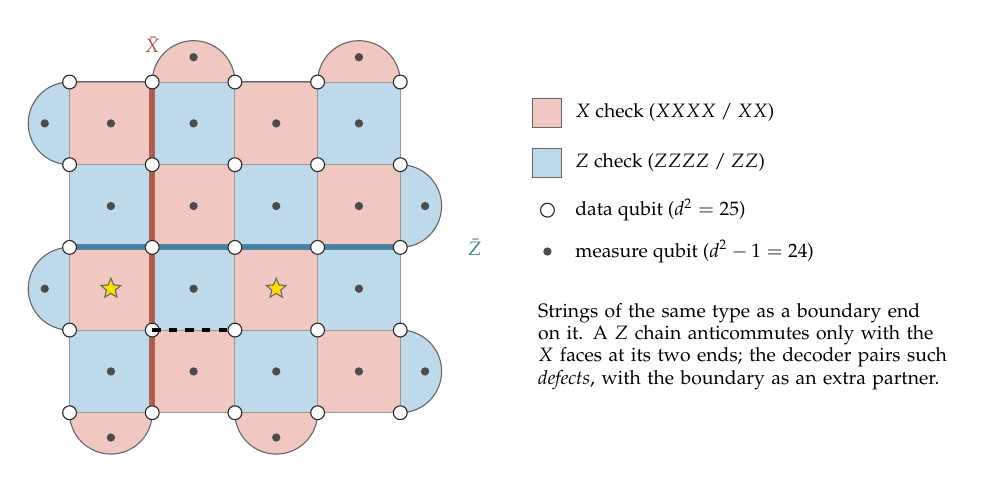
\begin{tikzpicture}[scale=1.05]
\def\d{5}
% bulk faces
\foreach \i in {0,...,3}{\foreach \j in {0,...,3}{
  \pgfmathparse{int(mod(\i+\j,2))}
  \ifnum\pgfmathresult=0
    \fill[xface] (\j,-\i) rectangle (\j+1,-\i-1);
  \else
    \fill[zface] (\j,-\i) rectangle (\j+1,-\i-1);
  \fi}}
% boundary half-discs: top X at columns 1-2 and 3-4 ; bottom X at 0-1 and 2-3; left Z rows 0-1, 2-3 ; right Z rows 1-2, 3-4
\foreach \j in {1,3}{\fill[xface] (\j+1,0) arc (0:180:0.5);}
\foreach \j in {0,2}{\fill[xface] (\j,-4) arc (180:360:0.5);}
\foreach \i in {0,2}{\fill[zface] (0,-\i) arc (90:270:0.5);}
\foreach \i in {1,3}{\fill[zface] (4,-\i-1) arc (270:450:0.5);}
% grid lines
\draw[black!40,thin] (0,0) grid[step=1] (4,-4);
% logical operators
\draw[line width=2.2pt,cZ!80!black,opacity=0.85] (0,-2) -- (4,-2);
\node[font=\scriptsize,text=cZ!80!black] at (4.9,-2) {$\bar Z$};
\draw[line width=2.2pt,cX!80!black,opacity=0.85] (1,0) -- (1,-4);
\node[font=\scriptsize,text=cX!80!black] at (1,0.45) {$\bar X$};
% data qubits
\foreach \i in {0,...,4}{\foreach \j in {0,...,4}{\node[dq] at (\j,-\i) {};}}
% measure qubits (face centres)
\foreach \i in {0,...,3}{\foreach \j in {0,...,3}{\node[circle,fill=black!70,inner sep=0pt,minimum size=3pt] at (\j+0.5,-\i-0.5) {};}}
\foreach \j in {1,3}{\node[circle,fill=black!70,inner sep=0pt,minimum size=3pt] at (\j+0.5,0.3) {};}
\foreach \j in {0,2}{\node[circle,fill=black!70,inner sep=0pt,minimum size=3pt] at (\j+0.5,-4.3) {};}
\foreach \i in {0,2}{\node[circle,fill=black!70,inner sep=0pt,minimum size=3pt] at (-0.3,-\i-0.5) {};}
\foreach \i in {1,3}{\node[circle,fill=black!70,inner sep=0pt,minimum size=3pt] at (4.3,-\i-0.5) {};}
% legend
\fill[xface] (5.6,-0.2) rectangle (5.95,-0.55); \node[font=\scriptsize,anchor=west] at (6.0,-0.37) {$X$ check ($XXXX$ / $XX$)};
\fill[zface] (5.6,-0.8) rectangle (5.95,-1.15); \node[font=\scriptsize,anchor=west] at (6.0,-0.97) {$Z$ check ($ZZZZ$ / $ZZ$)};
\node[dq] at (5.78,-1.55) {}; \node[font=\scriptsize,anchor=west] at (6.0,-1.55) {data qubit ($d^2=25$)};
\node[circle,fill=black!70,inner sep=0pt,minimum size=3pt] at (5.78,-2.05) {}; \node[font=\scriptsize,anchor=west] at (6.0,-2.05) {measure qubit ($d^2-1=24$)};
\node[font=\scriptsize,anchor=west,text width=5.2cm,align=left] at (5.55,-3.2) {Strings of the same type as a boundary end on it. A $Z$ chain anticommutes only with the $X$ faces at its two ends; the decoder pairs such \emph{defects}, with the boundary as an extra partner.};
% an error chain example
\draw[line width=1.6pt,black,dashed] (1,-3) -- (2,-3);
\node[star,star points=5,star point ratio=2.2,fill=yellow!80!orange,draw=black!60,inner sep=1.2pt] at (0.5,-2.5) {};
\node[star,star points=5,star point ratio=2.2,fill=yellow!80!orange,draw=black!60,inner sep=1.2pt] at (2.5,-2.5) {};
\end{tikzpicture}
\caption{The rotated surface code at $d=5$. The dashed chain is a $Z$ error on two neighbouring qubits of the fourth row; the two stars are the only $X$ faces it anticommutes with (the $X$ face between them is touched twice)---the \emph{defects} the decoder sees. The logical operators drawn are the minimum-weight representatives; multiplying $\bar Z$ by any $Z$ face slides it.}
\label{fig:surface-lattice}
\end{figure}

\paragraph{Encoding.} A logical $\ket{0_L}$ is prepared by initialising all data qubits in $\ket0$ and running one cycle of syndrome measurement: the $Z$ faces are already satisfied, the $X$ faces return random outcomes that are simply recorded as the reference frame (or fixed by $Z$ corrections), and from then on the code is live. $\ket{+_L}$ is the same with $\ket+$ and the $X$ faces. Reading out $\bar Z$ is the time-reversed operation: measure every data qubit in the $Z$ basis, recompute the $Z$ faces from the outcomes to get one last syndrome round (so that the readout itself is error-corrected), and take the parity along any $\bar Z$ string.

\paragraph{Syndrome extraction.} Each face has one measurement qubit. One cycle (\cref{fig:surface-cycle}) is: reset the ancillas; Hadamard the $X$-face ancillas; four layers of CNOTs in which every face talks to its four corners in a fixed order; Hadamard; measure. The order matters because of \emph{hook errors}: an ancilla fault between the second and third CNOT propagates to the last two data qubits of the order, and if that pair were aligned with the logical operator the pair would count as a single fault that advances a chain by two, halving the effective distance. The standard orders---``Z'' shape (NW, NE, SW, SE) for the $X$ faces and ``N'' shape (NW, SW, NE, SE) for the $Z$ faces---make every hook pair perpendicular to the logical string it could have helped, and they also let all faces run their CNOTs simultaneously, because at each layer every data qubit is touched by exactly one face. The whole cycle is $8$ layers; Google's Willow runs it in $1.1\,\mu$s \cite{willow25}, which is the ``$1\,\mu$s cycle'' of every superconducting estimate in \cref{sec:physical}.

\begin{figure}[H]
\centering
\begin{quantikz}[column sep=6pt,row sep=4pt,font=\small]
\lstick{$X$-face ancilla $\ket0$} & \gate{H} & \ctrl{1} & \ctrl{2} & \ctrl{3} & \ctrl{4} & \gate{H} & \meter{} \\
\lstick{NW} & \qw & \targ{} & \qw & \qw & \qw & \qw & \qw \\
\lstick{NE} & \qw & \qw & \targ{} & \qw & \qw & \qw & \qw \\
\lstick{SW} & \qw & \qw & \qw & \targ{} & \qw & \qw & \qw \\
\lstick{SE} & \qw & \qw & \qw & \qw & \targ{} & \qw & \qw
\end{quantikz}
\hspace{6mm}
\begin{quantikz}[column sep=6pt,row sep=4pt,font=\small]
\lstick{$Z$-face ancilla $\ket0$} & \qw & \targ{} & \targ{} & \targ{} & \targ{} & \qw & \meter{} \\
\lstick{NW} & \qw & \ctrl{-1} & \qw & \qw & \qw & \qw & \qw \\
\lstick{SW} & \qw & \qw & \ctrl{-2} & \qw & \qw & \qw & \qw \\
\lstick{NE} & \qw & \qw & \qw & \ctrl{-3} & \qw & \qw & \qw \\
\lstick{SE} & \qw & \qw & \qw & \qw & \ctrl{-4} & \qw & \qw
\end{quantikz}
\caption{One surface-code cycle for an $X$ face (left, order NW--NE--SW--SE) and a $Z$ face (right, order NW--SW--NE--SE). The four CNOT layers of all faces run in parallel; the hook pairs (last two targets) are horizontal for $X$ faces and vertical for $Z$ faces, perpendicular to $\bar X$ and $\bar Z$ respectively in \cref{fig:surface-lattice}.}
\label{fig:surface-cycle}
\end{figure}

\subsubsection{Decoding the surface code}\label{sec:mwpm}
Because measurements are noisy, one round is never enough: the cycle is repeated, and the decoder works on \emph{detectors}, the XOR of consecutive outcomes of the same face \cite{dennis02}. In the resulting three-dimensional space-time picture (\cref{fig:matching}), every elementary fault flips at most two detectors: a data error between rounds flips the two faces beside it (a space-like edge), a measurement error flips the same face in two consecutive rounds (a time-like edge), a CNOT fault or hook flips a diagonal pair (a space-time edge), and a fault next to a boundary flips a single detector (an edge to the boundary node). The \emph{detector error model} is the list of these edges with their probabilities; Stim derives it from the circuit, and \cref{fig:threshold} was produced that way \cite{gidney21stim}. Decoding then means choosing a set of edges that explains the observed defects and is most probable:

\begin{algorithm}[H]
\caption{Minimum-weight perfect matching (MWPM) decoding of a surface-code memory}\label{alg:mwpm}
\begin{algorithmic}[1]
\Require detector error model $G=(V,E)$ with edge probabilities $p_e$ and logical-flip labels; observed defect set $D\subseteq V$ (odd $|D|$ is made even by a boundary node)
\State weight every edge $w_e=\log\frac{1-p_e}{p_e}$ (so that a path's weight is $-\log$ of its probability up to a constant)
\State for every pair of defects, the lightest path between them is the shortest path in $(G,w)$ (Dijkstra); build the complete graph on $D$ with these distances, plus a boundary partner per defect
\State find a \emph{perfect matching} of minimum total weight (Edmonds' blossom algorithm; sparse blossom explores the paths lazily and runs in near-linear time at low $p$ \cite{higgott23pymatching})
\State the correction is the XOR of the matched paths' logical labels: the decoder never touches the qubits, it flips the Pauli frame
\end{algorithmic}
\end{algorithm}

MWPM finds the single most likely error, not the most likely \emph{class} of errors; it ignores degeneracy and the correlations between $X$ and $Z$ decoding caused by $Y$ errors, and each of those costs a little threshold. Fowler showed that matching can be made $O(1)$ average time per round with parallel hardware \cite{fowler13mwpm}; PyMatching's sparse blossom decodes about a million detection events per second per core \cite{higgott23pymatching}; Google's real-time decoder kept up with the $1.1\,\mu$s cycle of a distance-$5$ memory for a million cycles with $63\,\mu$s average latency \cite{willow25}, and \emph{latency}, not throughput, is what sets the reaction time that multiplies every non-Clifford gate in \cref{sec:physical}.

\begin{figure}[H]
\centering
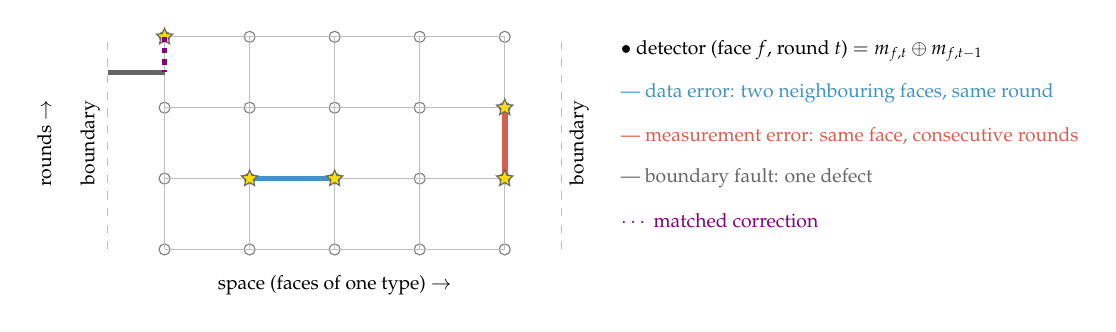
\begin{tikzpicture}[scale=0.9]
% space-time lattice of detectors for one face-type: 5 columns x 4 rounds
\foreach \t in {0,...,3}{\foreach \x in {0,...,4}{\node[circle,draw=black!50,fill=white,inner sep=0pt,minimum size=4pt] (n\x\t) at (\x*1.2,\t*1.0) {};}}
\foreach \t in {0,...,3}{\draw[black!25] (0,\t) -- (4.8,\t);}
\foreach \x in {0,...,4}{\draw[black!25] (\x*1.2,0) -- (\x*1.2,3);}
\draw[black!25,dashed] (-0.8,0) -- (-0.8,3); \node[font=\scriptsize,rotate=90] at (-1.05,1.5) {boundary};
\draw[black!25,dashed] (5.6,0) -- (5.6,3); \node[font=\scriptsize,rotate=90] at (5.85,1.5) {boundary};
% faults: data error at t=1 between x=1 and x=2 -> defects (1,1),(2,1)
\draw[cZ,line width=2pt] (1.2,1) -- (2.4,1);
\node[star,star points=5,star point ratio=2.2,fill=yellow!80!orange,draw=black!60,inner sep=1pt] at (1.2,1) {};
\node[star,star points=5,star point ratio=2.2,fill=yellow!80!orange,draw=black!60,inner sep=1pt] at (2.4,1) {};
% measurement error at x=4 between t=1 and t=2 -> defects (4,1),(4,2)
\draw[cX,line width=2pt] (4.8,1) -- (4.8,2);
\node[star,star points=5,star point ratio=2.2,fill=yellow!80!orange,draw=black!60,inner sep=1pt] at (4.8,1) {};
\node[star,star points=5,star point ratio=2.2,fill=yellow!80!orange,draw=black!60,inner sep=1pt] at (4.8,2) {};
% hook / space-time diagonal at x=0: t=2 -> boundary edge
\draw[black!60,line width=2pt] (0,2.5) -- (-0.8,2.5);
\node[star,star points=5,star point ratio=2.2,fill=yellow!80!orange,draw=black!60,inner sep=1pt] at (0,3) {};
\draw[violet,line width=2pt,dotted] (0,3) -- (0,2.5);
\node[font=\scriptsize,anchor=west] at (6.3,2.8) {$\bullet$ detector (face $f$, round $t$) $=m_{f,t}\oplus m_{f,t-1}$};
\node[font=\scriptsize,anchor=west,text=cZ] at (6.3,2.2) {--- data error: two neighbouring faces, same round};
\node[font=\scriptsize,anchor=west,text=cX] at (6.3,1.6) {--- measurement error: same face, consecutive rounds};
\node[font=\scriptsize,anchor=west,text=black!60] at (6.3,1.0) {--- boundary fault: one defect};
\node[font=\scriptsize,anchor=west,text=violet] at (6.3,0.4) {$\cdots$ matched correction};
\node[font=\scriptsize] at (2.4,-0.5) {space (faces of one type) $\rightarrow$};
\node[font=\scriptsize,rotate=90] at (-1.7,1.5) {rounds $\rightarrow$};
\end{tikzpicture}
\caption{The decoding graph of one check type over four rounds: every fault is an edge, every defect a vertex, and MWPM pairs the defects by lightest edges. A chain of faults that crosses the whole patch (or a matched correction that does) flips the logical operator.}
\label{fig:matching}
\end{figure}

\paragraph{Union-find.}\label{sec:unionfind} Delfosse and Nickerson's decoder \cite{delfosse-nickerson21} trades a little accuracy for almost-linear worst-case time ($O(n\,\alpha(n))$, $\alpha$ the inverse Ackermann function) and a structure that maps to simple hardware:

\begin{algorithm}[H]
\caption{Union-find decoder}\label{alg:uf}
\begin{algorithmic}[1]
\State start one cluster per defect; a cluster is \emph{odd} if it contains an odd number of defects and does not touch the boundary
\While{some cluster is odd}
  \State grow every odd cluster by half an edge in all directions (\emph{syndrome validation})
  \State when two clusters touch, merge them (union-find with path compression keeps this near constant time); a merged cluster's parity is the sum
\EndWhile
\State inside each cluster, build a spanning forest and \emph{peel} it from the leaves: remove a leaf edge, flip it in the correction iff the leaf vertex is an unmatched defect, and toggle the parity of the other endpoint
\end{algorithmic}
\end{algorithm}
Its threshold is a few tenths of a percent below MWPM's under the same noise, which is why it is used where decoding hardware is the constraint and why many real-time decoders start from it.

\paragraph{Learned decoders.} AlphaQubit \cite{alphaqubit24} (Google DeepMind and Google Quantum AI) is a recurrent transformer trained first on simulated data and then fine-tuned on Sycamore syndrome records; it beat correlated matching on the experimental distance-$3$ and $-5$ data by using the soft measurement information and the device's real error correlations, at the price of a latency that is not yet compatible with real-time use.

\subsubsection{The threshold, measured}\label{sec:threshold}
\Cref{fig:threshold} is a circuit-level simulation performed for this document with Stim and PyMatching (\code{surface\_threshold.py}, \cref{app:scripts}): rotated memory-$Z$ patches of distance $3$--$9$, $d$ rounds each, uniform depolarising noise of strength $p$ after every Clifford, before every round on the data, and on every measurement and reset; at least $1{,}000$ logical failures or $12$ million shots per point; the logical error per shot $\epsilon$ converted to an error per round by $\epsilon_{\rm round}=\frac12(1-(1-2\epsilon)^{1/d})$. The curves cross at $p\approx1.1$--$1.2\%$, the circuit-level threshold under this noise model; below it, each $+2$ of distance divides the error by $\Lambda$, which the data put at $\Lambda\approx9.6$, $10.6$ and $14.8$ for the steps $3\to5$, $5\to7$ and $7\to9$ at $p=10^{-3}$, $\approx5$ at $p=2\times10^{-3}$ and $\approx3.2$ at $p=3\times10^{-3}$. Google's Willow reached $\Lambda=2.14\pm0.02$ with a $d=7$ logical error of $0.143\%$ per cycle on $101$ qubits, which in this uniform model corresponds to $p\approx0.45\%$ (real noise is far from uniform: Willow's two-qubit gates are better than that, its measurements worse); the $\Lambda\approx10$ of the $p=10^{-3}$ estimates is a factor four or five in physical error away from that device \cite{willow25}.

\begin{figure}[H]
\centering
\begin{tikzpicture}
\begin{loglogaxis}[width=0.62\textwidth,height=0.5\textwidth,
  xlabel={physical error rate $p$ (circuit-level depolarising)}, ylabel={logical error per round $\epsilon_{\rm round}$},
  xmin=0.0004,xmax=0.02,ymin=1e-8,ymax=0.2, grid=both,grid style={black!10},
  legend style={font=\scriptsize,at={(0.03,0.97)},anchor=north west,cells={anchor=west}},
  tick label style={font=\footnotesize},label style={font=\small},
  xtick={0.0005,0.001,0.002,0.005,0.01,0.02}, xticklabels={$0.05\%$,$0.1\%$,$0.2\%$,$0.5\%$,$1\%$,$2\%$}]
\addplot[color=cZ!70!black,mark=*,mark size=1.4pt,thick] table[x=p,y=eps_round,discard if not={d}{3}] {data/surface_threshold.dat}; \addlegendentry{$d=3$}
\addplot[color=boxgreen,mark=square*,mark size=1.4pt,thick] table[x=p,y=eps_round,discard if not={d}{5}] {data/surface_threshold.dat}; \addlegendentry{$d=5$}
\addplot[color=orange!85!black,mark=triangle*,mark size=1.8pt,thick] table[x=p,y=eps_round,discard if not={d}{7}] {data/surface_threshold.dat}; \addlegendentry{$d=7$}
\addplot[color=boxred,mark=diamond*,mark size=1.8pt,thick] table[x=p,y=eps_round,discard if not={d}{9}] {data/surface_threshold.dat}; \addlegendentry{$d=9$}
\draw[black!50,dashed] (axis cs:0.001,1e-8) -- (axis cs:0.001,0.2);
\node[font=\scriptsize,anchor=south west,rotate=90] at (axis cs:0.001,2e-8) {$p=10^{-3}$ (Model S)};
\draw[black!50,dashed] (axis cs:0.0115,1e-8) -- (axis cs:0.0115,0.2);
\node[font=\scriptsize,anchor=south east,rotate=90] at (axis cs:0.0115,2e-8) {crossing $\approx1.15\%$};
\end{loglogaxis}
\end{tikzpicture}
\hfill
\begin{minipage}[b]{0.34\textwidth}\footnotesize\centering
\begin{tabular}{@{}lccc@{}}\toprule
$p$ & $\Lambda_{3\to5}$ & $\Lambda_{5\to7}$ & $\Lambda_{7\to9}$\\\midrule
$10^{-3}$ & 9.6 & 10.6 & 14.8\\
$2\times10^{-3}$ & 5.3 & 4.8 & 5.0\\
$3\times10^{-3}$ & 3.3 & 3.2 & 3.2\\
$5\times10^{-3}$ & 2.0 & 1.9 & 1.9\\\bottomrule
\end{tabular}\\[4pt]
$\epsilon_{\rm round}(d{=}9,p{=}10^{-3})=1.7\times10^{-7}$ ($18$ failures)\\
extrapolated to $d=25$ at $\Lambda\approx10$: $\approx10^{-15}$\\[6pt]
\end{minipage}
\caption{Surface-code threshold computed for this document (\cref{app:scripts}). Left: logical error per round against physical error for four distances; the crossing is the threshold. Right: the suppression factor $\Lambda$ between successive distances, read off the same data; the extrapolation to $d=25$ uses $\Lambda\approx10$ per step, consistent with \cref{eq:plaw} at $p_{\rm th}\approx1.2\%$. Points with fewer than $200$ failures ($d=7,9$ at $p\le10^{-3}$) carry $\pm10$--$25\%$ statistical error; the $d=9$ point at $p=0.05\%$ had no failure in $12$ million shots and is not drawn.}
\label{fig:threshold}
\end{figure}

\paragraph{Lattice surgery and logical gates.} The surface code has no transversal gate beyond the Paulis, so its logical CNOTs, Hadamards and measurements are made by merging and splitting patches---\emph{lattice surgery}---and its $T$ gates by consuming magic states; both are in \cref{sec:ft-clifford,sec:ft-t}.

\section{The codes: colour codes and quantum LDPC codes}\label{sec:codes2}

\subsection{Colour codes}\label{sec:colour}

\subsubsection{Two-dimensional colour codes}
Take a trivalent lattice whose faces can be three-coloured so that no two faces of the same colour share an edge (the $4.8.8$ tiling of squares and octagons, or the $6.6.6$ honeycomb), put a qubit on every vertex, and attach to every face \emph{both} an $X$-type and a $Z$-type check on its vertices \cite{bombin06}. Two faces share $0$ or $2$ vertices (trivalence plus three-colourability), so all checks commute, and the code is CSS with $H_X=H_Z$: it is \emph{self-dual}. A triangular patch with one boundary of each colour encodes one qubit; the $4.8.8$ family has $n=\frac{d^2+2d-1}2$ ($7,17,31,49,\dots$) and the $6.6.6$ family $n=\frac{3d^2+1}4$ ($7,19,37,\dots$); both start at the Steane code (\cref{fig:colour}). Because $H_X=H_Z$, transversal Hadamard $H^{\otimes n}$ swaps the two check families and so preserves the code, implementing $\bar H$; and because every face has a number of vertices divisible by four---every stabiliser weight is doubly even---the transversal $S^{\otimes n}$ (or $S^{\dagger\otimes n}$) is a logical $S$ \cite{kubica15}. With the transversal CNOT of any CSS code this is the whole Clifford group, transversally, in two dimensions: the colour code is the natural home of the Clifford frame (\cref{sec:ft-clifford}).

\begin{figure}[H]
\centering
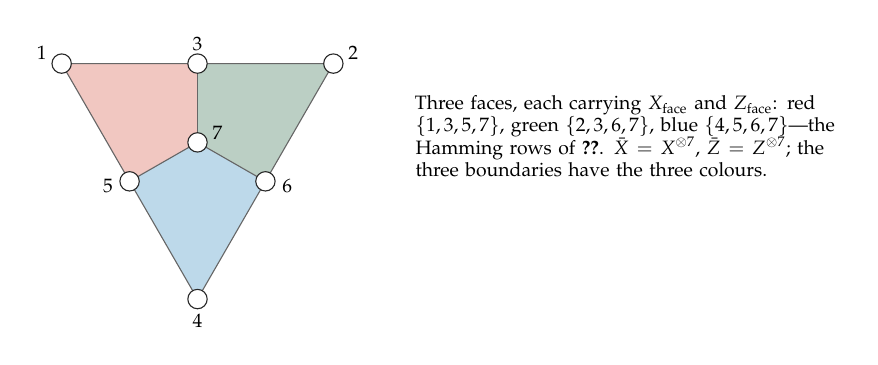
\begin{tikzpicture}[scale=1.15]
\coordinate (q1) at (-1.5,1); \coordinate (q2) at (1.5,1); \coordinate (q4) at (0,-1.6);
\coordinate (q3) at (0,1); \coordinate (q5) at (-0.75,-0.3); \coordinate (q6) at (0.75,-0.3); \coordinate (q7) at (0,0.13);
\fill[cX!35] (q7) -- (q3) -- (q1) -- (q5) -- cycle;
\fill[boxgreen!30] (q7) -- (q3) -- (q2) -- (q6) -- cycle;
\fill[cZ!35] (q7) -- (q5) -- (q4) -- (q6) -- cycle;
\draw[black!60] (q1) -- (q2) -- (q4) -- cycle; \draw[black!60] (q7) -- (q3); \draw[black!60] (q7) -- (q5); \draw[black!60] (q7) -- (q6);
\foreach \n/\l in {q1/1,q2/2,q3/3,q4/4,q5/5,q6/6,q7/7}{\node[dq,minimum size=7pt] at (\n) {}; }
\node[font=\scriptsize] at ($(q1)+(-0.22,0.12)$) {1}; \node[font=\scriptsize] at ($(q2)+(0.22,0.12)$) {2}; \node[font=\scriptsize] at ($(q3)+(0,0.22)$) {3};
\node[font=\scriptsize] at ($(q4)+(0,-0.24)$) {4}; \node[font=\scriptsize] at ($(q5)+(-0.24,-0.05)$) {5}; \node[font=\scriptsize] at ($(q6)+(0.24,-0.05)$) {6}; \node[font=\scriptsize] at ($(q7)+(0.22,0.1)$) {7};
\node[font=\scriptsize,text width=5.4cm,anchor=west] at (2.3,0.2) {Three faces, each carrying $X_{\rm face}$ and $Z_{\rm face}$: red $\{1,3,5,7\}$, green $\{2,3,6,7\}$, blue $\{4,5,6,7\}$---the Hamming rows of \cref{tab:syn-steane}. $\bar X=X^{\otimes7}$, $\bar Z=Z^{\otimes7}$; the three boundaries have the three colours.};
\end{tikzpicture}
\hspace{4mm}
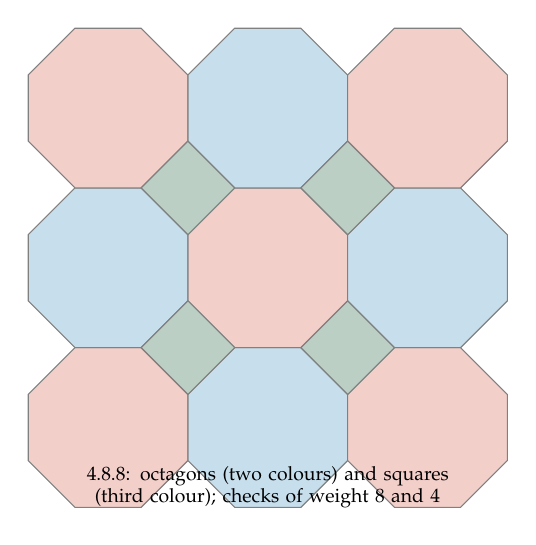
\begin{tikzpicture}[scale=0.42]
% a 4.8.8 fragment: octagons at (0,0),(4,4)... draw a 3x3 block of octagons with squares in between
\foreach \i in {0,1,2}{\foreach \j in {0,1,2}{
  \pgfmathsetmacro{\cx}{\i*4.83}\pgfmathsetmacro{\cy}{\j*4.83}
  \pgfmathparse{int(mod(\i+\j,2))}
  \ifnum\pgfmathresult=0 \def\col{cX!30}\else\def\col{cZ!30}\fi
  \fill[\col,draw=black!50] ($(\cx,\cy)+(22.5:2.613)$) \foreach \a in {67.5,112.5,...,382.5}{-- ($(\cx,\cy)+(\a:2.613)$)} -- cycle;
}}
\foreach \i in {0,1}{\foreach \j in {0,1}{
  \pgfmathsetmacro{\cx}{\i*4.83+2.415}\pgfmathsetmacro{\cy}{\j*4.83+2.415}
  \fill[boxgreen!30,draw=black!50] (\cx-1.414,\cy) -- (\cx,\cy+1.414) -- (\cx+1.414,\cy) -- (\cx,\cy-1.414) -- cycle;
}}
\node[font=\scriptsize,text width=4.6cm,align=center] at (4.83,-1.8) {$4.8.8$: octagons (two colours) and squares (third colour); checks of weight 8 and 4};
\end{tikzpicture}
\caption{Left: the $\bits{7}{1}{3}$ code as the smallest triangular colour code. Right: a fragment of the $4.8.8$ lattice from which the $\bits{17}{1}{5}$, $\bits{31}{1}{7}$, \dots\ codes of \cref{fig:bounds} are cut.}
\label{fig:colour}
\end{figure}

The price is paid in decoding and in threshold. A single error flips \emph{three} checks (one of each colour), so the decoding graph is a hypergraph and matching does not apply directly. Delfosse's \emph{projection} (restriction) decoder \cite{delfosse14} restricts the syndrome to the two colours $\{c_1,c_2\}$---where every error flips exactly two of the remaining checks---runs MWPM on that surface-code-like sub-problem, repeats for the other pairs, and lifts the three matchings to a colour-code correction; the \emph{M\"obius} decoder and Google's open-source Chromobius refine the lift \cite{gidney23color}. Syndrome extraction is also heavier: a weight-eight octagon needs eight CNOTs and the hook problem of \cref{fig:surface-cycle} is harder to tame, which is what the ``superdense'' and ``middle-out'' cycles of Gidney and Jones address. The result is that at $p=0.1\%$ a colour code needs about $1{,}250$ physical qubits for a $10^{-12}$-per-round logical qubit (the \emph{teraquop footprint}) where the surface code with correlated matching needs $650$ \cite{gidney23color}; Google's 2024 experiment measured $\Lambda_{3/5}=1.56(4)$ on a colour code, transversal Clifford gates adding only $0.0027(3)$ error per operation, magic-state injection above $99\%$ with $75\%$ post-selection yield, and lattice surgery between $d=3$ patches \cite{lacroix24color}. Honeywell/Quantinuum's $\bits{7}{1}{3}$ demonstrations---real-time error correction in 2021, fault-tolerant logical teleportation with transversal gates and lattice surgery in 2024---are colour-code experiments \cite{ryan-anderson21,ryan-anderson24}.

\subsubsection{Three-dimensional colour codes, gauge colour codes}
On a three-dimensional four-colourable lattice, with $X$-checks on the \emph{cells} and $Z$-checks on the \emph{faces}, every $X$-stabiliser is triply even and the code has a transversal $T$ \cite{bombin07,kubica15}; the tetrahedral $d=3$ member is the $\bits{15}{1}{3}$ code of \cref{sec:smallcodes}. By the Bravyi--K\"onig theorem a $D$-dimensional topological code can only have transversal gates in level $D$ of the Clifford hierarchy, so 3D is the minimum for a transversal $T$ and no such code has a transversal $H$ as well \cite{bravyi-koenig13}. Bomb\'in's \emph{gauge colour code} \cite{bombin15} places both $X$- and $Z$-type operators on faces into a gauge group; fixing the gauge one way yields the code with transversal $T$, fixing it the other way yields a code with transversal Clifford gates, and switching between the two by measuring the gauge operators of the target code is the \emph{gauge fixing} route to universality of \cref{sec:codeswitch}. The 3D code also allows \emph{single-shot} error correction (one noisy syndrome round suffices, because the cell checks are redundant and their redundancy corrects measurement errors), but its qubit count grows as $d^3$.

\subsection{Quantum LDPC codes}\label{sec:qldpc}

A family of codes is \emph{LDPC} if every check has bounded weight and every qubit is in a bounded number of checks as $n\to\infty$; the surface code is LDPC with weight $4$, but with $k=1$. The hope of the field, and the design basis of IBM's, IonQ's and the neutral-atom roadmaps, is codes that are LDPC \emph{and} have $k=\Theta(n)$ (constant rate) with $d$ growing as fast as possible---which by the BPT bound \eqref{eq:bpt} requires long-range checks \cite{breuckmann-eberhardt21}. Constructing such codes is a problem of commuting checks: random sparse $H_X,H_Z$ never satisfy $H_XH_Z^{\mathsf T}=0$, so every construction builds the orthogonality in algebraically.

\subsubsection{Hypergraph product codes}
Tillich and Z\'emor's product \cite{tillich-zemor14} takes two classical parity-check matrices $H_1$ ($m_1\times n_1$) and $H_2$ ($m_2\times n_2$) and sets
\begin{equation}\label{eq:hgp}
H_X=\big[\,H_1\otimes I_{n_2}\ \big|\ I_{m_1}\otimes H_2^{\mathsf T}\,\big],\qquad
H_Z=\big[\,I_{n_1}\otimes H_2\ \big|\ H_1^{\mathsf T}\otimes I_{m_2}\,\big],
\end{equation}
so that $H_XH_Z^{\mathsf T}=H_1\otimes H_2^{\mathsf T}+H_1\otimes H_2^{\mathsf T}=0$ automatically. The qubits are the $n_1n_2$ ``bit--bit'' pairs plus the $m_1m_2$ ``check--check'' pairs; the parameters are
\[
\bits{\,n_1n_2+m_1m_2\,}{\,k_1k_2+k_1^{\mathsf T}k_2^{\mathsf T}\,}{\,\min(d_1,d_2,d_1^{\mathsf T},d_2^{\mathsf T})\,},
\]
with $k^{\mathsf T},d^{\mathsf T}$ the dimension and distance of the transpose code $\ker H^{\mathsf T}$. The toric code is the hypergraph product of two cyclic repetition codes ($n_1=n_2=m_1=m_2=L$, $k=1+1=2$, $d=L$). Taking $H_1=H_2$ a good classical LDPC code with $k=\Theta(n)$ and $d=\Theta(n)$ gives $k=\Theta(n)$ and $d=\Theta(\sqrt n)$ quantum codes with constant check weight---the first constant-rate quantum LDPC family---and their generalisation, the \emph{lifted product} over a group ring \cite{panteleev-kalachev21bposd}, is the code family of the neutral-atom estimates in \cref{sec:physical} (e.g.\ $\bits{2610}{744}{\le16}$ at a $29\%$ rate) \cite{cain26}.

\subsubsection{Bivariate bicycle codes and IBM's gross code}\label{sec:bb}
IBM's bivariate bicycle (BB) codes \cite{bravyi24gross} are the lifted product of a one-term code with itself over the abelian group $\Z_\ell\times\Z_m$. Let $x=S_\ell\otimes I_m$ and $y=I_\ell\otimes S_m$ be the two commuting cyclic-shift matrices ($S_\ell$ the $\ell\times\ell$ shift), and let $A$ and $B$ be sums of three monomials in $x,y$. Then
\begin{equation}\label{eq:bb}
H_X=[\,A\ |\ B\,],\qquad H_Z=[\,B^{\mathsf T}\ |\ A^{\mathsf T}\,],\qquad H_XH_Z^{\mathsf T}=AB+BA=0,
\end{equation}
because polynomials in commuting matrices commute. There are $n=2\ell m$ data qubits in two halves $L$ and $R$, $\ell m$ $X$-checks and $\ell m$ $Z$-checks, every check has weight six (three $L$ neighbours from the monomials of $A$ or $B^{\mathsf T}$, three $R$ neighbours from the other), every data qubit is in three $X$- and three $Z$-checks, and $k=2\dim(\ker A\cap\ker B)$. \Cref{tab:bb} lists the codes of IBM's paper; the parameters $n$, $k$, check weights and degrees were recomputed for this document from the polynomials (\code{scripts/bb\_codes.py}), the distances are IBM's (found by integer programming).

\begin{table}[H]
\centering\footnotesize
\begin{tabular}{@{}lccllc@{}}
\toprule
code & $\ell,m$ & $n$ & $A$ & $B$ & $k$ (recomputed) \\
\midrule
$\bits{72}{12}{6}$ & $6,6$ & 72 & $x^3+y+y^2$ & $y^3+x+x^2$ & 12\\
$\bits{90}{8}{10}$ & $15,3$ & 90 & $x^9+y+y^2$ & $1+x^2+x^7$ & 8\\
$\bits{108}{8}{10}$ & $9,6$ & 108 & $x^3+y+y^2$ & $y^3+x+x^2$ & 8\\
$\bits{144}{12}{12}$ (``gross'') & $12,6$ & 144 & $x^3+y+y^2$ & $y^3+x+x^2$ & 12\\
$\bits{288}{12}{18}$ (``two-gross'') & $12,12$ & 288 & $x^3+y^2+y^7$ & $y^3+x+x^2$ & 12\\
\bottomrule
\end{tabular}
\caption{Bivariate bicycle codes \cite{bravyi24gross}. Every check has weight $6$ and every qubit degree $6$ (three $X$, three $Z$); $H_XH_Z^{\mathsf T}=0$ and the values of $k$ were verified.}
\label{tab:bb}
\end{table}

\paragraph{Layout and syndrome cycle.} The Tanner graph of a BB code has degree six and is \emph{not} planar, but it is the union of two edge-disjoint planar graphs \cite{bravyi24gross}: on a torus of $\ell\times m$ cells the $L$ qubits, $R$ qubits, $X$-checks and $Z$-checks occupy the four sites of each cell, four of the six edges of every check are nearest-neighbour and two are long-range (the $x^3$, $y^3$ or $x^7$ terms), which is what IBM's \emph{c-couplers} on the Loon processor are for \cite{ibm-blog25}. With one ancilla per check the syndrome cycle is seven CNOT layers deep, interleaving the $X$- and $Z$-check extraction so that a check qubit talks to its six data qubits while the data qubits are shared with the other type; a full cycle is depth $8$ with measurement and reset---the same depth as the surface code's despite the weight-six checks. Under circuit-level depolarising noise with BP+OSD decoding the family has a threshold near $0.8\%$, and at $p=10^{-3}$ the gross code's $288$ qubits hold $12$ logical qubits at a logical error that the surface code would need nearly $3{,}000$ qubits to match: the ``tenfold'' saving \cite{bravyi24gross}. IBM's later circuit and decoder work puts the gross code's idle error at $10^{-8.8}$ per $8$-timestep cycle for the whole block at $p=10^{-3}$, and the two-gross code's at $10^{-20}$ \cite{yoder25tour}.

\begin{figure}[H]
\centering
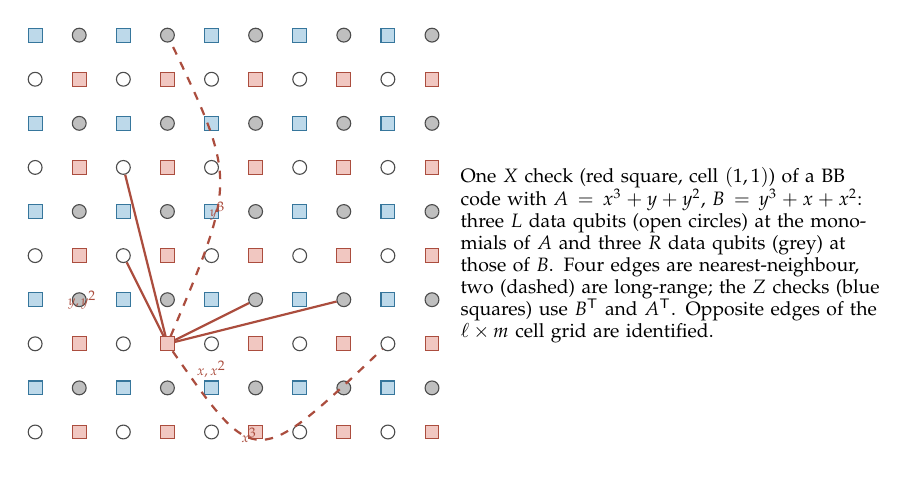
\begin{tikzpicture}[scale=0.8]
\foreach \i in {0,...,4}{\foreach \j in {0,...,4}{
  \node[circle,draw=black!70,fill=white,inner sep=0pt,minimum size=5pt] (L\i\j) at (\i*1.4,\j*1.4) {};
  \node[circle,draw=black!70,fill=black!25,inner sep=0pt,minimum size=5pt] (R\i\j) at (\i*1.4+0.7,\j*1.4+0.7) {};
  \node[rectangle,draw=cX!80!black,fill=cX!35,inner sep=0pt,minimum size=5pt] (X\i\j) at (\i*1.4+0.7,\j*1.4) {};
  \node[rectangle,draw=cZ!80!black,fill=cZ!35,inner sep=0pt,minimum size=5pt] (Z\i\j) at (\i*1.4,\j*1.4+0.7) {};
}}
% X check of cell (1,1): A = x^3 + y + y^2 -> L cells (4,1),(1,2),(1,3); B = y^3 + x + x^2 -> R cells (1,4),(2,1),(3,1)
\draw[cX!80!black,thick] (X11) -- (L12); \draw[cX!80!black,thick] (X11) -- (L13);
\draw[cX!80!black,thick,dashed] (X11) .. controls (3.5,-0.6) .. (L41);
\draw[cX!80!black,thick] (X11) -- (R21); \draw[cX!80!black,thick] (X11) -- (R31);
\draw[cX!80!black,thick,dashed] (X11) .. controls (3.2,4.0) .. (R14);
\node[font=\tiny,text=cX!80!black] at (3.4,-0.05) {$x^3$};
\node[font=\tiny,text=cX!80!black] at (2.9,3.5) {$y^3$};
\node[font=\tiny,text=cX!80!black] at (0.75,2.1) {$y,y^2$};
\node[font=\tiny,text=cX!80!black] at (2.8,1.0) {$x,x^2$};
\node[font=\scriptsize,anchor=west,text width=5.4cm] at (6.6,2.8) {One $X$ check (red square, cell $(1,1)$) of a BB code with $A=x^3+y+y^2$, $B=y^3+x+x^2$: three $L$ data qubits (open circles) at the monomials of $A$ and three $R$ data qubits (grey) at those of $B$. Four edges are nearest-neighbour, two (dashed) are long-range; the $Z$ checks (blue squares) use $B^{\mathsf T}$ and $A^{\mathsf T}$. Opposite edges of the $\ell\times m$ cell grid are identified.};
\end{tikzpicture}
\caption{The bivariate bicycle layout: four sites per unit cell on a torus, degree-six checks, two long-range couplers per check.}
\label{fig:bb-layout}
\end{figure}

\paragraph{Decoding: belief propagation with ordered-statistics post-processing.}\label{sec:bposd}
Quantum LDPC codes are decoded like classical ones, by message passing on the Tanner graph of $H_Z$ (for $X$ errors) and $H_X$ (for $Z$ errors) \cite{roffe20,panteleev-kalachev21bposd}:

\begin{algorithm}[H]
\caption{BP+OSD decoding (one check type; $H$ is $m\times n$, syndrome $s$, prior error rate $p$)}\label{alg:bposd}
\begin{algorithmic}[1]
\State initialise every variable-to-check message with the prior log-likelihood ratio $\lambda_0=\log\frac{1-p}{p}$
\For{$t=1,\dots,T_{\max}$}\Comment{min-sum belief propagation}
  \State check $i$ to variable $j$: $\mu_{i\to j}=(-1)^{s_i}\,\alpha\prod_{j'\in N(i)\setminus j}\mathrm{sgn}(\lambda_{j'\to i})\cdot\min_{j'\in N(i)\setminus j}|\lambda_{j'\to i}|$ (scaling $\alpha\approx0.8$)
  \State variable $j$ to check $i$: $\lambda_{j\to i}=\lambda_0+\sum_{i'\in N(j)\setminus i}\mu_{i'\to j}$;\quad posterior $\Lambda_j=\lambda_0+\sum_{i'\in N(j)}\mu_{i'\to j}$
  \State hard decision $\hat e_j=[\Lambda_j<0]$; \textbf{if} $H\hat e=s$ \textbf{return} $\hat e$
\EndFor
\State \textbf{OSD-0:} sort the columns of $H$ by increasing $\Lambda_j$ (most likely error first); Gaussian-eliminate in that order to pick an information set $S$ of $\rank H$ independent columns; solve $H_S\,e_S=s$ and set $e_j=0$ off $S$; \textbf{return} $e$
\State \textbf{OSD-CS($\lambda$)} (optional): also try flipping each of the next $\lambda$ most-likely columns outside $S$, one or two at a time, re-solving each time, and keep the lowest-weight solution
\end{algorithmic}
\end{algorithm}

Plain BP fails on quantum codes far more often than on classical ones because of degeneracy: two equally likely errors that differ by a stabiliser pull the marginals in opposite directions, the messages oscillate, and BP ends in a configuration that does not satisfy the syndrome. OSD repairs exactly that case, at the cost of an $O(n^3)$ elimination, which is why decoding \emph{speed} is the main engineering problem of qLDPC architectures. \Cref{fig:bposd} is a small BP+OSD-0 simulation of the gross code written for this document (code-capacity bit-flip noise, i.e.\ no measurement errors, which is far easier than circuit-level noise and only illustrates the decoder); IBM's answer to the speed problem is \textbf{Relay-BP} \cite{mueller25relaybp}: BP with \emph{disordered memory strengths} (each variable node mixes its new belief with its previous one by a node-dependent, partly negative weight, which damps the oscillations and breaks the symmetries that trap plain BP), run as a \emph{relay} of several short BP instances with different memory settings that hand their beliefs on, so that several valid corrections are found and the best kept. On BB codes under circuit noise it outperforms BP+OSD with combination sweep, on surface codes it matches MWPM, and it is a parallel message-passing algorithm that fits an FPGA or ASIC---IBM quotes a $5$--$10\times$ reduction in decoding resources \cite{ibm-blog25}. Cain et al.'s neutral-atom estimates use BP with \emph{localised statistics} decoding in the same spirit \cite{cain26}.

\begin{figure}[H]
\centering
\begin{tikzpicture}
\begin{loglogaxis}[width=0.6\textwidth,height=0.42\textwidth,
  xlabel={bit-flip probability $p$ per data qubit}, ylabel={logical failure per block (12 qubits)},
  xmin=0.015,xmax=0.12,ymin=5e-4,ymax=1, grid=both,grid style={black!10},
  legend style={font=\scriptsize,at={(0.03,0.97)},anchor=north west,cells={anchor=west}},
  tick label style={font=\footnotesize},label style={font=\small},
  xtick={0.02,0.03,0.05,0.1}, xticklabels={$2\%$,$3\%$,$5\%$,$10\%$}]
\addplot[color=violet,mark=diamond*,mark size=2pt,thick] table[x=p,y=pL] {data/bb_bposd.dat}; \addlegendentry{gross code, min-sum BP ($60$ it.) + OSD-0}
\addplot[color=black!50,dashed,domain=0.015:0.12] {x}; \addlegendentry{$p_L=p$ (pseudo-threshold)}
\end{loglogaxis}
\end{tikzpicture}
\caption{BP+OSD-0 on the $\bits{144}{12}{12}$ gross code under independent $X$ errors (computed; $1{,}000$--$2{,}000$ trials per point, \code{scripts/bp\_osd\_gross.py}). The block fails when the residual error is outside the $X$-stabiliser group. Code-capacity noise only; the circuit-level numbers of \cite{bravyi24gross,yoder25tour} are orders of magnitude lower at $p=10^{-3}$.}
\label{fig:bposd}
\end{figure}

\paragraph{Logical operations and IBM's bicycle architecture.} A BB code has no boundaries to merge, so lattice surgery is replaced by two mechanisms. First, the shifts $x$ and $y$ are \emph{automorphisms}: permuting the qubits by $x^ay^b$ maps the code to itself and acts as a logical Clifford on the $12$ logical qubits (together with the $L\leftrightarrow R$ ``ZX-duality'' that swaps $H_X$ and $H_Z$); IBM's instruction set has twelve such shift automorphisms, each a physical permutation (SWAP network) that costs $14$ timesteps \cite{yoder25tour}. Second, arbitrary logical Pauli measurements are made by \emph{generalised surgery} \cite{cohen22,cross24surgery}: to measure a logical $\bar P$ one attaches an auxiliary system of ancilla qubits whose checks, together with the code's, form a temporarily larger code in which $\bar P$ is a product of new stabilisers; measuring the enlarged code for $\approx d$ rounds measures $\bar P$ fault-tolerantly, and the ancillas are then released. IBM's improved construction needs only $\Theta(w)$ ancillas for a weight-$w$ logical and gives the gross code its \emph{logical processing unit} (LPU): $90$ extra qubits (158 for two-gross) wired to the code block through which any Pauli in a chosen generating set can be measured, with one of the twelve logical qubits used as a workspace, so that all logical Cliffords are reachable \cite{cross24surgery,yoder25tour}. A \emph{bicycle module} is then a code block ($288$ or $576$ qubits), its LPU, a $22$-qubit code-to-code adapter for inter-module joint measurements, and a magic-state factory ($454$ qubits at $p=10^{-3}$) with a $29$-qubit adapter; in-module logical measurements cost $120$ timesteps at $10^{-5.0}$ error (gross) or $216$ timesteps at $\approx10^{-11}$ (two-gross), $T$ injection is a joint $\bar Z_T\otimes\bar P$ measurement between factory and module followed by an $\bar X_T$ readout, and IBM estimates that for a given number of physical qubits the architecture runs circuits about ten times larger than a surface-code machine \cite{yoder25tour}. The roadmap built on it \cite{ibm-blog25,ibm-roadmap}: Loon (2025) tests the c-couplers; Kookaburra (2026) is the first module with a qLDPC memory and an LPU; Cockatoo (2027) entangles two modules through the adapter; Starling (2029) targets $200$ logical qubits and $10^8$ gates; Blue Jay ($2033$) $2{,}000$ logical qubits and $10^9$ gates. IBM's Quantum Learning course on error correction is the pedagogical companion to these papers \cite{ibm-learning-qec}.

\subsubsection{Trapped ions: IonQ's walking-cat architecture}\label{sec:ionq-arch}
Trapped ions have no fixed connectivity---ions are shuttled between zones---so the locality constraint that shapes the superconducting designs disappears, and IonQ's architecture \cite{walkingcat26} uses quantum LDPC codes with Shor-style syndrome extraction: a \emph{cat factory} continuously prepares and verifies GHZ (cat) states, which are physically transported (``walked'') to the code blocks and consumed to measure stabilisers and logical operators transversally, so that no ancilla ever couples to more than one data qubit and hook errors do not exist. Two codes are used: $\bits{70}{6}{9}$ for a \emph{fast} design and $\bits{102}{22}{9}$ (``Q102'', $102$ data and $102$ ancilla qubits) for a \emph{dense} one in which $110$ logical qubits live in $2{,}514$ physical qubits and about a million $T$ gates run per day. Combined with Clifford-frame tracking (\cref{sec:ft-clifford}) and a two-level CCZ factory in an LDPC code, this is the architecture of IonQ's ECDLP estimate---$1{,}457$ logical qubits and $39\times10^6$ Toffolis on $19{,}397$ physical qubits in $25.7$ days at $p_{2q}=10^{-4}$---examined in \cref{sec:physical} \cite{haener26}.

\subsubsection{Asymptotically good quantum LDPC codes}
Panteleev and Kalachev showed in 2021 that lifted-product codes over non-abelian groups can be \emph{good}---$k=\Theta(n)$ and $d=\Theta(n)$ with constant check weight---and Leverrier and Z\'emor's quantum Tanner codes gave a second, more explicit family \cite{panteleev-kalachev21good,leverrier-zemor22}; linear-time decoders that correct a constant fraction of the distance followed \cite{leverrier-zemor22dec,gu22}. These settle the theory (the Gilbert--Varshamov rate is achievable with sparse checks) but have large constants and expander-graph connectivity, and no architecture uses them yet; the practical frontier is the BB and lifted-product codes above.

\subsection{Other codes in use}\label{sec:othercodes}
\begin{itemize}[leftmargin=*]
\item \textbf{Bacon--Shor and subsystem codes} \cite{bacon06}: the Shor code with its weight-two $X_iX_j$ and $Z_iZ_j$ face operators promoted to gauge operators. Only weight-two measurements are needed (the stabilisers are inferred as products), at the price of no threshold for the family; used in early trapped-ion demonstrations.
\item \textbf{Concatenated codes}: the proof-of-concept of the threshold theorem and still the basis of several estimates; the Steane code concatenated with itself, or Knill's $C_4/C_6$ postselection scheme \cite{knill05}, reach thresholds near $10^{-3}$--$10^{-2}$ with large qubit overheads. Code switching between Steane and Reed--Muller (\cref{sec:codeswitch}) lives here \cite{anderson14,paetznick-reichardt13}.
\item \textbf{Yoked surface codes} \cite{yoked23}: Google's proposal to concatenate surface-code patches with an outer parity-check code across patches, reducing the storage cost of idle logical qubits by a factor of two or three; used for the idle registers of the RSA-2048 estimate \cite{gidney25rsa}.
\item \textbf{Bosonic codes}: a qubit stored in an oscillator. GKP codes \cite{gkp01} use grid states; \emph{cat qubits} \cite{guillaud19} use the two coherent states $\ket{\pm\alpha}$ of a two-photon-stabilised resonator, in which bit flips are suppressed exponentially in the photon number $|\alpha|^2$ while phase flips grow only linearly, so that a one-dimensional repetition code against phase flips suffices. Alice\,\&\,Bob's ECDLP estimate---$126{,}133$ cat qubits for a 256-bit discrete logarithm in nine hours with $19$ photons per cat and a $500$\,ns cycle---is the bosonic point of \cref{sec:physical} \cite{gouzien23}.
\item \textbf{Detection codes} ($\bits{4}{2}{2}$, $\bits{8}{3}{2}$, iceberg codes): no correction, only post-selection, but transversal gates on many logical qubits; QuEra/Harvard's $48$-logical-qubit processor ran its largest circuits in these \cite{bluvstein24}, and its 2024 experiment distilled logical magic states in them \cite{rodriguez24distill}.
\end{itemize}

\section{Fault-tolerant Clifford gates}\label{sec:ft-clifford}

A logical gate is only useful if it does not undo the code's work. The requirement, formalised in the threshold theorem, is that a gadget be \emph{fault tolerant}: $s$ faults inside it produce at most $s$ errors on each code block it touches, so that a distance-$d$ code still corrects whatever a sub-threshold number of faults did. The enemy is \emph{propagation}: a CNOT copies an $X$ error from its control to its target and a $Z$ error from its target to its control, so a single fault inside a circuit that couples qubits of one block can become a weight-two or weight-three error on that block. Everything in this section is a way of coupling blocks without coupling the qubits inside a block more than the code can bear.

\subsection{Transversal gates and their limits}\label{sec:transversal}
A gate is \emph{transversal} if it acts as a tensor product of single-qubit gates, or of two-qubit gates each touching the $i$-th qubit of one block and the $i$-th qubit of another. Transversal gates are fault tolerant by construction: no gate acts on two qubits of the same block.
\begin{itemize}[leftmargin=*]
\item \textbf{CNOT, every CSS code.} $\mathrm{CNOT}^{\otimes n}$ between two blocks maps $X$-stabilisers of the control block onto products with the target's $X$-stabilisers and $Z$-stabilisers the other way; since both blocks have the same $X$- and $Z$-check matrices the stabiliser group is preserved, and $\bar X_1\mapsto\bar X_1\bar X_2$, $\bar Z_2\mapsto\bar Z_1\bar Z_2$: a logical CNOT. This is why the surface, colour, bicycle, hypergraph-product and Reed--Muller codes all have a free logical CNOT \emph{between} blocks---the problem is always the gates \emph{within} a block or between patches that cannot be stacked.
\item \textbf{$H$ and $S$, self-dual doubly-even CSS codes} (Steane, 2D colour codes, $\bits{4}{2}{2}$): $H^{\otimes n}$ swaps the $X$- and $Z$-checks, which coincide, and $S^{\otimes n}$ maps $X$-checks to $X\cdot Z$ products that are stabilisers when every check weight is divisible by four (\cref{sec:colour}). The whole Clifford group is transversal.
\item \textbf{$T$, triply-even codes} ($\bits{15}{1}{3}$, 3D colour codes): \cref{sec:smallcodes}. These lose the transversal $H$.
\item \textbf{The $\bits{5}{1}{3}$ code} has a transversal order-three Clifford ($SH$ up to Paulis, cycling $X\to Y\to Z$) and nothing more.
\end{itemize}
Two theorems say this list cannot be completed. Eastin and Knill \cite{eastin-knill09}: for any code that detects at least one error, the set of logical gates implementable transversally is a finite group, hence not universal---because a transversal gate set would be a continuous group acting locally, and a code detecting single-qubit errors cannot distinguish infinitesimal local rotations from the identity. Bravyi and K\"onig \cite{bravyi-koenig13}: for a topological stabiliser code in $D$ dimensions, any gate implementable by a constant-depth local circuit lies in level $D$ of the Clifford hierarchy, so 2D codes get at most Cliffords (level 2) and a transversal $T$ (level 3) needs three dimensions. The architectures of \cref{sec:physical} therefore all have the same shape: a 2D (or LDPC) code for memory and Clifford operations, plus a separate mechanism---magic states, code switching---for the one non-Clifford gate.

\subsection{Fault-tolerant syndrome extraction}\label{sec:ftsyndrome}
Measuring a weight-$w$ check with one ancilla (\cref{fig:checks}) is not fault tolerant on its own: an ancilla fault halfway through propagates to $\lfloor w/2\rfloor$ data qubits. The classical remedies are \cite{shor96ft,steane97,knill05,chao-reichardt18}:
\begin{description}[leftmargin=*,style=nextline]
\item[Shor-style (cat states).] Prepare a $w$-qubit GHZ state $\ket{0^w}+\ket{1^w}$, verify it (measure a few $Z_iZ_j$ parities and discard on failure), then couple ancilla qubit $i$ to data qubit $i$ only; measure all ancillas in the $X$ basis and take the parity. Every data qubit talks to its own ancilla, so a single fault cannot spread within the block; a measurement fault can still give a wrong syndrome bit, so each check is repeated until two consecutive rounds agree. This is the mechanism of IonQ's architecture, where the cat states are prepared in a factory and shuttled to the data \cite{walkingcat26}.
\item[Steane-style (encoded ancilla).] Prepare a whole ancilla block in $\ket{+_L}$ (fault-tolerantly, by verifying it against a second block), apply a transversal CNOT from data to ancilla, and measure every ancilla qubit in $Z$: the outcomes give \emph{all} $Z$-type checks of the data at once, and the transversality keeps propagation at bay. A second block in $\ket{0_L}$ and a reversed CNOT reads the $X$-type checks. Only for CSS codes.
\item[Knill-style (teleportation).] Prepare an encoded Bell pair $\ket{\Phi_L}$ and Bell-measure the data block against one half of it: the outcomes give every stabiliser and the logical state is teleported into the other half, a fresh block---error correction and a new block in one step. Knill's $C_4/C_6$ scheme reaches a threshold near $1\%$ with this \cite{knill05}.
\item[Flag qubits.] Chao and Reichardt showed that one or two extra qubits suffice for any distance-three code \cite{chao-reichardt18}: a \emph{flag} ancilla is coupled to the syndrome ancilla before and after the middle CNOTs, so that an ancilla fault that would propagate a hook error also flips the flag; a raised flag tells the decoder which correlated error to expect, and a lookup table indexed by (flag, syndrome) corrects it (\cref{fig:flag}). Flags are what made the small-code trapped-ion and neutral-atom experiments fault tolerant with few ancillas.
\item[Repetition in time.] The surface and bicycle codes use one ancilla per check and \emph{no} verification; instead the syndrome is measured $\approx d$ times and the decoder works on the space-time graph of \cref{fig:matching}, so that measurement faults and hook errors are just more edges. The circuit's CNOT ordering is chosen so that no single fault reduces the effective distance (\cref{fig:surface-cycle}); for the gross code IBM verified the same property numerically \cite{bravyi24gross}.
\end{description}

\begin{figure}[H]
\centering
\begin{quantikz}[column sep=6pt,row sep=4pt,font=\small]
\lstick{syndrome $\ket0$} & \qw & \targ{} & \ctrl{1} & \targ{} & \targ{} & \ctrl{1} & \targ{} & \qw & \meter{} \\
\lstick{flag $\ket+$} & \qw & \qw & \targ{} & \qw & \qw & \targ{} & \qw & \gate{H} & \meter{} \\
\lstick{$q_1$} & \qw & \ctrl{-2} & \qw & \qw & \qw & \qw & \qw & \qw & \qw \\
\lstick{$q_2$} & \qw & \qw & \qw & \ctrl{-3} & \qw & \qw & \qw & \qw & \qw \\
\lstick{$q_3$} & \qw & \qw & \qw & \qw & \ctrl{-4} & \qw & \qw & \qw & \qw \\
\lstick{$q_4$} & \qw & \qw & \qw & \qw & \qw & \qw & \ctrl{-5} & \qw & \qw
\end{quantikz}
\caption{A weight-four $Z$ check with one flag qubit \cite{chao-reichardt18}. An $X$ fault on the syndrome qubit between the second and third data CNOT would propagate to $q_3q_4$ (a hook); it also passes through the second flag CNOT and flips the flag's $X$-basis outcome, so the decoder learns that a weight-two error of a known shape has occurred and corrects it. Without a fault the flag measures $+1$.}
\label{fig:flag}
\end{figure}

\subsection{Lattice surgery: the surface code's logical Cliffords}\label{sec:surgery}
Surface-code patches cannot be stacked for a transversal CNOT in a planar chip, and the code has no transversal $H$ or $S$. Horsman, Fowler, Devitt and Van Meter's \emph{lattice surgery} \cite{horsman12} replaces gates by \emph{joint measurements of logical Paulis}, which the code performs natively:

\begin{figure}[H]
\centering
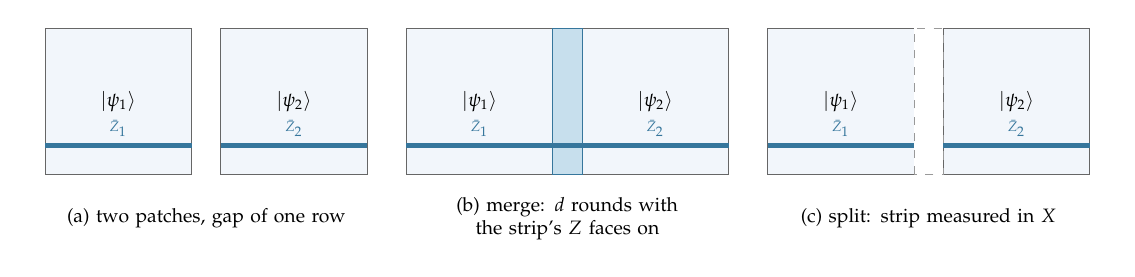
\begin{tikzpicture}[scale=0.62]
% three stages: separate patches, merged, split
\foreach \k/\lab in {0/{(a) two patches, gap of one row},1/{(b) merge: $d$ rounds with the strip's $Z$ faces on},2/{(c) split: strip measured in $X$}}{
  \begin{scope}[xshift=\k*7.4cm]
  \fill[gateblue,draw=black!60] (0,0) rectangle (3,3);
  \fill[gateblue,draw=black!60] (3.6,0) rectangle (6.6,3);
  \node[font=\scriptsize] at (1.5,1.5) {$\ket{\psi_1}$}; \node[font=\scriptsize] at (5.1,1.5) {$\ket{\psi_2}$};
  \draw[cZ!80!black,line width=1.6pt] (0,0.6) -- (3,0.6); \node[font=\tiny,text=cZ!80!black] at (1.5,0.95) {$\bar Z_1$};
  \draw[cZ!80!black,line width=1.6pt] (3.6,0.6) -- (6.6,0.6); \node[font=\tiny,text=cZ!80!black] at (5.1,0.95) {$\bar Z_2$};
  \ifnum\k=1 \fill[cZ!30,draw=cZ!80!black] (3,0) rectangle (3.6,3); \draw[cZ!80!black,line width=1.6pt] (3,0.6) -- (3.6,0.6); \fi
  \ifnum\k=2 \fill[white,draw=black!40,dashed] (3,0) rectangle (3.6,3); \fi
  \node[font=\scriptsize,align=center,text width=4.3cm] at (3.3,-0.9) {\lab};
  \end{scope}}
\end{tikzpicture}
\caption{Measuring $\bar Z_1\bar Z_2$ by lattice surgery. The two patches' $Z$ boundaries face each other across a one-qubit-wide strip prepared in $\ket+$; switching on the strip's $Z$ faces for $d$ rounds measures them, and their product (times already-known boundary checks) is $\bar Z_1\bar Z_2$, read as the parity of the new outcomes; the merged object is a single wider patch encoding one qubit. Measuring the strip in $X$ splits it again, leaving $\ket{\psi_1\psi_2}$ projected onto the $\bar Z_1\bar Z_2=\pm1$ eigenspace, up to a known Pauli frame update. $\bar X_1\bar X_2$ is the same with the $X$ boundaries.}
\label{fig:surgery}
\end{figure}

\begin{itemize}[leftmargin=*]
\item \textbf{$M_{ZZ}$, $M_{XX}$} (\cref{fig:surgery}): $d$ rounds each, because the new checks must themselves be measured $d$ times to be trusted. The outcome has a logical error of order $p_L(d)$ and the patches keep their distance throughout.
\item \textbf{CNOT} $=$ an ancilla patch $\ket{+_L}$, $M_{ZZ}$ between control and ancilla, $M_{XX}$ between ancilla and target, then $M_Z$ of the ancilla, with Pauli corrections from the three outcomes: $2d$ rounds plus the single-qubit measurement, three patches of space. Equivalently, teleport through the ancilla \cite{horsman12,fowler-gidney18}.
\item \textbf{Hadamard}: transversal $H$ on a patch swaps its $X$ and $Z$ boundaries; to restore the standard orientation the patch is \emph{rotated} by growing it into an adjacent ancilla region and shrinking back ($\approx3d$ rounds), or the orientation is simply remembered.
\item \textbf{$S$ and $S^\dagger$}: a $\bar Y$ measurement, which lattice surgery provides through a \emph{twist defect} on the patch boundary, or $M_{ZZ}$ with an ancilla in $\ket{Y_L}$ (a stabiliser state, preparable once and reused: $S=M_{ZZ}$ with $\ket Y$ followed by a Pauli correction) \cite{litinski19game}.
\item \textbf{Multi-qubit Pauli product measurements}: an ancilla region touching several patches measures $\bar P_1\otimes\cdots\otimes\bar P_k$ in one shot of $d$ rounds; Litinski's layouts arrange patches in rows with one row of ancilla space so that any product is reachable \cite{litinski19game}.
\end{itemize}

\paragraph{Pauli and Clifford frames.}\label{sec:frames} No Pauli correction is ever applied to the qubits: the decoder's output is a classical \emph{Pauli frame} that is updated and consulted when a measurement outcome is interpreted, because Paulis commute or anticommute with everything else in a known way \cite{knill05}. Litinski's \emph{game of surface codes} \cite{litinski19game} extends this to Cliffords: any Clifford$+T$ circuit is rewritten as a sequence of $\pi/8$ Pauli-product rotations $e^{-i\frac\pi8P_j}$ (one per $T$ gate, with $P_j$ a multi-qubit Pauli) followed by a final layer of Pauli measurements, by commuting every Clifford to the end of the circuit and absorbing it into the measurement basis. Each $\pi/8$ rotation is then one Pauli product measurement $P_j\otimes\bar Z$ against a magic state (\cref{sec:magic}), a Clifford correction $e^{\pm i\frac\pi4P_j}$ that is itself pushed to the end, and the final Pauli measurements are read in whatever basis the accumulated Clifford dictates. Logical Clifford gates thus cost \emph{nothing} in physical time; the entire runtime is the sequence of Pauli product measurements, one \emph{tick} of $d$ cycles each in the ``fast'' layout---the ``reaction-limited'' regime of \cref{sec:physical}, where the time per $T$ is the classical reaction time (decode, update the frame, choose the next measurement basis) and not the gate time. IonQ's \emph{Clifford frame} is the same idea applied to a trapped-ion LDPC machine: only Pauli measurements and non-Clifford state injections are physically executed, and the Cliffords---including the transversal ones the codes do have---are classical bookkeeping \cite{walkingcat26,haener26}. This is also why Part~I's cost model counts Toffolis and nothing else: Cliffords are free at the logical level, and a Toffoli is four non-Clifford rotations.

\paragraph{Clifford gates on LDPC codes.} With no boundaries to merge, bicycle codes get their Cliffords from automorphisms (qubit permutations that preserve the code, each a logical Clifford on all $12$ qubits at once) and from the generalised surgery of their LPU (\cref{sec:bb}), where a logical Pauli product is measured by attaching an ancilla system for $\approx d$ rounds; IBM's instruction set contains $12$ automorphisms ($14$ timesteps), $15$ in-module and $36$ inter-module Pauli measurements ($120$ timesteps for the gross code), and the frame does the rest \cite{yoder25tour,cross24surgery}. Colour-code machines (Quantinuum, Google's 2024 experiment) use transversal $H$, $S$ and CNOT directly and lattice surgery between colour-code patches for the rest \cite{ryan-anderson24,lacroix24color}; neutral-atom arrays move whole blocks on top of one another for transversal CNOTs between any two blocks \cite{bluvstein24}.

\section{Fault-tolerant $T$ gates}\label{sec:ft-t}

\subsection{Why $T$ is the expensive gate}
Clifford circuits are classically simulable (Gottesman--Knill), so a universal machine needs one gate outside the Clifford group; $T=\mathrm{diag}(1,e^{i\pi/4})$ is the standard choice because it is the cheapest member of the third level of the Clifford hierarchy and because Toffoli $=$ CCZ $+$ Hadamards $=$ seven $T$ gates in the textbook decomposition, four with measurement-based uncomputation (\cref{sec:mbu}). By Eastin--Knill and Bravyi--K\"onig no 2D code has a transversal $T$, so the $T$ gate is \emph{teleported in} from a resource state:
\begin{equation}\label{eq:magic}
\ket T=T\ket+=\tfrac1{\sqrt2}\big(\ket0+e^{i\pi/4}\ket1\big),
\end{equation}
by the gadget of \cref{fig:tgadget}: a CNOT from the data to the magic state and a $Z$ measurement of the magic state apply $T$ to the data up to a Clifford $S$ correction that depends on the outcome---and that correction goes into the Clifford frame. In lattice-surgery form the gadget is one $M_{ZZ}$ between the data patch and the magic-state patch followed by $M_X$ of the magic patch, i.e.\ one tick. So the cost of a $T$ gate is the cost of one $\ket T$ of sufficient quality, and the whole subject reduces to producing $\ket T$ states with error far below $1/(\text{number of }T\text{ gates})$: for the \ecdsafail{} circuits, $4\times28\times1.5\times10^6\approx1.7\times10^8$ $T$ gates per run, i.e.\ a per-state error of order $10^{-10}$.

\begin{figure}[H]
\centering
\begin{quantikz}[column sep=8pt,row sep=5pt,font=\small]
\lstick{$\ket\psi$} & \ctrl{1} & \qw & \gate{S^{m}} & \qw\rstick{$T\ket\psi$} \\
\lstick{$\ket T$} & \targ{} & \meter{m} \setwiretype{c} & \ctrl{-1} &
\end{quantikz}
\hspace{12mm}
\begin{quantikz}[column sep=8pt,row sep=5pt,font=\small]
\lstick{$\ket\psi$} & \gate[2]{M_{ZZ}} & \qw & \gate{S^{m\oplus m'}}\qw & \qw\rstick{$T\ket\psi$ (frame)} \\
\lstick{$\ket{T_L}$} & & \meter{M_X} &
\end{quantikz}
\caption{$T$-gate teleportation. Left: with outcome $m=0$ the data is $T\ket\psi$; with $m=1$ it is $\omega\,T^\dagger\ket\psi$ and $S\,T^\dagger=T$ fixes it ($\omega=e^{i\pi/4}$). Right: the lattice-surgery version, a joint $Z\otimes Z$ measurement (outcome $m$) and an $X$ measurement of the magic patch (outcome $m'$); the $S$ correction is never applied, only recorded.}
\label{fig:tgadget}
\end{figure}

\subsection{Magic-state injection and distillation}\label{sec:magic}\label{sec:distillation}
\paragraph{Injection.} A physical $\ket T$ is prepared by a single-qubit rotation on one data qubit of a $d=1$ patch, which is then grown to distance $d$ by switching on checks around it; during the first rounds the state is unprotected, so the injected logical state has an error of order $p$ (a few $10^{-3}$ for $p=10^{-3}$, $\approx1\%$ in Google's colour-code experiment before post-selection) \cite{lacroix24color}. Injected states are therefore \emph{distilled}.

\paragraph{15-to-1 distillation.} Bravyi and Kitaev's protocol \cite{bravyi-kitaev05} uses the $\bits{15}{1}{3}$ code's transversal $T$ (\cref{sec:smallcodes}). First note that any noisy $\ket T$ can be \emph{twirled} (randomly conjugated by the Clifford $SX$, which fixes $\ket T$) into the form $(1-\epsilon)\ket T\!\bra T+\epsilon\,Z\ket T\!\bra T Z$: a magic state with error is a magic state with a $Z$ error of probability $\epsilon$. Then:
\begin{algorithm}[H]
\caption{15-to-1 magic-state distillation}\label{alg:15to1}
\begin{algorithmic}[1]
\State prepare $\ket{+_L}$ of the $\bits{15}{1}{3}$ Reed--Muller code (a stabiliser state: $\ket+^{\otimes15}$ projected by the ten $Z$-checks, \cref{sec:encoding})
\State apply $T$ transversally by teleporting $15$ noisy $\ket T$ states, one into each qubit, with the gadget of \cref{fig:tgadget} ($15$ $S$ corrections tracked)---the block is now $\bar T^\dagger\ket{+_L}=\ket{T^\dagger_L}$ up to $Z$ errors at the positions of the faulty input states
\State measure the four $X$-type stabilisers; \textbf{if} any is $-1$ \textbf{reject} (a $Z$ error of weight $\le2$ has been detected)
\State decode: measure the fourteen non-data qubits so as to map $\ket{T^\dagger_L}$ to a single qubit (the inverse of the encoder of \cref{alg:encoder}, or a direct $Z$-basis readout of the code with the logical value extracted), apply $S^\dagger$ to turn $\ket{T^\dagger}$ into $\ket T$
\end{algorithmic}
\end{algorithm}
A $Z$ error passes undetected only if it is a $Z$-logical of the code, and the lightest $Z$-logicals have weight three: there are $35$ of them (the lines of the projective space $PG(3,2)$), so the output error is $35\epsilon^3+O(\epsilon^4)$ with acceptance probability $1-15\epsilon+O(\epsilon^2)$. From $\epsilon=10^{-3}$ one round gives $3.5\times10^{-8}$ and two rounds $1.5\times10^{-21}$; in practice the \emph{implementation} of the protocol in the surface code is itself noisy, and that is what sets the floor. Bravyi and Haah's $(3k+8)$-to-$k$ protocols \cite{bravyi-haah12} distil $k$ states at once with output error $(3k+1)\epsilon^2$---quadratic, not cubic, but with far better yield---and are used as second stages. Litinski's surface-code \emph{factories} \cite{litinski19magic} spell out the cost: at $p=10^{-3}$ a single-level $(15\text{-to-}1)_{17,7,7}$ factory occupies $4{,}620$ physical qubits and produces one $\ket T$ of error $4.5\times10^{-8}$ every $42.6$ cycles; a two-level $(15\text{-to-}1)^6_{13,5,5}\times(20\text{-to-}4)_{23,11,13}$ factory, $43{,}300$ qubits, one state of error $1.4\times10^{-10}$ every $130$ cycles; and $(15\text{-to-}1)^6_{13,7,7}\times(8\text{-to-CCZ})_{25,15,15}$, $47{,}000$ qubits, one $\ket{CCZ}$ of error $5.2\times10^{-11}$ every $60$ cycles, where the subscripts are the code distances of the two levels. Gidney and Fowler's CCZ factory with the catalysed $\ket{CCZ}\to2\ket T$ conversion \cite{gidney-fowler19ccz} is the design behind the ``one CCZ per $150$ cycles per factory'' of Model S in \cref{sec:physical}: a Toffoli is then \emph{one} magic state, not four.

\paragraph{Cultivation.} Gidney, Shutty and Jones \cite{cultivation24} replaced the first distillation level by \emph{magic state cultivation}: prepare $\ket T$ in a small colour code ($d=3$, then $5$) where $T$ is transversal, repeatedly \emph{check} the state by measuring the transversal $\bar T$-conjugated stabilisers and post-select, then ``escape'' into a surface code of distance $15$ by growing the patch. The whole thing fits in one patch, costs about as many physical gates as a lattice-surgery CNOT of the same reliability, and gives $\ket T$ states at $2\times10^{-9}$ for $p=10^{-3}$ ($4\times10^{-11}$ at $p=5\times10^{-4}$)---an order of magnitude fewer qubit-rounds than distillation to the same error, and enough that the authors suggest distillation may no longer be needed in practice. Google's RSA-2048 and ECDLP-256 estimates both use it ($\approx5\times10^4$ qubit-rounds per $T$, $\approx25{,}000$ qubits devoted to magic states) \cite{gidney25rsa,babbush26}; the neutral-atom estimate cultivates in surface-code patches of $\approx500$ qubits and then distils $8T\to CCZ$ inside bicycle-code factories to reach $\le10^{-10}$ per CCZ \cite{cain26}; IonQ's two-level CCZ factory produces states below $10^{-9}$ in $319$ qubits each, four of them making a CCZ in under $28$\,ms \cite{haener26}.

\paragraph{Experiments.} Logical magic-state preparation and distillation have been demonstrated: QuEra/Harvard distilled logical magic states in $\bits{5}{1}{3}$ and $\bits{7}{1}{3}$ codes on a neutral-atom array in 2024 \cite{rodriguez24distill}; Google injected magic states into a colour code at $>99\%$ fidelity with post-selection \cite{lacroix24color}.

\subsection{Code switching and gauge fixing}\label{sec:codeswitch}
The alternative to magic states is to carry the logical qubit into a code where $T$ \emph{is} transversal and back. Anderson, Duclos-Cianci and Poulin \cite{anderson14} gave the fault-tolerant conversion between the Steane code (transversal Cliffords) and the $\bits{15}{1}{3}$ Reed--Muller code (transversal $T$): the two are gauge fixings of one $\bits{15}{7}{3}$ subsystem code, and one converts by measuring the stabilisers that the target code has and the source does not (the weight-four $Z$-checks of \cref{sec:smallcodes} when going to Reed--Muller, weight-four $X$-type operators when coming back), correcting with Paulis chosen from the outcomes, and repeating the measurements to make them fault tolerant \cite{paetznick-reichardt13}. Bomb\'in's gauge colour codes do the same in a topological setting (\cref{sec:colour}): the 3D code's face operators are gauge degrees of freedom, fixing them as $Z$-type stabilisers gives transversal $T$, fixing them as $X$-type gives transversal Cliffords, and the switch is a measurement of the operators being fixed \cite{bombin15}. Code switching avoids factories but needs 3D codes ($n\sim d^3$) or small concatenated codes with low thresholds, which is why no large-scale estimate to date uses it; its cost per $T$ is a full syndrome-extraction cycle of the larger code rather than a magic state.

\subsection{What a Toffoli costs, by architecture}
\begin{table}[H]
\centering\footnotesize
\setlength{\tabcolsep}{4pt}
\begin{tabular}{@{}p{3.6cm}p{3.5cm}p{3.6cm}p{4.8cm}@{}}
\toprule
architecture & non-Clifford resource & per-Toffoli time & qubits for magic states\\
\midrule
surface code, superconducting, Model S (\cref{sec:physical}) & $\ket{CCZ}$ from distillation factories \cite{gidney-fowler19ccz} & $150$ cycles per factory; $6$ factories $\Rightarrow25\,\mu$s & six factories inside the $7\times18$-patch compute block ($170{,}352$ physical qubits with workspace)\\
surface code, Google 2025--26 \cite{gidney25rsa,babbush26} & cultivation \cite{cultivation24}, $\approx5\times10^4$ qubit-rounds per $T$ & reaction-limited: $\approx10\,\mu$s reaction $\times$ $1.5$ per Toffoli & $\approx25{,}000$\\
bicycle architecture, IBM \cite{yoder25tour} & factory in a bicycle module & $T$ injection $=$ one inter-module measurement, $120$ timesteps & $454$ per module at $p=10^{-3}$ ($810$ at $10^{-4}$)\\
walking cat, IonQ \cite{walkingcat26,haener26} & two-level CCZ factory in an LDPC code, $<10^{-9}$ & $29.5$\,ms (one measurement layer) & $4\times319=1{,}276$\\
neutral atoms, Cain et al.\ \cite{cain26} & cultivation $+$ $8T\to CCZ$ in $\bits{248}{10}{18}$ factories, $\le10^{-10}$ & $\ge4d$ stabiliser cycles of $1$\,ms & $\approx500$ per cultivation site plus factory codes\\
cat qubits, Alice\,\&\,Bob \cite{gouzien23} & off-line Toffoli-state preparation by projective measurements & $500$\,ns cycle; $9$\,h total & included in $126{,}133$\\
\bottomrule
\end{tabular}
\caption{The non-Clifford gate across the architectures compared in \cref{sec:physical}.}
\label{tab:toffoli-arch}
\end{table}

\section{Physical-qubit estimates}\label{sec:physical}

\subsection{From a logical circuit to a machine}
A logical circuit is characterised by three numbers: its logical qubits $Q$, its non-Clifford gate count $T$ (Toffolis here), and its non-Clifford \emph{depth}. A fault-tolerant machine is characterised by its code, its physical error rate $p$, its cycle time $t_c$ and its reaction time $t_r$ (the classical latency from a measurement to the next basis choice). The estimate proceeds in four steps, which every published number in \cref{tab:external-phys} follows in some form \cite{fowler-gidney18,litinski19game,gidney-ekera21,gidney25rsa}:
\begin{enumerate}[leftmargin=*]
\item \textbf{Error budget.} The run must succeed with reasonable probability, so the total logical error must be $O(1)$: with $Q'$ logical qubits (circuit plus workspace) alive for $R$ rounds, $Q'R\,p_L(d)\lesssim1$, where $R=t_{\rm run}/t_c$. For $Q'\approx1{,}300$ and a run of $10^9$ rounds this is $p_L\lesssim10^{-12}$; Model S below uses $10^{-15}$ per patch per round, i.e.\ $p_{\rm ok}\approx0.999$ for the fast circuits.
\item \textbf{Distance.} From \cref{eq:plaw}, the smallest odd $d$ with $A(p/p_{\rm th})^{(d+1)/2}\le\varepsilon$; the footprint of a logical qubit is $2d^2-1$ physical qubits plus routing space, $2(d+1)^2$ in the layouts of \cite{gidney-ekera21,gidney25rsa}.
\item \textbf{Magic-state supply.} Enough factories (or cultivation sites) to deliver $T$ states at the rate the circuit consumes them; their footprint is added to $Q'$.
\item \textbf{Time.} The larger of the \emph{throughput} bound (gates $\times$ time per magic state) and the \emph{reaction} bound (non-Clifford depth $\times$ $t_r$, because each layer of $T$ gates must be decoded before the next basis is chosen, \cref{sec:frames}); then divide by the success probability and multiply by the expected number of shots.
\end{enumerate}

\subsection{Model S: a surface-code machine at $p=10^{-3}$}\label{sec:modelS}
Model S is the superconducting surface-code model of \code{shor/shor\_qiskit/physical.py}, re-implemented in \code{scripts/physical\_estimates.py} so that the two agree to the qubit: $p=10^{-3}$, $t_c=1\,\mu$s, $t_r=10\,\mu$s, $A=0.1$ and $p_{\rm th}=1.22\%$ (the crossing of \cref{fig:threshold}), target $10^{-15}$ per patch per round $\Rightarrow d=25$, $1{,}352$ physical qubits per logical qubit, a compute block of $7\times18$ patches ($170{,}352$ physical qubits: six CCZ factories of the Gidney--Fowler type and three columns of workspace) delivering one $\ket{CCZ}$ every $25\,\mu$s, so that
\begin{equation}\label{eq:modelS}
\begin{aligned}
N_{\rm phys}&=1{,}352\,Q+170{,}352, & t_{\rm run}&=\max\big(25\,\mu\mathrm{s}\times T,\ 10\,\mu\mathrm{s}\times\text{depth}\big),\\
p_{\rm ok}&=(1-10^{-15})^{(Q+126)\,t_{\rm run}/t_c}.
\end{aligned}
\end{equation}
The ripple-carry circuits of Part~I have a Toffoli depth of $0.8$--$0.95\times T$, so they are throughput-bound in this model (the reaction bound would need depth $<0.4\,T$), and the time is simply $25\,\mu$s per Toffoli. For the \ecdsafail{} rows the challenge's point-addition numbers are converted to a whole attack by \cref{eq:full-attack}: $28$ additions, each with its $3\cdot2^{16}$ lookup Toffolis, and $16$ window qubits added to $Q$.

\begin{table}[H]
\centering\scriptsize
\setlength{\tabcolsep}{3.5pt}
\begin{tabular}{@{}p{6.9cm}rrrrrr@{}}\toprule
circuit (whole attack unless noted) & $Q$ & Toffolis & physical & time/run & $p_{\rm ok}$ & expected\\
\midrule
\ecdsafail{} \code{8e9c9a2} (26 Jul, $1{,}151\times1.30$\,M) $+16$ window qubits & 1,167 & $41.9$\,M & 1,748,136 & 17\,min & 0.999 & 17\,min\\
\ecdsafail{} windowed \code{8e9c9a2} (Note F, lookups included) & 1,162 & $47.1$\,M & 1,741,376 & 20\,min & 0.998 & 20\,min\\
\ecdsafail{} \code{a02c716} (7 Oct, Leapfrog, $1{,}244\times0.80$\,M) $+16$ & 1,260 & $27.8$\,M & 1,873,872 & 12\,min & 0.999 & 12\,min\\
\ecdsafail{} \code{b6f2b0a} low-$Q$ ($825\times489$\,M) $+16$ & 841 & $13.70$\,B & 1,307,384 & 4.0\,d & 0.718 & 5.5\,d\\
\ecdsafail{} \code{10177cd} low-$Q$ ($792\times657$\,M, 7 Oct) $+16$ & 808 & $18.39$\,B & 1,262,768 & 5.3\,d & 0.651 & 8.2\,d\\
Google, Babbush et al.\ low-qubit variant \cite{babbush26} & 1,200 & $90.0$\,M & 1,792,752 & 38\,min & 0.997 & 38\,min\\
Google, Babbush et al.\ low-gate variant \cite{babbush26} & 1,450 & $70.0$\,M & 2,130,752 & 29\,min & 0.997 & 29\,min\\
IonQ, H\"aner et al.\ \cite{haener26} & 1,457 & $39.0$\,M & 2,140,216 & 16\,min & 0.998 & 16\,min\\
Schrottenloher, space-optimised \cite{schrottenloher26} & 1,208 & $72.5$\,M & 1,803,568 & 30\,min & 0.998 & 30\,min\\
Schrottenloher, gate-optimised \cite{schrottenloher26} & 1,462 & $57.7$\,M & 2,146,976 & 24\,min & 0.998 & 24\,min\\
\code{shor/}: IonQ cells, signed windows, SELECT-SWAP (executed) & 1,457 & $36.8$\,M & 2,140,216 & 15\,min & 0.999 & 15\,min\\
\code{shor/}: dialog GCD on the space cells & 1,246 & $79.1$\,M & 1,854,944 & 33\,min & 0.997 & 33\,min\\
\code{shor/}: three field registers, Luo EEA & 851 & $2.39$\,B & 1,320,904 & 16.6\,h & 0.943 & 17.6\,h\\
RSA-2048, Gidney 2025 inputs (for calibration) \cite{gidney25rsa} & 1,399 & $6.50$\,B & 2,061,800 & 45.1\,h & 0.781 & 2.4\,d\\
\bottomrule\end{tabular}

\caption{Model S applied to the \ecdsafail{} circuits, to the published logical costs, and to the \code{shor/} circuits (computed, \code{scripts/physical\_estimates.py}; the logical inputs of each row are cited in \cref{tab:external} and \cref{sec:shor-impl}). ``expected'' divides the run time by $p_{\rm ok}$ (and multiplies by the expected number of shots where a source specifies more than one). The RSA-2048 row feeds Gidney's logical inputs through the same model; his published figure---under a million qubits, under a week---uses yoked storage for idle qubits and cultivation, which this model does not, so the row shows the model's conservatism rather than a discrepancy.}
\label{tab:modelS}
\end{table}

Three things stand out. First, the \emph{physical} cost of every fast 256-bit ECDLP circuit in this model is $1.7$--$2.1$ million qubits and $12$--$40$ minutes: the $Q$ axis of the challenge moves the qubit count by at most $20\%$ because $Q$ is multiplied by one patch footprint, and the $T$ axis moves the time linearly. Second, the low-$Q$ track buys a $25\%$ smaller machine ($1.26$--$1.31$ million qubits) at the price of five to eight days and a success probability of $0.65$--$0.72$ per run, which is why no architecture paper optimises for $Q$ alone: in spacetime volume (qubits $\times$ seconds) the low-$Q$ circuits are $400\times$ more expensive. Third, the \ecdsafail{} frontier's $\QT$ is a reasonable proxy for this volume---$N_{\rm phys}\,t_{\rm run}\approx(1{,}352Q+170{,}352)\times25\,\mu\mathrm{s}\times28(T+3\cdot2^{16})$---but with a $170$k-qubit constant and a $3\cdot2^{16}$-Toffoli constant that the challenge metric omits, both of which favour the fast circuits more than the metric does.

\subsection{Per-gate accounting}
For the reader who wants to rebuild the table from the gate level, at $d=25$ and $p=10^{-3}$:
\begin{itemize}[leftmargin=*]
\item a \textbf{logical qubit} is a $25\times25$ data array with $624$ measure qubits, $1{,}249$ physical qubits, $1{,}352$ with its share of routing; it costs one cycle of $1\,\mu$s per round to keep alive at $\approx10^{-15}$ error;
\item a \textbf{lattice-surgery CNOT} or Pauli product measurement occupies an ancilla region of the same width for $d=25$ rounds, $25\,\mu$s; a Hadamard with patch rotation about $3d$ rounds; Paulis and the Clifford frame are free;
\item a \textbf{$T$ gate} consumes one magic state and one tick of $d$ rounds; a Litinski $(15\text{-to-}1)_{17,7,7}$ factory ($4{,}620$ qubits) delivers one state of error $4.5\times10^{-8}$ every $42.6$ cycles, the two-level factories of \cref{sec:distillation} deliver $10^{-10}$--$10^{-11}$ states in $43$--$47$k qubits every $60$--$130$ cycles, and cultivation delivers $2\times10^{-9}$ states for $\approx5\times10^4$ qubit-rounds each \cite{litinski19magic,cultivation24};
\item a \textbf{Toffoli} is one $\ket{CCZ}$ (Model S: one every $25\,\mu$s from six factories) or four $T$ states plus the measurement-based uncomputation of \cref{sec:mbu}; the \ecdsafail{} 26-July circuit's $4.2\times10^7$ Toffolis are $1.7\times10^8$ $T$ gates, so the magic states must be below $\approx10^{-9}$ each---which the two-level factories and cultivation provide, and the single-level factory does not.
\end{itemize}

\subsection{The published estimates}
\begin{table}[H]
\centering\scriptsize
\setlength{\tabcolsep}{3pt}
\begin{tabular}{@{}p{2.8cm}p{2.4cm}p{2.4cm}p{2.1cm}p{2.0cm}p{3.5cm}@{}}
\toprule
source & platform, code & logical cost & physical qubits & time & assumptions\\
\midrule
Google, Babbush et al.\ 2026 \cite{babbush26} & superconducting, surface code with yoked storage, cultivation & $<1{,}200$ Q, $<90$\,M Toffoli; or $<1{,}450$ Q, $<70$\,M & $<500{,}000$ & $\approx23$ / $18$\,min & $p=10^{-3}$, $1\,\mu$s cycle, $10\,\mu$s reaction $+50\%$ per Toffoli; $\approx25{,}000$ qubits for magic states; circuits withheld\\
IonQ, H\"aner et al.\ 2026 \cite{haener26,walkingcat26} & trapped ions, $\bits{102}{22}{9}$ walking cat & $1{,}457$ Q, $39$\,M Toffoli & $19{,}397$ & $25.7$ days ($63\%$ success) & $p_{2q}=10^{-4}$, $p_{1q}=10^{-5}$, $29.5$\,ms per Toffoli layer; four $319$-qubit CCZ factories\\
PsiQuantum, Litinski 2023 \cite{litinski23,litinski22active} & photonic, active-volume architecture & $\approx50$\,M Toffoli (title) & $6{,}000$ modules $\times1{,}152$ & one key per $10$\,min & non-local module connections; $38$\,h per key for a strictly 2D-local layout\\
Alice\,\&\,Bob, Gouzien et al.\ 2023 \cite{gouzien23} & cat qubits, repetition code & (256-bit ECDLP, Shor) & $126{,}133$ cat qubits & $9$\,h & $\kappa_1/\kappa_2=10^{-5}$, $19$ photons, $500$\,ns cycle, lattice surgery, off-line Toffoli states\\
Neutral atoms, Cain et al.\ 2026 \cite{cain26} & reconfigurable atoms, lifted-product $\bits{2610}{744}{\le16}$ memory, $\bits{248}{10}{\le18}$ processor & (P-256, Shor) & $\approx26{,}000$ (balanced $11{,}961$; space-efficient $9{,}739$) & ``a few days'' (fastest $\approx10$ days at $10$--$26$k) & $p=10^{-3}$ ($0.093\%$ for the fastest), $1$\,ms stabiliser cycle, cultivation $+$ $8T\!\to\!CCZ$; RSA-2048 $\approx100\times$ longer\\
Kim et al.\ 2026 \cite{kim26} & surface code; or QLDPC (Pinnacle model) & P-256: $7{,}454$ Q, $1.39$\,B Toffoli (in-place) & $11.7$\,M (surface) / $765{,}234$ (QLDPC) & $23.9$\,min / $21.9$\,h & $p=10^{-3}$, $1\,\mu$s, $10\,\mu$s reaction; 15-to-1 distillation\\
Iceberg, Pinnacle 2026 \cite{pinnacle26} & QLDPC & RSA-2048 & $<100{,}000$ & -- & $p=10^{-3}$, $1\,\mu$s, $10\,\mu$s reaction\\
Google, Gidney 2025 \cite{gidney25rsa} & surface code, yoked storage, cultivation & RSA-2048: $\approx6.5$\,B Toffoli & $<1$\,M & $<1$ week & $p=10^{-3}$, $1\,\mu$s, $10\,\mu$s reaction\\
Model S, this document & surface code, factories & 26-Jul \ecdsafail{} $+$ windows & $1.75$\,M & $17$\,min & \cref{eq:modelS}\\
\bottomrule
\end{tabular}
\caption{Published physical estimates for 256-bit ECDLP (and the RSA-2048 points that use the same machinery), from the companies' and authors' arXiv/ePrint papers (\cref{app:sources}). ``Q'' is logical qubits. The platforms differ by two orders of magnitude in clock speed and in physical qubit count in opposite directions, which is why the time-to-key and the qubit count must be read together.}
\label{tab:external-phys}
\end{table}

The ordering in \cref{tab:external-phys} is the ordering of \emph{clock speeds}: superconducting circuits at $1\,\mu$s per cycle run the $4\times10^7$-Toffoli circuit in minutes on $10^5$--$10^6$ qubits; trapped ions at $30$\,ms per Toffoli layer take weeks but need $20{,}000$ ions because high-rate codes and all-to-all connectivity shrink both the code and the factories; neutral atoms sit between, with $1$\,ms cycles and $10$--$26$k atoms; cat qubits use a biased-noise code that needs only a repetition code ($126$k cat qubits, nine hours). Google's half-million figure for the same logical circuit as Model S's two million comes from three choices this document's model does not make---storing idle logical qubits in yoked codes, which packs them two to three times denser, cultivating magic states instead of running factories ($25$k qubits instead of $170$k), and tuning the distance to the actual run length---and from reaction-limited rather than throughput-limited timing ($10\,\mu$s $\times1.5$ per Toffoli $\approx15\,\mu$s instead of $25\,\mu$s) \cite{babbush26}.

\paragraph{An LDPC illustration.} IBM has published no ECDLP estimate, but its per-instruction numbers \cite{yoder25tour} allow an order-of-magnitude placement of the bicycle architecture. A two-gross module ($576$ code $+158$ LPU $+34$ adapter $+463$ factory at $p=10^{-3}$, $\approx1{,}230$ physical qubits) holds $12$ logical qubits with an in-module measurement error of $\approx10^{-11}$ per $216$ timesteps; $1{,}457$ logical qubits are $122$ modules, $\approx150{,}000$ physical qubits, and the $1.7\times10^8$ $T$ gates of the 26-July circuit would accumulate $\approx2\times10^{-3}$ logical error through their measurements. Each $T$ costs one $216$-timestep measurement; with the circuit's Toffoli depth close to its count the serial time is $\approx1.7\times10^8\times216\,\mu\mathrm{s}\approx10$ hours at a $1\,\mu$s timestep. This is \emph{not} IBM's number---it ignores inter-module routing (the $36$ inter-module measurements cost the same $216$ steps but have higher error on the gross code), the factory throughput and the fact that the gross code, not the two-gross, is the near-term target---but it shows the shape of the LDPC trade: an order of magnitude fewer qubits than the surface code at $p=10^{-3}$, and an order of magnitude more time, because logical operations on an LDPC block are serialised through its LPU rather than performed on all patches at once.

\subsection{What the logical optimisations buy, physically}
Translating Part~I's frontier through \cref{eq:modelS}: the $2{,}715\times3.96$\,M baseline of May is $3.9$\,M qubits and $49$\,min; the 26-July incumbent $1.75$\,M and $17$\,min; the 7-October frontier $1.87$\,M and $12$\,min. The six inversion architectures and the arithmetic levers together bought a factor of two in physical qubits and four in time in this model---the time coming almost entirely from the Toffoli count, the qubits from the width---and the remaining distance to Google's half-million is a matter of the \emph{physical} layer (yoked storage, cultivation), not of the logical circuit. On the trapped-ion side the same $39$\,M-Toffoli circuit costs $19{,}397$ ions and $26$ days, so a further halving of the Toffoli count (the frontier's $0.80$\,M per addition against IonQ's $1.39$\,M) would be worth two weeks there and five minutes on a superconducting machine.

\section{Conclusion}\label{sec:conclusion}

\begin{keybox}[title={The whole picture in six statements}]
\begin{enumerate}[leftmargin=*,itemsep=2pt]
\item The cost of breaking secp256k1 is $28$ windowed point additions, and the cost of a point addition is one modular inversion plus a handful of multiplications; \ecdsafail{} spent five months on that inversion and moved its $\QT$ from $1.08\times10^{10}$ to $1.0\times10^9$ by replacing Kaliski's walk with a sequence of ever-cheaper recorded walks (dialog, Jump-2, ping-pong, Skywalk, Leapfrog), by pricing every comparator and fold against a validator-failure budget $\lambda$, and by sharing registers and venting qubits until the peak was set by a single owner (\cref{sec:opts}).
\item The frontier is two-dimensional and its two ends are far apart: $1{,}244\times0.80$\,M at the fast end, $792$ qubits at the narrow end, with the narrow end costing $800\times$ more Toffolis (\cref{sec:pareto}); the \code{shor/} package sits at $1{,}457\times1.31$\,M with exact or measured-error cells and the generic version of most of the frontier's levers (\cref{sec:shor-impl}).
\item Error correction turns each logical qubit into $\sim10^3$ physical ones and each $T$ gate into a magic state, because the Knill--Laflamme conditions can be met by stabiliser codes whose checks are measured repeatedly and decoded classically, but no 2D code can be universal transversally (\cref{sec:qec-why,sec:ft-clifford}).
\item The surface code is the baseline---threshold $\approx1\%$, $\Lambda\approx10$ per two units of distance at $p=10^{-3}$, matching decoders, lattice surgery for Cliffords, factories or cultivation for $T$---and the quantum LDPC codes (IBM's bicycle codes, IonQ's walking-cat codes, lifted-product codes for atoms) trade a tenfold saving in qubits for serialised logical operations and harder decoding (\cref{sec:codes,sec:codes2}).
\item On a superconducting surface-code machine at $p=10^{-3}$ the fast \ecdsafail{} circuits need $1.7$--$1.9$ million physical qubits and $12$--$20$ minutes in this document's model, or under half a million qubits and $\approx20$ minutes with yoked storage and cultivation in Google's; the same circuits need $\approx20{,}000$ ions and $26$ days, $10$--$26{,}000$ atoms and days, or $126{,}000$ cat qubits and nine hours (\cref{sec:physical}).
\item What the logical optimisations buy physically is time on fast machines and weeks on slow ones; what they cannot buy is the factor between two million and half a million qubits, which belongs to the physical layer.
\end{enumerate}
\end{keybox}

\paragraph{For the \code{shor/} project.} The package's natural next steps, in the order of their physical payoff: a Leapfrog backend behind \code{ec\_gcd.mul} (the whole remaining Toffoli gap of the frontier is in the walk); the fused replay cell and the base-5 codec for the Jump-2 backend; and, on the physical side, a yoked-storage and cultivation variant of \code{physical.py} so that its surface-code numbers can be compared with Google's rather than only with Model S, plus an LDPC module model built from IBM's and IonQ's per-instruction tables (\cref{tab:toffoli-arch}) for the platforms where logical-depth, not Toffoli count, sets the clock.


\clearpage
\appendix
\section{Sources and how they were checked}\label{app:sources}

The brief for this document restricted sources to arXiv, the IACR ePrint archive, and the published material of established quantum-computing companies, with the additional instruction to consult IBM Quantum's resources. The policy applied:

\begin{itemize}[leftmargin=*]
\item \textbf{arXiv and ePrint.} Every paper cited with an arXiv or ePrint identifier was located through its arXiv abstract page (\code{arxiv.org/abs/\ldots}) or its ePrint record, and the numbers quoted from it were taken from the abstract or from the paper's own tables (fetched as the arXiv HTML rendering where the abstract was not enough: \cite{babbush26,haener26,yoder25tour,cain26}). Two papers were read from the user's own copies in \code{shor/papers/}: Schrottenloher \cite{schrottenloher26} (ePrint 2026/1128) and Kim et al.\ \cite{kim26} (ePrint 2026/106).
\item \textbf{Company material.} A source counts as a company source when the paper's arXiv record lists the company as the authors' affiliation or the page is served from the company's own domain. The companies whose material is used, and the form it takes:
  \begin{description}[leftmargin=*,style=nextline]
  \item[Google Quantum AI (\code{quantumai.google}).] Willow below-threshold memory \cite{willow25}; colour code on a superconducting processor \cite{lacroix24color}; AlphaQubit (with Google DeepMind) \cite{alphaqubit24}; yoked surface codes \cite{yoked23}; magic state cultivation \cite{cultivation24}; the colour-code circuits and Chromobius \cite{gidney23color}; the RSA-2048 estimate \cite{gidney25rsa}; the ECDLP-256 estimates and mitigations paper \cite{babbush26}; Stim and PyMatching \cite{gidney21stim,higgott23pymatching}.
  \item[IBM Quantum (\code{ibm.com/quantum}).] The bivariate bicycle (gross) code paper \cite{bravyi24gross}; the bicycle architecture (``Tour de gross'') \cite{yoder25tour}; improved QLDPC surgery \cite{cross24surgery}; Relay-BP \cite{mueller25relaybp}; the June 2025 fault-tolerance announcement \cite{ibm-blog25} and the development roadmap \cite{ibm-roadmap}, both read from \code{ibm.com}; and the IBM Quantum Learning course ``Foundations of quantum error correction'' \cite{ibm-learning-qec}, used as the reference for the pedagogical ordering of \cref{sec:qec-why,sec:codes}.
  \item[IonQ (\code{ionq.com}).] The walking-cat architecture \cite{walkingcat26} and the ECDLP-256 trapped-ion estimate \cite{haener26} (both arXiv, IonQ affiliations; the latter is also ePrint 2026/1916).
  \item[Quantinuum / Honeywell (\code{quantinuum.com}).] Real-time fault-tolerant error correction on the $\bits{7}{1}{3}$ code \cite{ryan-anderson21} and fault-tolerant logical teleportation with transversal gates and lattice surgery \cite{ryan-anderson24}.
  \item[PsiQuantum (\code{psiquantum.com}).] The active-volume architecture \cite{litinski22active} and the ``50 million Toffoli gates'' ECDLP estimate \cite{litinski23}.
  \item[QuEra / Harvard (\code{quera.com}).] The logical processor on reconfigurable atom arrays \cite{bluvstein24} and logical magic-state distillation \cite{rodriguez24distill}; the 2026 neutral-atom Shor estimate \cite{cain26} is from the same Harvard/Caltech group with QuEra co-authors.
  \item[Alice\,\&\,Bob (\code{alice-bob.com}).] The repetition-cat ECDLP-256 estimate \cite{gouzien23} and the repetition-cat proposal \cite{guillaud19}.
  \end{description}
  Iceberg Quantum's Pinnacle architecture \cite{pinnacle26} is included in \cref{tab:external-phys} as an arXiv paper, not as an established-company source.
\item \textbf{The \ecdsafail{} material} is on GitHub: the challenge repository, the supplemental materials of the paper's authors, and the per-commit wiki (\cref{sec:challenge}); the paper itself is on arXiv \cite{ecdsafail26}.
\item \textbf{Textbook material} (stabiliser formalism, the small codes, the threshold theorem, the bounds) is cited to the original arXiv/journal papers \cite{gottesman97,crss98,knill-laflamme97,aharonov-benor08,shor95,steane96,laflamme96,bennett96,kitaev03,dennis02} and to Gottesman's textbook draft \cite{gottesman24book}.
\item \textbf{Computed for this document}: the encoders and syndrome tables of \cref{sec:smallcodes}, the surface-code threshold data of \cref{fig:threshold}, the BB-code verification of \cref{tab:bb}, the BP+OSD simulation of \cref{fig:bposd}, the bounds of \cref{fig:bounds}, the Pareto and trajectory data of \cref{sec:pareto}, and the Model S table. Every such number is marked ``computed'' at the point of use and reproducible from \cref{app:scripts}.
\end{itemize}

\section{Scripts and data}\label{app:scripts}

All scripts are Python~3 and were run with Stim~1.16, PyMatching~2.4 and NumPy; the data files they produce are shipped with the \LaTeX{} source in \code{data/}. Run them from the document's root directory.

\begin{table}[H]
\centering\footnotesize
\begin{tabular}{@{}p{4.7cm}p{6.2cm}p{4.1cm}@{}}
\toprule
script & what it does & output\\
\midrule
\code{surface\_threshold.py} & Stim rotated memory-$Z$ circuits, $d=3,5,7,9$, circuit-level depolarising noise, PyMatching MWPM, $\ge1{,}000$ failures or $12$\,M shots per point; per-round conversion & \code{surface\_threshold.dat} (\cref{fig:threshold})\\
\code{standard\_form\_encoder.py} & Gottesman standard form by Gaussian elimination, encoder emission, Stim verification of stabilisers and logicals for $\bits{5}{1}{3}$, Steane, Shor, $\bits{15}{1}{3}$ & printed circuits (\cref{fig:small-encoders})\\
\code{verify\_codes.py} & Stim check of the textbook Shor and Steane encoders and of the $\bits{5}{1}{3}$ circuit; syndrome uniqueness; RM$_{15}$ CSS structure & printed\\
\code{syndrome\_tables.py} & lookup tables of the small codes; splits \code{codes.dat} by family & \code{syn\_*.tex}, \code{codes\_*.dat}\\
\code{bb\_codes.py} & builds $H_X=[A|B]$, $H_Z=[B^{\mathsf T}|A^{\mathsf T}]$ for the five BB codes, checks orthogonality, weights, degrees and $k$ & printed (\cref{tab:bb})\\
\code{bp\_osd\_gross.py} & min-sum BP ($60$ iterations, $\alpha=0.8$) $+$ OSD-0 on the gross code under code-capacity $X$ noise; logical failure test by rank & \code{bb\_bposd.dat} (\cref{fig:bposd})\\
\code{physical\_estimates.py} & Model S (\cref{eq:modelS}) applied to every row of \cref{tab:modelS}; per-gate accounting & \code{physical\_modelS.json}\\
\code{modelS\_table.py} & formats the JSON as the table & \code{modelS\_table.tex}\\
\bottomrule
\end{tabular}
\end{table}

The Pareto, trajectory and census data of \cref{sec:pareto} (\code{incumbents.dat}, \code{promoted\_qt.dat}, \code{rejected\_qt.dat}, \code{frontier\_oct7\_*.dat}) were extracted from the challenge repository's leaderboard files, the supplemental materials' \code{frontier\_reconstruction/} CSVs and the wiki's 7-October TSV snapshot; \code{bounds.dat} tabulates \cref{eq:singleton,eq:hamming,eq:gv} and \code{codes.dat} the $(n,k,d)$ of the codes in \cref{fig:bounds}.

\subsection*{\code{scripts/standard\_form\_encoder.py}}
\lstinputlisting[style=py,basicstyle=\scriptsize\ttfamily]{scripts/standard_form_encoder.py}
\subsection*{\code{scripts/surface\_threshold.py}}
\lstinputlisting[style=py,basicstyle=\scriptsize\ttfamily]{scripts/surface_threshold.py}
\subsection*{\code{scripts/bb\_codes.py}}
\lstinputlisting[style=py,basicstyle=\scriptsize\ttfamily]{scripts/bb_codes.py}
\subsection*{\code{scripts/bp\_osd\_gross.py}}
\lstinputlisting[style=py,basicstyle=\scriptsize\ttfamily]{scripts/bp_osd_gross.py}
\subsection*{\code{scripts/physical\_estimates.py}}
\lstinputlisting[style=py,basicstyle=\scriptsize\ttfamily]{scripts/physical_estimates.py}
\subsection*{\code{scripts/syndrome\_tables.py}}
\lstinputlisting[style=py,basicstyle=\scriptsize\ttfamily]{scripts/syndrome_tables.py}
\subsection*{\code{scripts/verify\_codes.py}}
\lstinputlisting[style=py,basicstyle=\scriptsize\ttfamily]{scripts/verify_codes.py}


\clearpage
\bibliographystyle{plainnat}
\bibliography{refs}
\end{document}
